
% Default to the notebook output style

    


% Inherit from the specified cell style.




    
\documentclass[11pt]{article}

    
    
    \usepackage[T1]{fontenc}
    % Nicer default font (+ math font) than Computer Modern for most use cases
    \usepackage{mathpazo}

    % Basic figure setup, for now with no caption control since it's done
    % automatically by Pandoc (which extracts ![](path) syntax from Markdown).
    \usepackage{graphicx}
    % We will generate all images so they have a width \maxwidth. This means
    % that they will get their normal width if they fit onto the page, but
    % are scaled down if they would overflow the margins.
    \makeatletter
    \def\maxwidth{\ifdim\Gin@nat@width>\linewidth\linewidth
    \else\Gin@nat@width\fi}
    \makeatother
    \let\Oldincludegraphics\includegraphics
    % Set max figure width to be 80% of text width, for now hardcoded.
    \renewcommand{\includegraphics}[1]{\Oldincludegraphics[width=.8\maxwidth]{#1}}
    % Ensure that by default, figures have no caption (until we provide a
    % proper Figure object with a Caption API and a way to capture that
    % in the conversion process - todo).
    \usepackage{caption}
    \DeclareCaptionLabelFormat{nolabel}{}
    \captionsetup{labelformat=nolabel}

    \usepackage{adjustbox} % Used to constrain images to a maximum size 
    \usepackage{xcolor} % Allow colors to be defined
    \usepackage{enumerate} % Needed for markdown enumerations to work
    \usepackage{geometry} % Used to adjust the document margins
    \usepackage{amsmath} % Equations
    \usepackage{amssymb} % Equations
    \usepackage{textcomp} % defines textquotesingle
    % Hack from http://tex.stackexchange.com/a/47451/13684:
    \AtBeginDocument{%
        \def\PYZsq{\textquotesingle}% Upright quotes in Pygmentized code
    }
    \usepackage{upquote} % Upright quotes for verbatim code
    \usepackage{eurosym} % defines \euro
    \usepackage[mathletters]{ucs} % Extended unicode (utf-8) support
    \usepackage[utf8x]{inputenc} % Allow utf-8 characters in the tex document
    \usepackage{fancyvrb} % verbatim replacement that allows latex
    \usepackage{grffile} % extends the file name processing of package graphics 
                         % to support a larger range 
    % The hyperref package gives us a pdf with properly built
    % internal navigation ('pdf bookmarks' for the table of contents,
    % internal cross-reference links, web links for URLs, etc.)
    \usepackage{hyperref}
    \usepackage{longtable} % longtable support required by pandoc >1.10
    \usepackage{booktabs}  % table support for pandoc > 1.12.2
    \usepackage[inline]{enumitem} % IRkernel/repr support (it uses the enumerate* environment)
    \usepackage[normalem]{ulem} % ulem is needed to support strikethroughs (\sout)
                                % normalem makes italics be italics, not underlines
    

    
    
    % Colors for the hyperref package
    \definecolor{urlcolor}{rgb}{0,.145,.698}
    \definecolor{linkcolor}{rgb}{.71,0.21,0.01}
    \definecolor{citecolor}{rgb}{.12,.54,.11}

    % ANSI colors
    \definecolor{ansi-black}{HTML}{3E424D}
    \definecolor{ansi-black-intense}{HTML}{282C36}
    \definecolor{ansi-red}{HTML}{E75C58}
    \definecolor{ansi-red-intense}{HTML}{B22B31}
    \definecolor{ansi-green}{HTML}{00A250}
    \definecolor{ansi-green-intense}{HTML}{007427}
    \definecolor{ansi-yellow}{HTML}{DDB62B}
    \definecolor{ansi-yellow-intense}{HTML}{B27D12}
    \definecolor{ansi-blue}{HTML}{208FFB}
    \definecolor{ansi-blue-intense}{HTML}{0065CA}
    \definecolor{ansi-magenta}{HTML}{D160C4}
    \definecolor{ansi-magenta-intense}{HTML}{A03196}
    \definecolor{ansi-cyan}{HTML}{60C6C8}
    \definecolor{ansi-cyan-intense}{HTML}{258F8F}
    \definecolor{ansi-white}{HTML}{C5C1B4}
    \definecolor{ansi-white-intense}{HTML}{A1A6B2}

    % commands and environments needed by pandoc snippets
    % extracted from the output of `pandoc -s`
    \providecommand{\tightlist}{%
      \setlength{\itemsep}{0pt}\setlength{\parskip}{0pt}}
    \DefineVerbatimEnvironment{Highlighting}{Verbatim}{commandchars=\\\{\}}
    % Add ',fontsize=\small' for more characters per line
    \newenvironment{Shaded}{}{}
    \newcommand{\KeywordTok}[1]{\textcolor[rgb]{0.00,0.44,0.13}{\textbf{{#1}}}}
    \newcommand{\DataTypeTok}[1]{\textcolor[rgb]{0.56,0.13,0.00}{{#1}}}
    \newcommand{\DecValTok}[1]{\textcolor[rgb]{0.25,0.63,0.44}{{#1}}}
    \newcommand{\BaseNTok}[1]{\textcolor[rgb]{0.25,0.63,0.44}{{#1}}}
    \newcommand{\FloatTok}[1]{\textcolor[rgb]{0.25,0.63,0.44}{{#1}}}
    \newcommand{\CharTok}[1]{\textcolor[rgb]{0.25,0.44,0.63}{{#1}}}
    \newcommand{\StringTok}[1]{\textcolor[rgb]{0.25,0.44,0.63}{{#1}}}
    \newcommand{\CommentTok}[1]{\textcolor[rgb]{0.38,0.63,0.69}{\textit{{#1}}}}
    \newcommand{\OtherTok}[1]{\textcolor[rgb]{0.00,0.44,0.13}{{#1}}}
    \newcommand{\AlertTok}[1]{\textcolor[rgb]{1.00,0.00,0.00}{\textbf{{#1}}}}
    \newcommand{\FunctionTok}[1]{\textcolor[rgb]{0.02,0.16,0.49}{{#1}}}
    \newcommand{\RegionMarkerTok}[1]{{#1}}
    \newcommand{\ErrorTok}[1]{\textcolor[rgb]{1.00,0.00,0.00}{\textbf{{#1}}}}
    \newcommand{\NormalTok}[1]{{#1}}
    
    % Additional commands for more recent versions of Pandoc
    \newcommand{\ConstantTok}[1]{\textcolor[rgb]{0.53,0.00,0.00}{{#1}}}
    \newcommand{\SpecialCharTok}[1]{\textcolor[rgb]{0.25,0.44,0.63}{{#1}}}
    \newcommand{\VerbatimStringTok}[1]{\textcolor[rgb]{0.25,0.44,0.63}{{#1}}}
    \newcommand{\SpecialStringTok}[1]{\textcolor[rgb]{0.73,0.40,0.53}{{#1}}}
    \newcommand{\ImportTok}[1]{{#1}}
    \newcommand{\DocumentationTok}[1]{\textcolor[rgb]{0.73,0.13,0.13}{\textit{{#1}}}}
    \newcommand{\AnnotationTok}[1]{\textcolor[rgb]{0.38,0.63,0.69}{\textbf{\textit{{#1}}}}}
    \newcommand{\CommentVarTok}[1]{\textcolor[rgb]{0.38,0.63,0.69}{\textbf{\textit{{#1}}}}}
    \newcommand{\VariableTok}[1]{\textcolor[rgb]{0.10,0.09,0.49}{{#1}}}
    \newcommand{\ControlFlowTok}[1]{\textcolor[rgb]{0.00,0.44,0.13}{\textbf{{#1}}}}
    \newcommand{\OperatorTok}[1]{\textcolor[rgb]{0.40,0.40,0.40}{{#1}}}
    \newcommand{\BuiltInTok}[1]{{#1}}
    \newcommand{\ExtensionTok}[1]{{#1}}
    \newcommand{\PreprocessorTok}[1]{\textcolor[rgb]{0.74,0.48,0.00}{{#1}}}
    \newcommand{\AttributeTok}[1]{\textcolor[rgb]{0.49,0.56,0.16}{{#1}}}
    \newcommand{\InformationTok}[1]{\textcolor[rgb]{0.38,0.63,0.69}{\textbf{\textit{{#1}}}}}
    \newcommand{\WarningTok}[1]{\textcolor[rgb]{0.38,0.63,0.69}{\textbf{\textit{{#1}}}}}
    
    
    % Define a nice break command that doesn't care if a line doesn't already
    % exist.
    \def\br{\hspace*{\fill} \\* }
    % Math Jax compatability definitions
    \def\gt{>}
    \def\lt{<}
    % Document parameters
    \title{dog\_app\_thomas\_Meng}
    
    
    

    % Pygments definitions
    
\makeatletter
\def\PY@reset{\let\PY@it=\relax \let\PY@bf=\relax%
    \let\PY@ul=\relax \let\PY@tc=\relax%
    \let\PY@bc=\relax \let\PY@ff=\relax}
\def\PY@tok#1{\csname PY@tok@#1\endcsname}
\def\PY@toks#1+{\ifx\relax#1\empty\else%
    \PY@tok{#1}\expandafter\PY@toks\fi}
\def\PY@do#1{\PY@bc{\PY@tc{\PY@ul{%
    \PY@it{\PY@bf{\PY@ff{#1}}}}}}}
\def\PY#1#2{\PY@reset\PY@toks#1+\relax+\PY@do{#2}}

\expandafter\def\csname PY@tok@w\endcsname{\def\PY@tc##1{\textcolor[rgb]{0.73,0.73,0.73}{##1}}}
\expandafter\def\csname PY@tok@c\endcsname{\let\PY@it=\textit\def\PY@tc##1{\textcolor[rgb]{0.25,0.50,0.50}{##1}}}
\expandafter\def\csname PY@tok@cp\endcsname{\def\PY@tc##1{\textcolor[rgb]{0.74,0.48,0.00}{##1}}}
\expandafter\def\csname PY@tok@k\endcsname{\let\PY@bf=\textbf\def\PY@tc##1{\textcolor[rgb]{0.00,0.50,0.00}{##1}}}
\expandafter\def\csname PY@tok@kp\endcsname{\def\PY@tc##1{\textcolor[rgb]{0.00,0.50,0.00}{##1}}}
\expandafter\def\csname PY@tok@kt\endcsname{\def\PY@tc##1{\textcolor[rgb]{0.69,0.00,0.25}{##1}}}
\expandafter\def\csname PY@tok@o\endcsname{\def\PY@tc##1{\textcolor[rgb]{0.40,0.40,0.40}{##1}}}
\expandafter\def\csname PY@tok@ow\endcsname{\let\PY@bf=\textbf\def\PY@tc##1{\textcolor[rgb]{0.67,0.13,1.00}{##1}}}
\expandafter\def\csname PY@tok@nb\endcsname{\def\PY@tc##1{\textcolor[rgb]{0.00,0.50,0.00}{##1}}}
\expandafter\def\csname PY@tok@nf\endcsname{\def\PY@tc##1{\textcolor[rgb]{0.00,0.00,1.00}{##1}}}
\expandafter\def\csname PY@tok@nc\endcsname{\let\PY@bf=\textbf\def\PY@tc##1{\textcolor[rgb]{0.00,0.00,1.00}{##1}}}
\expandafter\def\csname PY@tok@nn\endcsname{\let\PY@bf=\textbf\def\PY@tc##1{\textcolor[rgb]{0.00,0.00,1.00}{##1}}}
\expandafter\def\csname PY@tok@ne\endcsname{\let\PY@bf=\textbf\def\PY@tc##1{\textcolor[rgb]{0.82,0.25,0.23}{##1}}}
\expandafter\def\csname PY@tok@nv\endcsname{\def\PY@tc##1{\textcolor[rgb]{0.10,0.09,0.49}{##1}}}
\expandafter\def\csname PY@tok@no\endcsname{\def\PY@tc##1{\textcolor[rgb]{0.53,0.00,0.00}{##1}}}
\expandafter\def\csname PY@tok@nl\endcsname{\def\PY@tc##1{\textcolor[rgb]{0.63,0.63,0.00}{##1}}}
\expandafter\def\csname PY@tok@ni\endcsname{\let\PY@bf=\textbf\def\PY@tc##1{\textcolor[rgb]{0.60,0.60,0.60}{##1}}}
\expandafter\def\csname PY@tok@na\endcsname{\def\PY@tc##1{\textcolor[rgb]{0.49,0.56,0.16}{##1}}}
\expandafter\def\csname PY@tok@nt\endcsname{\let\PY@bf=\textbf\def\PY@tc##1{\textcolor[rgb]{0.00,0.50,0.00}{##1}}}
\expandafter\def\csname PY@tok@nd\endcsname{\def\PY@tc##1{\textcolor[rgb]{0.67,0.13,1.00}{##1}}}
\expandafter\def\csname PY@tok@s\endcsname{\def\PY@tc##1{\textcolor[rgb]{0.73,0.13,0.13}{##1}}}
\expandafter\def\csname PY@tok@sd\endcsname{\let\PY@it=\textit\def\PY@tc##1{\textcolor[rgb]{0.73,0.13,0.13}{##1}}}
\expandafter\def\csname PY@tok@si\endcsname{\let\PY@bf=\textbf\def\PY@tc##1{\textcolor[rgb]{0.73,0.40,0.53}{##1}}}
\expandafter\def\csname PY@tok@se\endcsname{\let\PY@bf=\textbf\def\PY@tc##1{\textcolor[rgb]{0.73,0.40,0.13}{##1}}}
\expandafter\def\csname PY@tok@sr\endcsname{\def\PY@tc##1{\textcolor[rgb]{0.73,0.40,0.53}{##1}}}
\expandafter\def\csname PY@tok@ss\endcsname{\def\PY@tc##1{\textcolor[rgb]{0.10,0.09,0.49}{##1}}}
\expandafter\def\csname PY@tok@sx\endcsname{\def\PY@tc##1{\textcolor[rgb]{0.00,0.50,0.00}{##1}}}
\expandafter\def\csname PY@tok@m\endcsname{\def\PY@tc##1{\textcolor[rgb]{0.40,0.40,0.40}{##1}}}
\expandafter\def\csname PY@tok@gh\endcsname{\let\PY@bf=\textbf\def\PY@tc##1{\textcolor[rgb]{0.00,0.00,0.50}{##1}}}
\expandafter\def\csname PY@tok@gu\endcsname{\let\PY@bf=\textbf\def\PY@tc##1{\textcolor[rgb]{0.50,0.00,0.50}{##1}}}
\expandafter\def\csname PY@tok@gd\endcsname{\def\PY@tc##1{\textcolor[rgb]{0.63,0.00,0.00}{##1}}}
\expandafter\def\csname PY@tok@gi\endcsname{\def\PY@tc##1{\textcolor[rgb]{0.00,0.63,0.00}{##1}}}
\expandafter\def\csname PY@tok@gr\endcsname{\def\PY@tc##1{\textcolor[rgb]{1.00,0.00,0.00}{##1}}}
\expandafter\def\csname PY@tok@ge\endcsname{\let\PY@it=\textit}
\expandafter\def\csname PY@tok@gs\endcsname{\let\PY@bf=\textbf}
\expandafter\def\csname PY@tok@gp\endcsname{\let\PY@bf=\textbf\def\PY@tc##1{\textcolor[rgb]{0.00,0.00,0.50}{##1}}}
\expandafter\def\csname PY@tok@go\endcsname{\def\PY@tc##1{\textcolor[rgb]{0.53,0.53,0.53}{##1}}}
\expandafter\def\csname PY@tok@gt\endcsname{\def\PY@tc##1{\textcolor[rgb]{0.00,0.27,0.87}{##1}}}
\expandafter\def\csname PY@tok@err\endcsname{\def\PY@bc##1{\setlength{\fboxsep}{0pt}\fcolorbox[rgb]{1.00,0.00,0.00}{1,1,1}{\strut ##1}}}
\expandafter\def\csname PY@tok@kc\endcsname{\let\PY@bf=\textbf\def\PY@tc##1{\textcolor[rgb]{0.00,0.50,0.00}{##1}}}
\expandafter\def\csname PY@tok@kd\endcsname{\let\PY@bf=\textbf\def\PY@tc##1{\textcolor[rgb]{0.00,0.50,0.00}{##1}}}
\expandafter\def\csname PY@tok@kn\endcsname{\let\PY@bf=\textbf\def\PY@tc##1{\textcolor[rgb]{0.00,0.50,0.00}{##1}}}
\expandafter\def\csname PY@tok@kr\endcsname{\let\PY@bf=\textbf\def\PY@tc##1{\textcolor[rgb]{0.00,0.50,0.00}{##1}}}
\expandafter\def\csname PY@tok@bp\endcsname{\def\PY@tc##1{\textcolor[rgb]{0.00,0.50,0.00}{##1}}}
\expandafter\def\csname PY@tok@fm\endcsname{\def\PY@tc##1{\textcolor[rgb]{0.00,0.00,1.00}{##1}}}
\expandafter\def\csname PY@tok@vc\endcsname{\def\PY@tc##1{\textcolor[rgb]{0.10,0.09,0.49}{##1}}}
\expandafter\def\csname PY@tok@vg\endcsname{\def\PY@tc##1{\textcolor[rgb]{0.10,0.09,0.49}{##1}}}
\expandafter\def\csname PY@tok@vi\endcsname{\def\PY@tc##1{\textcolor[rgb]{0.10,0.09,0.49}{##1}}}
\expandafter\def\csname PY@tok@vm\endcsname{\def\PY@tc##1{\textcolor[rgb]{0.10,0.09,0.49}{##1}}}
\expandafter\def\csname PY@tok@sa\endcsname{\def\PY@tc##1{\textcolor[rgb]{0.73,0.13,0.13}{##1}}}
\expandafter\def\csname PY@tok@sb\endcsname{\def\PY@tc##1{\textcolor[rgb]{0.73,0.13,0.13}{##1}}}
\expandafter\def\csname PY@tok@sc\endcsname{\def\PY@tc##1{\textcolor[rgb]{0.73,0.13,0.13}{##1}}}
\expandafter\def\csname PY@tok@dl\endcsname{\def\PY@tc##1{\textcolor[rgb]{0.73,0.13,0.13}{##1}}}
\expandafter\def\csname PY@tok@s2\endcsname{\def\PY@tc##1{\textcolor[rgb]{0.73,0.13,0.13}{##1}}}
\expandafter\def\csname PY@tok@sh\endcsname{\def\PY@tc##1{\textcolor[rgb]{0.73,0.13,0.13}{##1}}}
\expandafter\def\csname PY@tok@s1\endcsname{\def\PY@tc##1{\textcolor[rgb]{0.73,0.13,0.13}{##1}}}
\expandafter\def\csname PY@tok@mb\endcsname{\def\PY@tc##1{\textcolor[rgb]{0.40,0.40,0.40}{##1}}}
\expandafter\def\csname PY@tok@mf\endcsname{\def\PY@tc##1{\textcolor[rgb]{0.40,0.40,0.40}{##1}}}
\expandafter\def\csname PY@tok@mh\endcsname{\def\PY@tc##1{\textcolor[rgb]{0.40,0.40,0.40}{##1}}}
\expandafter\def\csname PY@tok@mi\endcsname{\def\PY@tc##1{\textcolor[rgb]{0.40,0.40,0.40}{##1}}}
\expandafter\def\csname PY@tok@il\endcsname{\def\PY@tc##1{\textcolor[rgb]{0.40,0.40,0.40}{##1}}}
\expandafter\def\csname PY@tok@mo\endcsname{\def\PY@tc##1{\textcolor[rgb]{0.40,0.40,0.40}{##1}}}
\expandafter\def\csname PY@tok@ch\endcsname{\let\PY@it=\textit\def\PY@tc##1{\textcolor[rgb]{0.25,0.50,0.50}{##1}}}
\expandafter\def\csname PY@tok@cm\endcsname{\let\PY@it=\textit\def\PY@tc##1{\textcolor[rgb]{0.25,0.50,0.50}{##1}}}
\expandafter\def\csname PY@tok@cpf\endcsname{\let\PY@it=\textit\def\PY@tc##1{\textcolor[rgb]{0.25,0.50,0.50}{##1}}}
\expandafter\def\csname PY@tok@c1\endcsname{\let\PY@it=\textit\def\PY@tc##1{\textcolor[rgb]{0.25,0.50,0.50}{##1}}}
\expandafter\def\csname PY@tok@cs\endcsname{\let\PY@it=\textit\def\PY@tc##1{\textcolor[rgb]{0.25,0.50,0.50}{##1}}}

\def\PYZbs{\char`\\}
\def\PYZus{\char`\_}
\def\PYZob{\char`\{}
\def\PYZcb{\char`\}}
\def\PYZca{\char`\^}
\def\PYZam{\char`\&}
\def\PYZlt{\char`\<}
\def\PYZgt{\char`\>}
\def\PYZsh{\char`\#}
\def\PYZpc{\char`\%}
\def\PYZdl{\char`\$}
\def\PYZhy{\char`\-}
\def\PYZsq{\char`\'}
\def\PYZdq{\char`\"}
\def\PYZti{\char`\~}
% for compatibility with earlier versions
\def\PYZat{@}
\def\PYZlb{[}
\def\PYZrb{]}
\makeatother


    % Exact colors from NB
    \definecolor{incolor}{rgb}{0.0, 0.0, 0.5}
    \definecolor{outcolor}{rgb}{0.545, 0.0, 0.0}



    
    % Prevent overflowing lines due to hard-to-break entities
    \sloppy 
    % Setup hyperref package
    \hypersetup{
      breaklinks=true,  % so long urls are correctly broken across lines
      colorlinks=true,
      urlcolor=urlcolor,
      linkcolor=linkcolor,
      citecolor=citecolor,
      }
    % Slightly bigger margins than the latex defaults
    
    \geometry{verbose,tmargin=1in,bmargin=1in,lmargin=1in,rmargin=1in}
    
    

    \begin{document}
    
    
    \maketitle
    
    

    
    \hypertarget{convolutional-neural-networks}{%
\section{Convolutional Neural
Networks}\label{convolutional-neural-networks}}

\hypertarget{project-write-an-algorithm-for-a-dog-identification-app}{%
\subsection{Project: Write an Algorithm for a Dog Identification
App}\label{project-write-an-algorithm-for-a-dog-identification-app}}

\begin{center}\rule{0.5\linewidth}{\linethickness}\end{center}

In this notebook, some template code has already been provided for you,
and you will need to implement additional functionality to successfully
complete this project. You will not need to modify the included code
beyond what is requested. Sections that begin with
\textbf{`(IMPLEMENTATION)'} in the header indicate that the following
block of code will require additional functionality which you must
provide. Instructions will be provided for each section, and the
specifics of the implementation are marked in the code block with a
`TODO' statement. Please be sure to read the instructions carefully!

\begin{quote}
\textbf{Note}: Once you have completed all of the code implementations,
you need to finalize your work by exporting the Jupyter Notebook as an
HTML document. Before exporting the notebook to html, all of the code
cells need to have been run so that reviewers can see the final
implementation and output. You can then export the notebook by using the
menu above and navigating to \textbf{File -\textgreater{} Download as
-\textgreater{} HTML (.html)}. Include the finished document along with
this notebook as your submission.
\end{quote}

In addition to implementing code, there will be questions that you must
answer which relate to the project and your implementation. Each section
where you will answer a question is preceded by a \textbf{`Question X'}
header. Carefully read each question and provide thorough answers in the
following text boxes that begin with \textbf{`Answer:'}. Your project
submission will be evaluated based on your answers to each of the
questions and the implementation you provide.

\begin{quote}
\textbf{Note:} Code and Markdown cells can be executed using the
\textbf{Shift + Enter} keyboard shortcut. Markdown cells can be edited
by double-clicking the cell to enter edit mode.
\end{quote}

The rubric contains \emph{optional} ``Stand Out Suggestions'' for
enhancing the project beyond the minimum requirements. If you decide to
pursue the ``Stand Out Suggestions'', you should include the code in
this Jupyter notebook.

 \#\# Step 0: Import Datasets

Make sure that you've downloaded the required human and dog datasets: *
Download the
\href{https://s3-us-west-1.amazonaws.com/udacity-aind/dog-project/dogImages.zip}{dog
dataset}. Unzip the folder and place it in this project's home
directory, at the location \texttt{/dog\_images}.

\begin{itemize}
\tightlist
\item
  Download the
  \href{https://s3-us-west-1.amazonaws.com/udacity-aind/dog-project/lfw.zip}{human
  dataset}. Unzip the folder and place it in the home directory, at
  location \texttt{/lfw}.
\end{itemize}

\emph{Note: If you are using a Windows machine, you are encouraged to
use \href{http://www.7-zip.org/}{7zip} to extract the folder.}

In the code cell below, we save the file paths for both the human (LFW)
dataset and dog dataset in the numpy arrays \texttt{human\_files} and
\texttt{dog\_files}.

    \hypertarget{author-declaration}{%
\subsubsection{Author declaration:}\label{author-declaration}}

Some of the code blocks used below are learned and originally from
Udacity course - Deep Learning.

    \begin{Verbatim}[commandchars=\\\{\}]
{\color{incolor}In [{\color{incolor}2}]:} \PY{k+kn}{import} \PY{n+nn}{numpy} \PY{k}{as} \PY{n+nn}{np}
        \PY{k+kn}{from} \PY{n+nn}{glob} \PY{k}{import} \PY{n}{glob}
        
        \PY{c+c1}{\PYZsh{}\PYZsh{} load filenames for human and dog images from the Udacity server}
        \PY{c+c1}{\PYZsh{}human\PYZus{}files = np.array(glob(\PYZdq{}/data/lfw/*/*\PYZdq{}))}
        \PY{c+c1}{\PYZsh{}dog\PYZus{}files = np.array(glob(\PYZdq{}/data/dog\PYZus{}images/*/*/*\PYZdq{}))}
        \PY{c+c1}{\PYZsh{}\PYZsh{} load filenames for human and dog images from local computer}
        \PY{n}{human\PYZus{}files} \PY{o}{=} \PY{n}{np}\PY{o}{.}\PY{n}{array}\PY{p}{(}\PY{n}{glob}\PY{p}{(}\PY{l+s+s2}{\PYZdq{}}\PY{l+s+s2}{lfw/*/*}\PY{l+s+s2}{\PYZdq{}}\PY{p}{)}\PY{p}{)}
        \PY{n}{dog\PYZus{}files} \PY{o}{=} \PY{n}{np}\PY{o}{.}\PY{n}{array}\PY{p}{(}\PY{n}{glob}\PY{p}{(}\PY{l+s+s2}{\PYZdq{}}\PY{l+s+s2}{dogImages/*/*/*}\PY{l+s+s2}{\PYZdq{}}\PY{p}{)}\PY{p}{)}
        
        \PY{c+c1}{\PYZsh{} print number of images in each dataset}
        \PY{n+nb}{print}\PY{p}{(}\PY{l+s+s1}{\PYZsq{}}\PY{l+s+s1}{There are }\PY{l+s+si}{\PYZpc{}d}\PY{l+s+s1}{ total human images.}\PY{l+s+s1}{\PYZsq{}} \PY{o}{\PYZpc{}} \PY{n+nb}{len}\PY{p}{(}\PY{n}{human\PYZus{}files}\PY{p}{)}\PY{p}{)}
        \PY{n+nb}{print}\PY{p}{(}\PY{l+s+s1}{\PYZsq{}}\PY{l+s+s1}{There are }\PY{l+s+si}{\PYZpc{}d}\PY{l+s+s1}{ total dog images.}\PY{l+s+s1}{\PYZsq{}} \PY{o}{\PYZpc{}} \PY{n+nb}{len}\PY{p}{(}\PY{n}{dog\PYZus{}files}\PY{p}{)}\PY{p}{)}
\end{Verbatim}


    \begin{Verbatim}[commandchars=\\\{\}]
There are 13233 total human images.
There are 8351 total dog images.

    \end{Verbatim}

     \#\# Step 1: Detect Humans

In this section, we use OpenCV's implementation of
\href{http://docs.opencv.org/trunk/d7/d8b/tutorial_py_face_detection.html}{Haar
feature-based cascade classifiers} to detect human faces in images.

OpenCV provides many pre-trained face detectors, stored as XML files on
\href{https://github.com/opencv/opencv/tree/master/data/haarcascades}{github}.
We have downloaded one of these detectors and stored it in the
\texttt{haarcascades} directory. In the next code cell, we demonstrate
how to use this detector to find human faces in a sample image.

    \begin{Verbatim}[commandchars=\\\{\}]
{\color{incolor}In [{\color{incolor}3}]:} \PY{k+kn}{import} \PY{n+nn}{cv2}                
        \PY{k+kn}{import} \PY{n+nn}{matplotlib}\PY{n+nn}{.}\PY{n+nn}{pyplot} \PY{k}{as} \PY{n+nn}{plt}                        
        \PY{o}{\PYZpc{}}\PY{k}{matplotlib} inline                               
        
        \PY{c+c1}{\PYZsh{} extract pre\PYZhy{}trained face detector}
        \PY{n}{face\PYZus{}cascade} \PY{o}{=} \PY{n}{cv2}\PY{o}{.}\PY{n}{CascadeClassifier}\PY{p}{(}\PY{l+s+s1}{\PYZsq{}}\PY{l+s+s1}{haarcascades/haarcascade\PYZus{}frontalface\PYZus{}alt.xml}\PY{l+s+s1}{\PYZsq{}}\PY{p}{)}
        
        \PY{c+c1}{\PYZsh{} load color (BGR) image}
        \PY{n}{img} \PY{o}{=} \PY{n}{cv2}\PY{o}{.}\PY{n}{imread}\PY{p}{(}\PY{n}{human\PYZus{}files}\PY{p}{[}\PY{l+m+mi}{0}\PY{p}{]}\PY{p}{)}
        \PY{c+c1}{\PYZsh{} convert BGR image to grayscale}
        \PY{n}{gray} \PY{o}{=} \PY{n}{cv2}\PY{o}{.}\PY{n}{cvtColor}\PY{p}{(}\PY{n}{img}\PY{p}{,} \PY{n}{cv2}\PY{o}{.}\PY{n}{COLOR\PYZus{}BGR2GRAY}\PY{p}{)}
        
        \PY{c+c1}{\PYZsh{} find faces in image}
        \PY{n}{faces} \PY{o}{=} \PY{n}{face\PYZus{}cascade}\PY{o}{.}\PY{n}{detectMultiScale}\PY{p}{(}\PY{n}{gray}\PY{p}{)}
        
        \PY{c+c1}{\PYZsh{} print number of faces detected in the image}
        \PY{n+nb}{print}\PY{p}{(}\PY{l+s+s1}{\PYZsq{}}\PY{l+s+s1}{Number of faces detected:}\PY{l+s+s1}{\PYZsq{}}\PY{p}{,} \PY{n+nb}{len}\PY{p}{(}\PY{n}{faces}\PY{p}{)}\PY{p}{)}
        
        \PY{c+c1}{\PYZsh{} get bounding box for each detected face}
        \PY{k}{for} \PY{p}{(}\PY{n}{x}\PY{p}{,}\PY{n}{y}\PY{p}{,}\PY{n}{w}\PY{p}{,}\PY{n}{h}\PY{p}{)} \PY{o+ow}{in} \PY{n}{faces}\PY{p}{:}
            \PY{c+c1}{\PYZsh{} add bounding box to color image}
            \PY{n}{cv2}\PY{o}{.}\PY{n}{rectangle}\PY{p}{(}\PY{n}{img}\PY{p}{,}\PY{p}{(}\PY{n}{x}\PY{p}{,}\PY{n}{y}\PY{p}{)}\PY{p}{,}\PY{p}{(}\PY{n}{x}\PY{o}{+}\PY{n}{w}\PY{p}{,}\PY{n}{y}\PY{o}{+}\PY{n}{h}\PY{p}{)}\PY{p}{,}\PY{p}{(}\PY{l+m+mi}{255}\PY{p}{,}\PY{l+m+mi}{0}\PY{p}{,}\PY{l+m+mi}{0}\PY{p}{)}\PY{p}{,}\PY{l+m+mi}{2}\PY{p}{)}
            
        \PY{c+c1}{\PYZsh{} convert BGR image to RGB for plotting}
        \PY{n}{cv\PYZus{}rgb} \PY{o}{=} \PY{n}{cv2}\PY{o}{.}\PY{n}{cvtColor}\PY{p}{(}\PY{n}{img}\PY{p}{,} \PY{n}{cv2}\PY{o}{.}\PY{n}{COLOR\PYZus{}BGR2RGB}\PY{p}{)}
        
        \PY{c+c1}{\PYZsh{} display the image, along with bounding box}
        \PY{n}{plt}\PY{o}{.}\PY{n}{imshow}\PY{p}{(}\PY{n}{cv\PYZus{}rgb}\PY{p}{)}
        \PY{n}{plt}\PY{o}{.}\PY{n}{show}\PY{p}{(}\PY{p}{)}
\end{Verbatim}


    \begin{Verbatim}[commandchars=\\\{\}]
Number of faces detected: 1

    \end{Verbatim}

    \begin{center}
    \adjustimage{max size={0.9\linewidth}{0.9\paperheight}}{output_4_1.png}
    \end{center}
    { \hspace*{\fill} \\}
    
    Before using any of the face detectors, it is standard procedure to
convert the images to grayscale. The \texttt{detectMultiScale} function
executes the classifier stored in \texttt{face\_cascade} and takes the
grayscale image as a parameter.

In the above code, \texttt{faces} is a numpy array of detected faces,
where each row corresponds to a detected face. Each detected face is a
1D array with four entries that specifies the bounding box of the
detected face. The first two entries in the array (extracted in the
above code as \texttt{x} and \texttt{y}) specify the horizontal and
vertical positions of the top left corner of the bounding box. The last
two entries in the array (extracted here as \texttt{w} and \texttt{h})
specify the width and height of the box.

\hypertarget{write-a-human-face-detector}{%
\subsubsection{Write a Human Face
Detector}\label{write-a-human-face-detector}}

We can use this procedure to write a function that returns \texttt{True}
if a human face is detected in an image and \texttt{False} otherwise.
This function, aptly named \texttt{face\_detector}, takes a
string-valued file path to an image as input and appears in the code
block below.

    \begin{Verbatim}[commandchars=\\\{\}]
{\color{incolor}In [{\color{incolor}4}]:} \PY{c+c1}{\PYZsh{} returns \PYZdq{}True\PYZdq{} if face is detected in image stored at img\PYZus{}path}
        \PY{k}{def} \PY{n+nf}{face\PYZus{}detector}\PY{p}{(}\PY{n}{img\PYZus{}path}\PY{p}{)}\PY{p}{:}
            \PY{n}{img} \PY{o}{=} \PY{n}{cv2}\PY{o}{.}\PY{n}{imread}\PY{p}{(}\PY{n}{img\PYZus{}path}\PY{p}{)}
            \PY{n}{gray} \PY{o}{=} \PY{n}{cv2}\PY{o}{.}\PY{n}{cvtColor}\PY{p}{(}\PY{n}{img}\PY{p}{,} \PY{n}{cv2}\PY{o}{.}\PY{n}{COLOR\PYZus{}BGR2GRAY}\PY{p}{)}
            \PY{n}{faces} \PY{o}{=} \PY{n}{face\PYZus{}cascade}\PY{o}{.}\PY{n}{detectMultiScale}\PY{p}{(}\PY{n}{gray}\PY{p}{)}
            \PY{k}{return} \PY{n+nb}{len}\PY{p}{(}\PY{n}{faces}\PY{p}{)} \PY{o}{\PYZgt{}} \PY{l+m+mi}{0}
\end{Verbatim}


    \hypertarget{implementation-assess-the-human-face-detector}{%
\subsubsection{(IMPLEMENTATION) Assess the Human Face
Detector}\label{implementation-assess-the-human-face-detector}}

\textbf{Question 1:} Use the code cell below to test the performance of
the \texttt{face\_detector} function.\\
- What percentage of the first 100 images in \texttt{human\_files} have
a detected human face?\\
- What percentage of the first 100 images in \texttt{dog\_files} have a
detected human face?

Ideally, we would like 100\% of human images with a detected face and
0\% of dog images with a detected face. You will see that our algorithm
falls short of this goal, but still gives acceptable performance. We
extract the file paths for the first 100 images from each of the
datasets and store them in the numpy arrays \texttt{human\_files\_short}
and \texttt{dog\_files\_short}.

    \textbf{Answer:} The accuracy of 100 human images in human face
detector: 98.00\%. The accuracy of 100 dog images in human face
detector: 17.00\%

    \begin{Verbatim}[commandchars=\\\{\}]
{\color{incolor}In [{\color{incolor}4}]:} \PY{k+kn}{from} \PY{n+nn}{tqdm} \PY{k}{import} \PY{n}{tqdm}
        
        \PY{n}{human\PYZus{}files\PYZus{}short} \PY{o}{=} \PY{n}{human\PYZus{}files}\PY{p}{[}\PY{p}{:}\PY{l+m+mi}{100}\PY{p}{]}
        \PY{n}{dog\PYZus{}files\PYZus{}short} \PY{o}{=} \PY{n}{dog\PYZus{}files}\PY{p}{[}\PY{p}{:}\PY{l+m+mi}{100}\PY{p}{]}
        
        \PY{c+c1}{\PYZsh{}\PYZhy{}\PYZsh{}\PYZhy{}\PYZsh{} Do NOT modify the code above this line. \PYZsh{}\PYZhy{}\PYZsh{}\PYZhy{}\PYZsh{}}
        
        \PY{c+c1}{\PYZsh{}\PYZsh{} TODO: Test the performance of the face\PYZus{}detector algorithm }
        \PY{c+c1}{\PYZsh{}\PYZsh{} on the images in human\PYZus{}files\PYZus{}short and dog\PYZus{}files\PYZus{}short.}
        \PY{n}{human\PYZus{}counter} \PY{o}{=} \PY{l+m+mi}{0}
        \PY{n}{dog\PYZus{}counter} \PY{o}{=} \PY{l+m+mi}{0}
        \PY{k}{for} \PY{n}{human\PYZus{}path}\PY{p}{,} \PY{n}{dog\PYZus{}path} \PY{o+ow}{in} \PY{n+nb}{zip}\PY{p}{(}\PY{n+nb}{range}\PY{p}{(}\PY{l+m+mi}{100}\PY{p}{)}\PY{p}{,} \PY{n+nb}{range}\PY{p}{(}\PY{l+m+mi}{100}\PY{p}{)}\PY{p}{)}\PY{p}{:}
            \PY{k}{if}\PY{p}{(}\PY{n}{face\PYZus{}detector}\PY{p}{(}\PY{n}{human\PYZus{}files\PYZus{}short}\PY{p}{[}\PY{n}{human\PYZus{}path}\PY{p}{]}\PY{p}{)}\PY{p}{)}\PY{p}{:}
                \PY{n}{human\PYZus{}counter} \PY{o}{+}\PY{o}{=} \PY{l+m+mi}{1}
            \PY{k}{if}\PY{p}{(}\PY{n}{face\PYZus{}detector}\PY{p}{(}\PY{n}{dog\PYZus{}files\PYZus{}short}\PY{p}{[}\PY{n}{dog\PYZus{}path}\PY{p}{]}\PY{p}{)}\PY{p}{)}\PY{p}{:}
                \PY{n}{dog\PYZus{}counter} \PY{o}{+}\PY{o}{=} \PY{l+m+mi}{1}
        \PY{n+nb}{print}\PY{p}{(}\PY{l+s+s2}{\PYZdq{}}\PY{l+s+s2}{the percentage of 100 human images in human face detector: }\PY{l+s+si}{\PYZpc{}.2f}\PY{l+s+si}{\PYZpc{}\PYZpc{}}\PY{l+s+s2}{\PYZdq{}} \PY{o}{\PYZpc{}}\PY{k}{float}((human\PYZus{}counter/100)*100))
        \PY{n+nb}{print}\PY{p}{(}\PY{l+s+s2}{\PYZdq{}}\PY{l+s+s2}{the percentage of 100 dog images in human face detector: }\PY{l+s+si}{\PYZpc{}.2f}\PY{l+s+si}{\PYZpc{}\PYZpc{}}\PY{l+s+s2}{\PYZdq{}} \PY{o}{\PYZpc{}}\PY{k}{float}((dog\PYZus{}counter/100)*100))
\end{Verbatim}


    \begin{Verbatim}[commandchars=\\\{\}]
the percentage of 100 human images in human face detector: 98.00\%
the percentage of 100 dog images in human face detector: 17.00\%

    \end{Verbatim}

    We suggest the face detector from OpenCV as a potential way to detect
human images in your algorithm, but you are free to explore other
approaches, especially approaches that make use of deep learning :).
Please use the code cell below to design and test your own face
detection algorithm. If you decide to pursue this \emph{optional} task,
report performance on \texttt{human\_files\_short} and
\texttt{dog\_files\_short}.

    \begin{Verbatim}[commandchars=\\\{\}]
{\color{incolor}In [{\color{incolor}5}]:} \PY{c+c1}{\PYZsh{}\PYZsh{}\PYZsh{} (Optional) }
        \PY{c+c1}{\PYZsh{}\PYZsh{}\PYZsh{} TODO: Test performance of anotherface detection algorithm.}
        \PY{c+c1}{\PYZsh{}\PYZsh{}\PYZsh{} Feel free to use as many code cells as needed.}
\end{Verbatim}


    \begin{center}\rule{0.5\linewidth}{\linethickness}\end{center}

 \#\# Step 2: Detect Dogs

In this section, we use a
\href{http://pytorch.org/docs/master/torchvision/models.html}{pre-trained
model} to detect dogs in images.

\hypertarget{obtain-pre-trained-vgg-16-model}{%
\subsubsection{Obtain Pre-trained VGG-16
Model}\label{obtain-pre-trained-vgg-16-model}}

The code cell below downloads the VGG-16 model, along with weights that
have been trained on \href{http://www.image-net.org/}{ImageNet}, a very
large, very popular dataset used for image classification and other
vision tasks. ImageNet contains over 10 million URLs, each linking to an
image containing an object from one of
\href{https://gist.github.com/yrevar/942d3a0ac09ec9e5eb3a}{1000
categories}.

    \begin{Verbatim}[commandchars=\\\{\}]
{\color{incolor}In [{\color{incolor}6}]:} \PY{k+kn}{import} \PY{n+nn}{torch}
        \PY{k+kn}{import} \PY{n+nn}{torchvision}\PY{n+nn}{.}\PY{n+nn}{models} \PY{k}{as} \PY{n+nn}{models}
        
        \PY{c+c1}{\PYZsh{} define VGG16 model}
        \PY{n}{VGG16} \PY{o}{=} \PY{n}{models}\PY{o}{.}\PY{n}{vgg16}\PY{p}{(}\PY{n}{pretrained}\PY{o}{=}\PY{k+kc}{True}\PY{p}{)}
        
        \PY{c+c1}{\PYZsh{} check if CUDA is available}
        \PY{n}{use\PYZus{}cuda} \PY{o}{=} \PY{n}{torch}\PY{o}{.}\PY{n}{cuda}\PY{o}{.}\PY{n}{is\PYZus{}available}\PY{p}{(}\PY{p}{)}
        
        \PY{c+c1}{\PYZsh{} move model to GPU if CUDA is available}
        \PY{k}{if} \PY{n}{use\PYZus{}cuda}\PY{p}{:}
            \PY{n}{VGG16} \PY{o}{=} \PY{n}{VGG16}\PY{o}{.}\PY{n}{cuda}\PY{p}{(}\PY{p}{)}
\end{Verbatim}


    \begin{Verbatim}[commandchars=\\\{\}]
Downloading: "https://download.pytorch.org/models/vgg16-397923af.pth" to /root/.torch/models/vgg16-397923af.pth
100\%|██████████| 553433881/553433881 [00:05<00:00, 97926926.02it/s] 

    \end{Verbatim}

    Given an image, this pre-trained VGG-16 model returns a prediction
(derived from the 1000 possible categories in ImageNet) for the object
that is contained in the image.

    \hypertarget{implementation-making-predictions-with-a-pre-trained-model}{%
\subsubsection{(IMPLEMENTATION) Making Predictions with a Pre-trained
Model}\label{implementation-making-predictions-with-a-pre-trained-model}}

In the next code cell, you will write a function that accepts a path to
an image (such as
\texttt{\textquotesingle{}dogImages/train/001.Affenpinscher/Affenpinscher\_00001.jpg\textquotesingle{}})
as input and returns the index corresponding to the ImageNet class that
is predicted by the pre-trained VGG-16 model. The output should always
be an integer between 0 and 999, inclusive.

Before writing the function, make sure that you take the time to learn
how to appropriately pre-process tensors for pre-trained models in the
\href{http://pytorch.org/docs/stable/torchvision/models.html}{PyTorch
documentation}.

    \begin{Verbatim}[commandchars=\\\{\}]
{\color{incolor}In [{\color{incolor}17}]:} \PY{k+kn}{from} \PY{n+nn}{PIL} \PY{k}{import} \PY{n}{Image}
         \PY{k+kn}{import} \PY{n+nn}{torchvision}\PY{n+nn}{.}\PY{n+nn}{transforms} \PY{k}{as} \PY{n+nn}{transforms}
         \PY{k+kn}{from} \PY{n+nn}{torchvision} \PY{k}{import} \PY{n}{datasets}
         \PY{k+kn}{from} \PY{n+nn}{torch}\PY{n+nn}{.}\PY{n+nn}{autograd} \PY{k}{import} \PY{n}{Variable}
         
         \PY{k}{def} \PY{n+nf}{VGG16\PYZus{}predict}\PY{p}{(}\PY{n}{img\PYZus{}path}\PY{p}{)}\PY{p}{:}
             \PY{l+s+sd}{\PYZsq{}\PYZsq{}\PYZsq{}}
         \PY{l+s+sd}{    Use pre\PYZhy{}trained VGG\PYZhy{}16 model to obtain index corresponding to }
         \PY{l+s+sd}{    predicted ImageNet class for image at specified path}
         \PY{l+s+sd}{    }
         \PY{l+s+sd}{    Args:}
         \PY{l+s+sd}{        img\PYZus{}path: path to an image}
         \PY{l+s+sd}{        }
         \PY{l+s+sd}{    Returns:}
         \PY{l+s+sd}{        Index corresponding to VGG\PYZhy{}16 model\PYZsq{}s prediction}
         \PY{l+s+sd}{    \PYZsq{}\PYZsq{}\PYZsq{}}
             
             \PY{c+c1}{\PYZsh{}\PYZsh{} TODO: Complete the function.}
             \PY{c+c1}{\PYZsh{}\PYZsh{} Load and pre\PYZhy{}process an image from the given img\PYZus{}path}
             \PY{c+c1}{\PYZsh{}\PYZsh{} Return the *index* of the predicted class for that image}
             \PY{c+c1}{\PYZsh{}image = Image.open(img\PYZus{}path).convert(\PYZsq{}RGB\PYZsq{})}
             
             \PY{c+c1}{\PYZsh{}normalize = transforms.Normalize(}
                \PY{c+c1}{\PYZsh{}mean=[0.485, 0.456, 0.406],}
                \PY{c+c1}{\PYZsh{}std=[0.229, 0.224, 0.225]}
             \PY{c+c1}{\PYZsh{})}
             \PY{c+c1}{\PYZsh{}data\PYZus{}transform = transforms.Compose([\PYZsh{}transforms.RandomResizedCrop(224), }
                                                  \PY{c+c1}{\PYZsh{}transforms.Resize((224,224)),}
                                                  \PY{c+c1}{\PYZsh{}transforms.ToTensor(),}
                                                  \PY{c+c1}{\PYZsh{}normalize}
                                                  \PY{c+c1}{\PYZsh{}])}
             \PY{c+c1}{\PYZsh{}image = data\PYZus{}transform(image)[:3,:,:].unsqueeze(0)}
             
             \PY{n}{normalize} \PY{o}{=} \PY{n}{transforms}\PY{o}{.}\PY{n}{Normalize}\PY{p}{(}
                     \PY{n}{mean}\PY{o}{=}\PY{p}{[}\PY{l+m+mf}{0.485}\PY{p}{,} \PY{l+m+mf}{0.456}\PY{p}{,} \PY{l+m+mf}{0.406}\PY{p}{]}\PY{p}{,}
                     \PY{n}{std}\PY{o}{=}\PY{p}{[}\PY{l+m+mf}{0.229}\PY{p}{,} \PY{l+m+mf}{0.224}\PY{p}{,} \PY{l+m+mf}{0.225}\PY{p}{]}\PY{p}{)}
             
             \PY{n}{image\PYZus{}size} \PY{o}{=} \PY{l+m+mi}{224}
             \PY{n}{loader} \PY{o}{=} \PY{n}{transforms}\PY{o}{.}\PY{n}{Compose}\PY{p}{(}\PY{p}{[}\PY{n}{transforms}\PY{o}{.}\PY{n}{Resize}\PY{p}{(}\PY{p}{(}\PY{n}{image\PYZus{}size}\PY{p}{,}\PY{n}{image\PYZus{}size}\PY{p}{)}\PY{p}{)}\PY{p}{,} \PY{n}{transforms}\PY{o}{.}\PY{n}{ToTensor}\PY{p}{(}\PY{p}{)}\PY{p}{,}
                                         \PY{n}{normalize}\PY{p}{]}\PY{p}{)}
             \PY{k}{def} \PY{n+nf}{image\PYZus{}loader}\PY{p}{(}\PY{n}{image\PYZus{}path}\PY{p}{)}\PY{p}{:}
                 \PY{c+c1}{\PYZsh{}\PYZsh{}\PYZsh{} load image, returns tensor}
                 \PY{n}{image} \PY{o}{=} \PY{n}{Image}\PY{o}{.}\PY{n}{open}\PY{p}{(}\PY{n}{image\PYZus{}path}\PY{p}{)}
                 \PY{n}{image} \PY{o}{=} \PY{n}{loader}\PY{p}{(}\PY{n}{image}\PY{p}{)}\PY{o}{.}\PY{n}{float}\PY{p}{(}\PY{p}{)}
                 \PY{n}{image} \PY{o}{=} \PY{n}{Variable}\PY{p}{(}\PY{n}{image}\PY{p}{,} \PY{n}{requires\PYZus{}grad}\PY{o}{=}\PY{k+kc}{False}\PY{p}{)}
                 \PY{n}{image} \PY{o}{=} \PY{n}{image}\PY{o}{.}\PY{n}{unsqueeze}\PY{p}{(}\PY{l+m+mi}{0}\PY{p}{)}  \PY{c+c1}{\PYZsh{}for vgg 16 or resnet\PYZhy{}50? }
                 \PY{k}{if} \PY{n}{use\PYZus{}cuda}\PY{p}{:}
                     \PY{k}{return} \PY{n}{image}\PY{o}{.}\PY{n}{cuda}\PY{p}{(}\PY{p}{)} 
                 \PY{k}{else}\PY{p}{:}
                     \PY{k}{return} \PY{n}{image}
             \PY{n}{image} \PY{o}{=} \PY{n}{image\PYZus{}loader}\PY{p}{(}\PY{n}{img\PYZus{}path}\PY{p}{)}
             
             
         
             \PY{n}{output} \PY{o}{=} \PY{n}{VGG16}\PY{p}{(}\PY{n}{image}\PY{p}{)}
             \PY{k}{if} \PY{n}{use\PYZus{}cuda}\PY{p}{:}
                 \PY{n}{output} \PY{o}{=} \PY{n}{output}\PY{o}{.}\PY{n}{cuda}\PY{p}{(}\PY{p}{)}
             \PY{n}{\PYZus{}}\PY{p}{,} \PY{n}{pred} \PY{o}{=} \PY{n}{torch}\PY{o}{.}\PY{n}{max}\PY{p}{(}\PY{n}{output}\PY{o}{.}\PY{n}{data}\PY{p}{,} \PY{l+m+mi}{1}\PY{p}{)} 
             \PY{n}{index} \PY{o}{=} \PY{n}{pred}\PY{o}{.}\PY{n}{item}\PY{p}{(}\PY{p}{)}
             
             \PY{c+c1}{\PYZsh{}\PYZsh{}\PYZsh{} *** find the labels for ImageNet class, should be length 151 \PYZhy{} 268}
             
             \PY{k}{return} \PY{n}{index} \PY{c+c1}{\PYZsh{} predicted class index}
\end{Verbatim}


    \hypertarget{implementation-write-a-dog-detector}{%
\subsubsection{(IMPLEMENTATION) Write a Dog
Detector}\label{implementation-write-a-dog-detector}}

While looking at the
\href{https://gist.github.com/yrevar/942d3a0ac09ec9e5eb3a}{dictionary},
you will notice that the categories corresponding to dogs appear in an
uninterrupted sequence and correspond to dictionary keys 151-268,
inclusive, to include all categories from
\texttt{\textquotesingle{}Chihuahua\textquotesingle{}} to
\texttt{\textquotesingle{}Mexican\ hairless\textquotesingle{}}. Thus, in
order to check to see if an image is predicted to contain a dog by the
pre-trained VGG-16 model, we need only check if the pre-trained model
predicts an index between 151 and 268 (inclusive).

Use these ideas to complete the \texttt{dog\_detector} function below,
which returns \texttt{True} if a dog is detected in an image (and
\texttt{False} if not).

    \begin{Verbatim}[commandchars=\\\{\}]
{\color{incolor}In [{\color{incolor}19}]:} \PY{n+nb}{print}\PY{p}{(}\PY{l+s+s2}{\PYZdq{}}\PY{l+s+s2}{image path: }\PY{l+s+s2}{\PYZdq{}}\PY{p}{,} \PY{n}{dog\PYZus{}files}\PY{p}{[}\PY{l+m+mi}{265}\PY{p}{]}\PY{p}{)}
         \PY{n+nb}{print}\PY{p}{(}\PY{l+s+s2}{\PYZdq{}}\PY{l+s+s2}{test:}\PY{l+s+s2}{\PYZdq{}}\PY{p}{,} \PY{n}{VGG16\PYZus{}predict}\PY{p}{(}\PY{n}{dog\PYZus{}files}\PY{p}{[}\PY{l+m+mi}{100}\PY{p}{]}\PY{p}{)}\PY{p}{)}
\end{Verbatim}


    \begin{Verbatim}[commandchars=\\\{\}]
image path:  /data/dog\_images/train/024.Bichon\_frise/Bichon\_frise\_01714.jpg
test: 236

    \end{Verbatim}

    \begin{Verbatim}[commandchars=\\\{\}]
{\color{incolor}In [{\color{incolor}20}]:} \PY{c+c1}{\PYZsh{}\PYZsh{}\PYZsh{} returns \PYZdq{}True\PYZdq{} if a dog is detected in the image stored at img\PYZus{}path}
         \PY{k}{def} \PY{n+nf}{dog\PYZus{}detector}\PY{p}{(}\PY{n}{img\PYZus{}path}\PY{p}{)}\PY{p}{:}
             \PY{k}{if}\PY{p}{(}\PY{n}{VGG16\PYZus{}predict}\PY{p}{(}\PY{n}{img\PYZus{}path}\PY{p}{)} \PY{o+ow}{in} \PY{n+nb}{range}\PY{p}{(}\PY{l+m+mi}{151}\PY{p}{,}\PY{l+m+mi}{269}\PY{p}{)}\PY{p}{)}\PY{p}{:}
                 \PY{k}{return} \PY{k+kc}{True}
             \PY{k}{else}\PY{p}{:}
                 \PY{k}{return} \PY{k+kc}{False}
             \PY{c+c1}{\PYZsh{} altervative: }
             \PY{c+c1}{\PYZsh{} pred = VGG16\PYZus{}predict(img\PYZus{}path)}
             \PY{c+c1}{\PYZsh{} return ((pred \PYZlt{}= 268) \PYZam{} (pred \PYZgt{}= 151)) }
\end{Verbatim}


    \hypertarget{implementation-assess-the-dog-detector}{%
\subsubsection{(IMPLEMENTATION) Assess the Dog
Detector}\label{implementation-assess-the-dog-detector}}

\textbf{Question 2:} Use the code cell below to test the performance of
your \texttt{dog\_detector} function.\\
- What percentage of the images in \texttt{human\_files\_short} have a
detected dog?\\
- What percentage of the images in \texttt{dog\_files\_short} have a
detected dog?

    \textbf{Answer:} 1) 100\% accuracy for human\_files\_short images in
dog\_detector.

\begin{enumerate}
\def\labelenumi{\arabic{enumi})}
\setcounter{enumi}{1}
\tightlist
\item
  1\% percent for human\_files\_short images in dog\_detector
\end{enumerate}

    \begin{Verbatim}[commandchars=\\\{\}]
{\color{incolor}In [{\color{incolor}21}]:} \PY{c+c1}{\PYZsh{}\PYZsh{}\PYZsh{} TODO: Test the performance of the dog\PYZus{}detector function}
         \PY{c+c1}{\PYZsh{}\PYZsh{}\PYZsh{} on the images in human\PYZus{}files\PYZus{}short and dog\PYZus{}files\PYZus{}short.}
         
         \PY{n}{human\PYZus{}files\PYZus{}short} \PY{o}{=} \PY{n}{human\PYZus{}files}\PY{p}{[}\PY{p}{:}\PY{l+m+mi}{100}\PY{p}{]}
         \PY{n}{dog\PYZus{}files\PYZus{}short} \PY{o}{=} \PY{n}{dog\PYZus{}files}\PY{p}{[}\PY{p}{:}\PY{l+m+mi}{100}\PY{p}{]}
         
         \PY{n}{human\PYZus{}counter} \PY{o}{=} \PY{l+m+mi}{0}
         \PY{n}{dog\PYZus{}counter} \PY{o}{=} \PY{l+m+mi}{0}
         \PY{k}{for} \PY{n}{human\PYZus{}path}\PY{p}{,} \PY{n}{dog\PYZus{}path} \PY{o+ow}{in} \PY{n+nb}{zip}\PY{p}{(}\PY{n+nb}{range}\PY{p}{(}\PY{l+m+mi}{100}\PY{p}{)}\PY{p}{,} \PY{n+nb}{range}\PY{p}{(}\PY{l+m+mi}{100}\PY{p}{)}\PY{p}{)}\PY{p}{:}
             \PY{k}{if}\PY{p}{(}\PY{n}{dog\PYZus{}detector}\PY{p}{(}\PY{n}{human\PYZus{}files\PYZus{}short}\PY{p}{[}\PY{n}{human\PYZus{}path}\PY{p}{]}\PY{p}{)}\PY{p}{)}\PY{p}{:}
                 \PY{n}{human\PYZus{}counter} \PY{o}{+}\PY{o}{=} \PY{l+m+mi}{1}
             \PY{k}{if}\PY{p}{(}\PY{n}{dog\PYZus{}detector}\PY{p}{(}\PY{n}{dog\PYZus{}files\PYZus{}short}\PY{p}{[}\PY{n}{dog\PYZus{}path}\PY{p}{]}\PY{p}{)}\PY{p}{)}\PY{p}{:}
                 \PY{n}{dog\PYZus{}counter} \PY{o}{+}\PY{o}{=} \PY{l+m+mi}{1}
         \PY{n+nb}{print}\PY{p}{(}\PY{l+s+s2}{\PYZdq{}}\PY{l+s+s2}{the accuracy of 100 human images in dog detector: }\PY{l+s+si}{\PYZpc{}.2f}\PY{l+s+si}{\PYZpc{}\PYZpc{}}\PY{l+s+s2}{\PYZdq{}} \PY{o}{\PYZpc{}}\PY{k}{float}((human\PYZus{}counter/100)*100))
         \PY{n+nb}{print}\PY{p}{(}\PY{l+s+s2}{\PYZdq{}}\PY{l+s+s2}{the accuracy of 100 dog images in dog detector: }\PY{l+s+si}{\PYZpc{}.2f}\PY{l+s+si}{\PYZpc{}\PYZpc{}}\PY{l+s+s2}{\PYZdq{}} \PY{o}{\PYZpc{}}\PY{k}{float}((dog\PYZus{}counter/100)*100))
\end{Verbatim}


    \begin{Verbatim}[commandchars=\\\{\}]
the accuracy of 100 human images in dog detector: 1.00\%
the accuracy of 100 dog images in dog detector: 100.00\%

    \end{Verbatim}

    \begin{itemize}
\tightlist
\item
  the accuracy of 100 human images in dog detector alexnet is: 0.01
\item
  the accuracy of 100 dog images in dog detector alexnet is: 0.95
\end{itemize}

    We suggest VGG-16 as a potential network to detect dog images in your
algorithm, but you are free to explore other pre-trained networks (such
as
\href{http://pytorch.org/docs/master/torchvision/models.html\#inception-v3}{Inception-v3},
\href{http://pytorch.org/docs/master/torchvision/models.html\#id3}{ResNet-50},
etc). Please use the code cell below to test other pre-trained PyTorch
models. If you decide to pursue this \emph{optional} task, report
performance on \texttt{human\_files\_short} and
\texttt{dog\_files\_short}.

    \begin{Verbatim}[commandchars=\\\{\}]
{\color{incolor}In [{\color{incolor}134}]:} \PY{k+kn}{import} \PY{n+nn}{torch}
          \PY{k+kn}{import} \PY{n+nn}{torchvision}\PY{n+nn}{.}\PY{n+nn}{models} \PY{k}{as} \PY{n+nn}{models}
          
          \PY{c+c1}{\PYZsh{} define VGG16 model}
          \PY{n}{net50} \PY{o}{=} \PY{n}{models}\PY{o}{.}\PY{n}{resnet50}\PY{p}{(}\PY{n}{pretrained}\PY{o}{=}\PY{k+kc}{True}\PY{p}{)}
          \PY{c+c1}{\PYZsh{}\PYZsh{} switch to evaluation mode}
          \PY{n}{net50}\PY{o}{.}\PY{n}{eval}\PY{p}{(}\PY{p}{)} 
          \PY{c+c1}{\PYZsh{}\PYZsh{} use train to fine tuning}
          \PY{c+c1}{\PYZsh{}model.train()}
          \PY{c+c1}{\PYZsh{} check if CUDA is available}
          \PY{n}{use\PYZus{}cuda} \PY{o}{=} \PY{n}{torch}\PY{o}{.}\PY{n}{cuda}\PY{o}{.}\PY{n}{is\PYZus{}available}\PY{p}{(}\PY{p}{)}
          
          \PY{c+c1}{\PYZsh{} Freeze training for all \PYZdq{}features\PYZdq{} layers}
          \PY{c+c1}{\PYZsh{}for param in net50.features.parameters():}
          \PY{c+c1}{\PYZsh{}    param.require\PYZus{}grad = False}
              
          \PY{c+c1}{\PYZsh{} move model to GPU if CUDA is available}
          \PY{k}{if} \PY{n}{use\PYZus{}cuda}\PY{p}{:}
              \PY{n}{net50} \PY{o}{=} \PY{n}{net50}\PY{o}{.}\PY{n}{cuda}\PY{p}{(}\PY{p}{)}
\end{Verbatim}


    \begin{Verbatim}[commandchars=\\\{\}]
{\color{incolor}In [{\color{incolor}135}]:} \PY{k+kn}{from} \PY{n+nn}{PIL} \PY{k}{import} \PY{n}{Image}
          \PY{k+kn}{import} \PY{n+nn}{torchvision}\PY{n+nn}{.}\PY{n+nn}{transforms} \PY{k}{as} \PY{n+nn}{transforms}
          \PY{k+kn}{from} \PY{n+nn}{torchvision} \PY{k}{import} \PY{n}{datasets}
          \PY{n}{Image}\PY{o}{.}\PY{n}{LOAD\PYZus{}TRUNCATED\PYZus{}IMAGES} \PY{o}{=} \PY{k+kc}{True}
          \PY{k+kn}{from} \PY{n+nn}{torch}\PY{n+nn}{.}\PY{n+nn}{autograd} \PY{k}{import} \PY{n}{Variable}
          
          
          \PY{k}{def} \PY{n+nf}{net50\PYZus{}predict}\PY{p}{(}\PY{n}{img\PYZus{}path}\PY{p}{)}\PY{p}{:}
              \PY{l+s+sd}{\PYZsq{}\PYZsq{}\PYZsq{}}
          \PY{l+s+sd}{    Use pre\PYZhy{}trained VGG\PYZhy{}16 model to obtain index corresponding to }
          \PY{l+s+sd}{    predicted ImageNet class for image at specified path}
          \PY{l+s+sd}{    }
          \PY{l+s+sd}{    Args:}
          \PY{l+s+sd}{        img\PYZus{}path: path to an image}
          \PY{l+s+sd}{        }
          \PY{l+s+sd}{    Returns:}
          \PY{l+s+sd}{        Index corresponding to resnet\PYZhy{}50 model\PYZsq{}s prediction}
          \PY{l+s+sd}{    \PYZsq{}\PYZsq{}\PYZsq{}}
              
              \PY{c+c1}{\PYZsh{}\PYZsh{} TODO: Complete the function.}
              \PY{c+c1}{\PYZsh{}\PYZsh{} Load and pre\PYZhy{}process an image from the given img\PYZus{}path}
              \PY{c+c1}{\PYZsh{}\PYZsh{} Return the *index* of the predicted class for that image}
              \PY{c+c1}{\PYZsh{}image = Image.open(img\PYZus{}path).convert(\PYZsq{}RGB\PYZsq{})}
             \PY{c+c1}{\PYZsh{} normalize = transforms.Normalize(}
             \PY{c+c1}{\PYZsh{}    mean=[0.485, 0.456, 0.406],}
             \PY{c+c1}{\PYZsh{}    std=[0.229, 0.224, 0.225]}
              \PY{c+c1}{\PYZsh{})}
              \PY{c+c1}{\PYZsh{}data\PYZus{}transform = transforms.Compose([transforms.Resize(224,224),}
                                                   \PY{c+c1}{\PYZsh{}\PYZsh{}transforms.RandomResizedCrop(224), }
                                                   \PY{c+c1}{\PYZsh{}transforms.ToTensor(),}
                                                   \PY{c+c1}{\PYZsh{}normalize}
                                                   \PY{c+c1}{\PYZsh{}])}
              \PY{c+c1}{\PYZsh{}output = data\PYZus{}transform(image)[:3,:,:].unsqueeze(0)}
              \PY{c+c1}{\PYZsh{}output = net50(output)}
              
              \PY{c+c1}{\PYZsh{}\PYZsh{} pre\PYZhy{}process image}
              \PY{n}{normalize} \PY{o}{=} \PY{n}{transforms}\PY{o}{.}\PY{n}{Normalize}\PY{p}{(}
                      \PY{n}{mean}\PY{o}{=}\PY{p}{[}\PY{l+m+mf}{0.485}\PY{p}{,} \PY{l+m+mf}{0.456}\PY{p}{,} \PY{l+m+mf}{0.406}\PY{p}{]}\PY{p}{,}
                      \PY{n}{std}\PY{o}{=}\PY{p}{[}\PY{l+m+mf}{0.229}\PY{p}{,} \PY{l+m+mf}{0.224}\PY{p}{,} \PY{l+m+mf}{0.225}\PY{p}{]}\PY{p}{)}
              
              \PY{n}{image\PYZus{}size} \PY{o}{=} \PY{l+m+mi}{224}
              \PY{n}{loader} \PY{o}{=} \PY{n}{transforms}\PY{o}{.}\PY{n}{Compose}\PY{p}{(}\PY{p}{[}\PY{n}{transforms}\PY{o}{.}\PY{n}{Resize}\PY{p}{(}\PY{p}{(}\PY{n}{image\PYZus{}size}\PY{p}{,}\PY{n}{image\PYZus{}size}\PY{p}{)}\PY{p}{)}\PY{p}{,} 
                                           \PY{c+c1}{\PYZsh{}transforms.RandomResizedCrop(image\PYZus{}size),}
                                           \PY{n}{transforms}\PY{o}{.}\PY{n}{ToTensor}\PY{p}{(}\PY{p}{)}\PY{p}{,}
                                          \PY{n}{normalize}\PY{p}{]}\PY{p}{)}
              \PY{k}{def} \PY{n+nf}{image\PYZus{}loader}\PY{p}{(}\PY{n}{image\PYZus{}path}\PY{p}{)}\PY{p}{:}
                  \PY{c+c1}{\PYZsh{}\PYZsh{}\PYZsh{} load image, returns tensor}
                  \PY{n}{image} \PY{o}{=} \PY{n}{Image}\PY{o}{.}\PY{n}{open}\PY{p}{(}\PY{n}{image\PYZus{}path}\PY{p}{)}
                  \PY{n}{image} \PY{o}{=} \PY{n}{image}\PY{o}{.}\PY{n}{convert}\PY{p}{(}\PY{l+s+s1}{\PYZsq{}}\PY{l+s+s1}{RGB}\PY{l+s+s1}{\PYZsq{}}\PY{p}{)}
                  \PY{n}{image} \PY{o}{=} \PY{n}{loader}\PY{p}{(}\PY{n}{image}\PY{p}{)}\PY{o}{.}\PY{n}{float}\PY{p}{(}\PY{p}{)}
                  \PY{n}{image} \PY{o}{=} \PY{n}{Variable}\PY{p}{(}\PY{n}{image}\PY{p}{,} \PY{n}{requires\PYZus{}grad}\PY{o}{=}\PY{k+kc}{False}\PY{p}{)}
                  \PY{n}{image} \PY{o}{=} \PY{n}{image}\PY{o}{.}\PY{n}{unsqueeze}\PY{p}{(}\PY{l+m+mi}{0}\PY{p}{)}  \PY{c+c1}{\PYZsh{}for vgg 16 or resnet\PYZhy{}50? }
                  \PY{k}{if} \PY{n}{use\PYZus{}cuda}\PY{p}{:}
                      \PY{k}{return} \PY{n}{image}\PY{o}{.}\PY{n}{cuda}\PY{p}{(}\PY{p}{)} 
                  \PY{k}{else}\PY{p}{:}
                      \PY{k}{return} \PY{n}{image}
              \PY{n}{image\PYZus{}tensor} \PY{o}{=} \PY{n}{image\PYZus{}loader}\PY{p}{(}\PY{n}{img\PYZus{}path}\PY{p}{)}
              \PY{c+c1}{\PYZsh{}print(image\PYZus{}tensor.shape), \PYZsh{}\PYZsh{} size should be (1,3,224,224)}
              \PY{n}{output} \PY{o}{=} \PY{n}{net50}\PY{p}{(}\PY{n}{image\PYZus{}tensor}\PY{p}{)}
              \PY{c+c1}{\PYZsh{}print(output.data.shape)}
              \PY{n}{\PYZus{}}\PY{p}{,} \PY{n}{pred} \PY{o}{=} \PY{n}{torch}\PY{o}{.}\PY{n}{max}\PY{p}{(}\PY{n}{output}\PY{o}{.}\PY{n}{data}\PY{p}{,} \PY{l+m+mi}{1}\PY{p}{)} 
              \PY{n}{index} \PY{o}{=} \PY{n}{pred}\PY{o}{.}\PY{n}{item}\PY{p}{(}\PY{p}{)}
              
              \PY{c+c1}{\PYZsh{}\PYZsh{}\PYZsh{} *** find the labels for ImageNet class, should be length 151 \PYZhy{} 268}
              
              \PY{k}{return} \PY{n}{index} \PY{c+c1}{\PYZsh{} predicted class index}
\end{Verbatim}


    \begin{Verbatim}[commandchars=\\\{\}]
{\color{incolor}In [{\color{incolor}136}]:} \PY{c+c1}{\PYZsh{}\PYZsh{}\PYZsh{} returns \PYZdq{}True\PYZdq{} if a dog is detected in the image stored at img\PYZus{}path}
          \PY{k}{def} \PY{n+nf}{dog\PYZus{}detector\PYZus{}net50}\PY{p}{(}\PY{n}{img\PYZus{}path}\PY{p}{)}\PY{p}{:}
              \PY{n}{pred} \PY{o}{=} \PY{n}{net50\PYZus{}predict}\PY{p}{(}\PY{n}{img\PYZus{}path}\PY{p}{)}
              \PY{k}{return} \PY{p}{(}\PY{p}{(}\PY{n}{pred} \PY{o}{\PYZlt{}}\PY{o}{=} \PY{l+m+mi}{268}\PY{p}{)} \PY{o}{\PYZam{}} \PY{p}{(}\PY{n}{pred} \PY{o}{\PYZgt{}}\PY{o}{=} \PY{l+m+mi}{151}\PY{p}{)}\PY{p}{)} 
              \PY{c+c1}{\PYZsh{}if(net50\PYZus{}predict(img\PYZus{}path) in range(151,269)):}
              \PY{c+c1}{\PYZsh{}    return True}
              \PY{c+c1}{\PYZsh{}else:}
              \PY{c+c1}{\PYZsh{}    return False}
\end{Verbatim}


    \begin{Verbatim}[commandchars=\\\{\}]
{\color{incolor}In [{\color{incolor}8}]:} \PY{n}{human\PYZus{}files\PYZus{}short} \PY{o}{=} \PY{n}{human\PYZus{}files}\PY{p}{[}\PY{p}{:}\PY{l+m+mi}{100}\PY{p}{]}
        \PY{n}{dog\PYZus{}files\PYZus{}short} \PY{o}{=} \PY{n}{dog\PYZus{}files}\PY{p}{[}\PY{p}{:}\PY{l+m+mi}{100}\PY{p}{]}
        
        \PY{n}{human\PYZus{}counter} \PY{o}{=} \PY{l+m+mi}{0}
        \PY{n}{dog\PYZus{}counter} \PY{o}{=} \PY{l+m+mi}{0}
        \PY{k}{for} \PY{n}{human\PYZus{}path}\PY{p}{,} \PY{n}{dog\PYZus{}path} \PY{o+ow}{in} \PY{n+nb}{zip}\PY{p}{(}\PY{n+nb}{range}\PY{p}{(}\PY{l+m+mi}{100}\PY{p}{)}\PY{p}{,} \PY{n+nb}{range}\PY{p}{(}\PY{l+m+mi}{100}\PY{p}{)}\PY{p}{)}\PY{p}{:}
            \PY{k}{if}\PY{p}{(}\PY{n}{dog\PYZus{}detector\PYZus{}net50}\PY{p}{(}\PY{n}{human\PYZus{}files\PYZus{}short}\PY{p}{[}\PY{n}{human\PYZus{}path}\PY{p}{]}\PY{p}{)}\PY{p}{)}\PY{p}{:}
                \PY{n}{human\PYZus{}counter} \PY{o}{+}\PY{o}{=} \PY{l+m+mi}{1}
            \PY{k}{if}\PY{p}{(}\PY{n}{dog\PYZus{}detector\PYZus{}net50}\PY{p}{(}\PY{n}{dog\PYZus{}files\PYZus{}short}\PY{p}{[}\PY{n}{dog\PYZus{}path}\PY{p}{]}\PY{p}{)}\PY{p}{)}\PY{p}{:}
                \PY{n}{dog\PYZus{}counter} \PY{o}{+}\PY{o}{=} \PY{l+m+mi}{1}
        \PY{n+nb}{print}\PY{p}{(}\PY{l+s+s2}{\PYZdq{}}\PY{l+s+s2}{the accuracy of 100 human images in resnet \PYZhy{} 50 dog detector: }\PY{l+s+si}{\PYZpc{}.2f}\PY{l+s+si}{\PYZpc{}\PYZpc{}}\PY{l+s+s2}{\PYZdq{}} \PY{o}{\PYZpc{}}\PY{k}{float}((human\PYZus{}counter/100)*100))
        \PY{n+nb}{print}\PY{p}{(}\PY{l+s+s2}{\PYZdq{}}\PY{l+s+s2}{the accuracy of 100 dog images in resnet \PYZhy{} 50 dog detector: }\PY{l+s+si}{\PYZpc{}.2f}\PY{l+s+si}{\PYZpc{}\PYZpc{}}\PY{l+s+s2}{\PYZdq{}} \PY{o}{\PYZpc{}}\PY{k}{float}((dog\PYZus{}counter/100)*100))
\end{Verbatim}


    \begin{Verbatim}[commandchars=\\\{\}]
the accuracy of 100 human images in resnet - 50 dog detector: 0.00\%
the accuracy of 100 dog images in resnet - 50 dog detector: 100.00\%

    \end{Verbatim}

    \begin{itemize}
\item
  the accuracy of 100 human images in dog detector alexnet is: 1\%
\item
  the accuracy of 100 dog images in dog detector alexnet is: 96\%
\item
  the accuracy of 100 human images in dog detector resnet - 50 is: 0.00
\item
  the accuracy of 100 dog images in dog detector resnet - 50 is: 100\%
\end{itemize}

    \begin{center}\rule{0.5\linewidth}{\linethickness}\end{center}

 \#\# Step 3: Create a CNN to Classify Dog Breeds (from Scratch)

Now that we have functions for detecting humans and dogs in images, we
need a way to predict breed from images. In this step, you will create a
CNN that classifies dog breeds. You must create your CNN \emph{from
scratch} (so, you can't use transfer learning \emph{yet}!), and you must
attain a test accuracy of at least 10\%. In Step 4 of this notebook, you
will have the opportunity to use transfer learning to create a CNN that
attains greatly improved accuracy.

We mention that the task of assigning breed to dogs from images is
considered exceptionally challenging. To see why, consider that
\emph{even a human} would have trouble distinguishing between a Brittany
and a Welsh Springer Spaniel.

\begin{longtable}[]{@{}ll@{}}
\toprule
Brittany & Welsh Springer Spaniel\tabularnewline
\midrule
\endhead
&\tabularnewline
\bottomrule
\end{longtable}

It is not difficult to find other dog breed pairs with minimal
inter-class variation (for instance, Curly-Coated Retrievers and
American Water Spaniels).

\begin{longtable}[]{@{}ll@{}}
\toprule
Curly-Coated Retriever & American Water Spaniel\tabularnewline
\midrule
\endhead
&\tabularnewline
\bottomrule
\end{longtable}

Likewise, recall that labradors come in yellow, chocolate, and black.
Your vision-based algorithm will have to conquer this high intra-class
variation to determine how to classify all of these different shades as
the same breed.

\begin{longtable}[]{@{}ll@{}}
\toprule
Yellow Labrador & Chocolate Labrador\tabularnewline
\midrule
\endhead
&\tabularnewline
\bottomrule
\end{longtable}

We also mention that random chance presents an exceptionally low bar:
setting aside the fact that the classes are slightly imabalanced, a
random guess will provide a correct answer roughly 1 in 133 times, which
corresponds to an accuracy of less than 1\%.

Remember that the practice is far ahead of the theory in deep learning.
Experiment with many different architectures, and trust your intuition.
And, of course, have fun!

\hypertarget{implementation-specify-data-loaders-for-the-dog-dataset}{%
\subsubsection{(IMPLEMENTATION) Specify Data Loaders for the Dog
Dataset}\label{implementation-specify-data-loaders-for-the-dog-dataset}}

Use the code cell below to write three separate
\href{http://pytorch.org/docs/stable/data.html\#torch.utils.data.DataLoader}{data
loaders} for the training, validation, and test datasets of dog images
(located at \texttt{dog\_images/train}, \texttt{dog\_images/valid}, and
\texttt{dog\_images/test}, respectively). You may find
\href{http://pytorch.org/docs/stable/torchvision/datasets.html}{this
documentation on custom datasets} to be a useful resource. If you are
interested in augmenting your training and/or validation data, check out
the wide variety of
\href{http://pytorch.org/docs/stable/torchvision/transforms.html?highlight=transform}{transforms}!

    \begin{Verbatim}[commandchars=\\\{\}]
{\color{incolor}In [{\color{incolor}40}]:} \PY{k+kn}{import} \PY{n+nn}{os}
         \PY{k+kn}{import} \PY{n+nn}{torch}
         \PY{k+kn}{from} \PY{n+nn}{torchvision} \PY{k}{import} \PY{n}{datasets}
         \PY{k+kn}{import} \PY{n+nn}{torchvision}\PY{n+nn}{.}\PY{n+nn}{transforms} \PY{k}{as} \PY{n+nn}{transforms}
         
         
         \PY{k+kn}{from} \PY{n+nn}{PIL} \PY{k}{import} \PY{n}{ImageFile}
         \PY{n}{ImageFile}\PY{o}{.}\PY{n}{LOAD\PYZus{}TRUNCATED\PYZus{}IMAGES} \PY{o}{=} \PY{k+kc}{True}
         
         \PY{c+c1}{\PYZsh{} number of subprocesses to use for data loading}
         \PY{n}{num\PYZus{}workers} \PY{o}{=} \PY{l+m+mi}{0}
         \PY{c+c1}{\PYZsh{} how many samples per batch to load}
         \PY{n}{batch\PYZus{}size} \PY{o}{=} \PY{l+m+mi}{100}
         
         \PY{c+c1}{\PYZsh{} define the transformation}
         \PY{n}{normalize} \PY{o}{=} \PY{n}{transforms}\PY{o}{.}\PY{n}{Normalize}\PY{p}{(}
             \PY{n}{mean}\PY{o}{=}\PY{p}{[}\PY{l+m+mf}{0.485}\PY{p}{,} \PY{l+m+mf}{0.456}\PY{p}{,} \PY{l+m+mf}{0.406}\PY{p}{]}\PY{p}{,}
             \PY{n}{std}\PY{o}{=}\PY{p}{[}\PY{l+m+mf}{0.229}\PY{p}{,} \PY{l+m+mf}{0.224}\PY{p}{,} \PY{l+m+mf}{0.225}\PY{p}{]}
         \PY{p}{)}
         
         \PY{n}{transform} \PY{o}{=} \PY{n}{transforms}\PY{o}{.}\PY{n}{Compose}\PY{p}{(}\PY{p}{[}
             \PY{n}{transforms}\PY{o}{.}\PY{n}{Resize}\PY{p}{(}\PY{p}{(}\PY{l+m+mi}{224}\PY{p}{,} \PY{l+m+mi}{224}\PY{p}{)}\PY{p}{)}\PY{p}{,}
             \PY{n}{transforms}\PY{o}{.}\PY{n}{RandomHorizontalFlip}\PY{p}{(}\PY{p}{)}\PY{p}{,} \PY{c+c1}{\PYZsh{} randomly flip and rotate}
             \PY{n}{transforms}\PY{o}{.}\PY{n}{RandomRotation}\PY{p}{(}\PY{l+m+mi}{10}\PY{p}{)}\PY{p}{,}
             \PY{n}{transforms}\PY{o}{.}\PY{n}{ToTensor}\PY{p}{(}\PY{p}{)}\PY{p}{,}
             \PY{n}{normalize}
             \PY{p}{]}\PY{p}{)}
         
         \PY{c+c1}{\PYZsh{}\PYZsh{}\PYZsh{} TODO: Write data loaders for training, validation, and test sets}
         \PY{c+c1}{\PYZsh{}\PYZsh{} Specify appropriate transforms, and batch\PYZus{}sizes}
         \PY{c+c1}{\PYZsh{} prepare data loaders (combine dataset and sampler)}
         
         \PY{n}{train\PYZus{}data} \PY{o}{=} \PY{n}{datasets}\PY{o}{.}\PY{n}{ImageFolder}\PY{p}{(}\PY{l+s+s1}{\PYZsq{}}\PY{l+s+s1}{/data/dog\PYZus{}images/train/}\PY{l+s+s1}{\PYZsq{}}\PY{p}{,} \PY{n}{transform}\PY{o}{=}\PY{n}{transform}\PY{p}{)}
         \PY{n}{valid\PYZus{}data} \PY{o}{=} \PY{n}{datasets}\PY{o}{.}\PY{n}{ImageFolder}\PY{p}{(}\PY{l+s+s1}{\PYZsq{}}\PY{l+s+s1}{/data/dog\PYZus{}images/valid/}\PY{l+s+s1}{\PYZsq{}}\PY{p}{,} \PY{n}{transform}\PY{o}{=}\PY{n}{transform}\PY{p}{)}
         \PY{n}{test\PYZus{}data} \PY{o}{=} \PY{n}{datasets}\PY{o}{.}\PY{n}{ImageFolder}\PY{p}{(}\PY{l+s+s1}{\PYZsq{}}\PY{l+s+s1}{/data/dog\PYZus{}images/test/}\PY{l+s+s1}{\PYZsq{}}\PY{p}{,} \PY{n}{transform}\PY{o}{=}\PY{n}{transform}\PY{p}{)}
         
         
         
         \PY{n}{loaders\PYZus{}scratch} \PY{o}{=} \PY{p}{\PYZob{}}\PY{p}{\PYZcb{}}
         \PY{n}{loaders\PYZus{}scratch}\PY{p}{[}\PY{l+s+s1}{\PYZsq{}}\PY{l+s+s1}{train}\PY{l+s+s1}{\PYZsq{}}\PY{p}{]} \PY{o}{=} \PY{n}{torch}\PY{o}{.}\PY{n}{utils}\PY{o}{.}\PY{n}{data}\PY{o}{.}\PY{n}{DataLoader}\PY{p}{(}\PY{n}{train\PYZus{}data}\PY{p}{,} \PY{n}{batch\PYZus{}size}\PY{o}{=}\PY{n}{batch\PYZus{}size}\PY{p}{,}
                                                     \PY{n}{shuffle}\PY{o}{=}\PY{k+kc}{True}\PY{p}{,}
                                                     \PY{n}{num\PYZus{}workers}\PY{o}{=}\PY{n}{num\PYZus{}workers}\PY{p}{,} 
                                                    \PY{p}{)}
         \PY{n}{loaders\PYZus{}scratch}\PY{p}{[}\PY{l+s+s1}{\PYZsq{}}\PY{l+s+s1}{valid}\PY{l+s+s1}{\PYZsq{}}\PY{p}{]} \PY{o}{=} \PY{n}{torch}\PY{o}{.}\PY{n}{utils}\PY{o}{.}\PY{n}{data}\PY{o}{.}\PY{n}{DataLoader}\PY{p}{(}\PY{n}{valid\PYZus{}data}\PY{p}{,} \PY{n}{batch\PYZus{}size}\PY{o}{=}\PY{n}{batch\PYZus{}size}\PY{p}{,} 
                                                     \PY{n}{shuffle}\PY{o}{=}\PY{k+kc}{True}\PY{p}{,}
                                                     \PY{n}{num\PYZus{}workers}\PY{o}{=}\PY{n}{num\PYZus{}workers}\PY{p}{)}
         \PY{n}{loaders\PYZus{}scratch}\PY{p}{[}\PY{l+s+s1}{\PYZsq{}}\PY{l+s+s1}{test}\PY{l+s+s1}{\PYZsq{}}\PY{p}{]} \PY{o}{=} \PY{n}{torch}\PY{o}{.}\PY{n}{utils}\PY{o}{.}\PY{n}{data}\PY{o}{.}\PY{n}{DataLoader}\PY{p}{(}\PY{n}{test\PYZus{}data}\PY{p}{,} \PY{n}{batch\PYZus{}size}\PY{o}{=}\PY{n}{batch\PYZus{}size}\PY{p}{,} 
                                                     \PY{n}{shuffle}\PY{o}{=}\PY{k+kc}{True}\PY{p}{,}
                                                     \PY{n}{num\PYZus{}workers}\PY{o}{=}\PY{n}{num\PYZus{}workers}\PY{p}{)}
\end{Verbatim}


    \begin{Verbatim}[commandchars=\\\{\}]
{\color{incolor}In [{\color{incolor}41}]:} \PY{n}{loaders\PYZus{}scratch}\PY{p}{[}\PY{l+s+s1}{\PYZsq{}}\PY{l+s+s1}{train}\PY{l+s+s1}{\PYZsq{}}\PY{p}{]}
         \PY{k}{for} \PY{n}{batch\PYZus{}idx}\PY{p}{,} \PY{p}{(}\PY{n}{data}\PY{p}{,} \PY{n}{target}\PY{p}{)} \PY{o+ow}{in} \PY{n+nb}{enumerate}\PY{p}{(}\PY{n}{loaders\PYZus{}scratch}\PY{p}{[}\PY{l+s+s1}{\PYZsq{}}\PY{l+s+s1}{test}\PY{l+s+s1}{\PYZsq{}}\PY{p}{]}\PY{p}{)}\PY{p}{:}
             \PY{n+nb}{print}\PY{p}{(}\PY{n}{batch\PYZus{}idx}\PY{p}{,} \PY{n}{data}\PY{o}{.}\PY{n}{shape}\PY{p}{,} \PY{l+s+s2}{\PYZdq{}}\PY{l+s+s2}{return the batch size = 80 class indices for 80 images:}\PY{l+s+s2}{\PYZdq{}}\PY{p}{,} \PY{n}{target}\PY{o}{.}\PY{n}{shape}\PY{p}{)}
             \PY{k}{if}\PY{p}{(}\PY{n}{batch\PYZus{}idx} \PY{o}{\PYZgt{}} \PY{l+m+mi}{5}\PY{p}{)}\PY{p}{:}
                 \PY{k}{break}
\end{Verbatim}


    \begin{Verbatim}[commandchars=\\\{\}]
0 torch.Size([100, 3, 224, 224]) return the batch size = 80 class indices for 80 images: torch.Size([100])
1 torch.Size([100, 3, 224, 224]) return the batch size = 80 class indices for 80 images: torch.Size([100])
2 torch.Size([100, 3, 224, 224]) return the batch size = 80 class indices for 80 images: torch.Size([100])
3 torch.Size([100, 3, 224, 224]) return the batch size = 80 class indices for 80 images: torch.Size([100])
4 torch.Size([100, 3, 224, 224]) return the batch size = 80 class indices for 80 images: torch.Size([100])
5 torch.Size([100, 3, 224, 224]) return the batch size = 80 class indices for 80 images: torch.Size([100])
6 torch.Size([100, 3, 224, 224]) return the batch size = 80 class indices for 80 images: torch.Size([100])

    \end{Verbatim}

    \textbf{Question 3:} Describe your chosen procedure for preprocessing
the data. - How does your code resize the images (by cropping,
stretching, etc)? What size did you pick for the input tensor, and why?
- Did you decide to augment the dataset? If so, how (through
translations, flips, rotations, etc)? If not, why not?

    \textbf{Answer}: * I use transforms.Resize(224) because it does not
change the content of the image compared to cropping. * The input tensor
is normalized. The size would be (batch\_size,244,244,3) corresponding
to 3 RGB channels * I argument the data in order for the network to
learn a more generalized pattern rather than memorized the informations.
I use random flip and rotations.

    \hypertarget{implementation-model-architecture}{%
\subsubsection{(IMPLEMENTATION) Model
Architecture}\label{implementation-model-architecture}}

Create a CNN to classify dog breed. Use the template in the code cell
below.

    \begin{Verbatim}[commandchars=\\\{\}]
{\color{incolor}In [{\color{incolor}42}]:} \PY{c+c1}{\PYZsh{} takes in a module and applies the specified weight initialization}
         \PY{k}{def} \PY{n+nf}{weights\PYZus{}init\PYZus{}normal}\PY{p}{(}\PY{n}{m}\PY{p}{)}\PY{p}{:}
             \PY{n}{classname} \PY{o}{=} \PY{n}{m}\PY{o}{.}\PY{n+nv+vm}{\PYZus{}\PYZus{}class\PYZus{}\PYZus{}}\PY{o}{.}\PY{n+nv+vm}{\PYZus{}\PYZus{}name\PYZus{}\PYZus{}}
             \PY{c+c1}{\PYZsh{} for every Linear layer in a model..}
             \PY{k}{if} \PY{n}{classname}\PY{o}{.}\PY{n}{find}\PY{p}{(}\PY{l+s+s1}{\PYZsq{}}\PY{l+s+s1}{Linear}\PY{l+s+s1}{\PYZsq{}}\PY{p}{)} \PY{o}{!=} \PY{o}{\PYZhy{}}\PY{l+m+mi}{1}\PY{p}{:}
                 \PY{c+c1}{\PYZsh{} get the number of the inputs}
                 \PY{n}{n} \PY{o}{=} \PY{n}{m}\PY{o}{.}\PY{n}{in\PYZus{}features}
                 \PY{n}{y} \PY{o}{=} \PY{p}{(}\PY{l+m+mf}{1.0}\PY{o}{/}\PY{n}{np}\PY{o}{.}\PY{n}{sqrt}\PY{p}{(}\PY{n}{n}\PY{p}{)}\PY{p}{)}
                 \PY{n}{m}\PY{o}{.}\PY{n}{weight}\PY{o}{.}\PY{n}{data}\PY{o}{.}\PY{n}{normal\PYZus{}}\PY{p}{(}\PY{l+m+mi}{0}\PY{p}{,} \PY{n}{y}\PY{p}{)}
                 \PY{n}{m}\PY{o}{.}\PY{n}{bias}\PY{o}{.}\PY{n}{data}\PY{o}{.}\PY{n}{fill\PYZus{}}\PY{p}{(}\PY{l+m+mi}{0}\PY{p}{)}
\end{Verbatim}


    \begin{Verbatim}[commandchars=\\\{\}]
{\color{incolor}In [{\color{incolor}43}]:} \PY{k+kn}{import} \PY{n+nn}{torch}\PY{n+nn}{.}\PY{n+nn}{nn} \PY{k}{as} \PY{n+nn}{nn}
         \PY{k+kn}{import} \PY{n+nn}{torch}\PY{n+nn}{.}\PY{n+nn}{nn}\PY{n+nn}{.}\PY{n+nn}{functional} \PY{k}{as} \PY{n+nn}{F}
         \PY{c+c1}{\PYZsh{} check if CUDA is available}
         \PY{n}{use\PYZus{}cuda} \PY{o}{=} \PY{n}{torch}\PY{o}{.}\PY{n}{cuda}\PY{o}{.}\PY{n}{is\PYZus{}available}\PY{p}{(}\PY{p}{)}
         
         \PY{c+c1}{\PYZsh{} define the CNN architecture}
         \PY{k}{class} \PY{n+nc}{Net}\PY{p}{(}\PY{n}{nn}\PY{o}{.}\PY{n}{Module}\PY{p}{)}\PY{p}{:}
             \PY{c+c1}{\PYZsh{}\PYZsh{}\PYZsh{} TODO: choose an architecture, and complete the class}
             \PY{k}{def} \PY{n+nf}{\PYZus{}\PYZus{}init\PYZus{}\PYZus{}}\PY{p}{(}\PY{n+nb+bp}{self}\PY{p}{)}\PY{p}{:}
                 \PY{n+nb}{super}\PY{p}{(}\PY{n}{Net}\PY{p}{,} \PY{n+nb+bp}{self}\PY{p}{)}\PY{o}{.}\PY{n+nf+fm}{\PYZus{}\PYZus{}init\PYZus{}\PYZus{}}\PY{p}{(}\PY{p}{)}
                 \PY{c+c1}{\PYZsh{}\PYZsh{} Define layers of a CNN}
                 \PY{c+c1}{\PYZsh{}\PYZsh{} two efficitive structures: either 4 convolutional layer with kernel size 2, }
                 \PY{c+c1}{\PYZsh{}\PYZsh{} or 3 convolutional layer with kernel size 3}
                 \PY{c+c1}{\PYZsh{} convolutional layer (sees 224x224x3 image tensor)}
                 \PY{n+nb+bp}{self}\PY{o}{.}\PY{n}{conv1} \PY{o}{=} \PY{n}{nn}\PY{o}{.}\PY{n}{Conv2d}\PY{p}{(}\PY{l+m+mi}{3}\PY{p}{,} \PY{l+m+mi}{16}\PY{p}{,} \PY{l+m+mi}{2}\PY{p}{,} \PY{n}{padding}\PY{o}{=}\PY{l+m+mi}{1}\PY{p}{)}
                 \PY{c+c1}{\PYZsh{} convolutional layer (sees 112x112x16 tensor)}
                 \PY{n+nb+bp}{self}\PY{o}{.}\PY{n}{conv2} \PY{o}{=} \PY{n}{nn}\PY{o}{.}\PY{n}{Conv2d}\PY{p}{(}\PY{l+m+mi}{16}\PY{p}{,} \PY{l+m+mi}{64}\PY{p}{,} \PY{l+m+mi}{2}\PY{p}{,} \PY{n}{padding}\PY{o}{=}\PY{l+m+mi}{1}\PY{p}{)}
                 \PY{c+c1}{\PYZsh{} convolutional layer (sees 56x56x32 tensor)}
                 \PY{n+nb+bp}{self}\PY{o}{.}\PY{n}{conv3} \PY{o}{=} \PY{n}{nn}\PY{o}{.}\PY{n}{Conv2d}\PY{p}{(}\PY{l+m+mi}{64}\PY{p}{,} \PY{l+m+mi}{128}\PY{p}{,} \PY{l+m+mi}{2}\PY{p}{,} \PY{n}{padding}\PY{o}{=}\PY{l+m+mi}{1}\PY{p}{)}
                 \PY{c+c1}{\PYZsh{}\PYZsh{} convolutional layer (sees 28x28x64 tensor)}
                 \PY{n+nb+bp}{self}\PY{o}{.}\PY{n}{conv4} \PY{o}{=} \PY{n}{nn}\PY{o}{.}\PY{n}{Conv2d}\PY{p}{(}\PY{l+m+mi}{128}\PY{p}{,} \PY{l+m+mi}{256}\PY{p}{,}\PY{l+m+mi}{2}\PY{p}{,} \PY{n}{padding}\PY{o}{=}\PY{l+m+mi}{1}\PY{p}{)}
                 \PY{c+c1}{\PYZsh{} max pooling layer}
                 \PY{n+nb+bp}{self}\PY{o}{.}\PY{n}{pool} \PY{o}{=} \PY{n}{nn}\PY{o}{.}\PY{n}{MaxPool2d}\PY{p}{(}\PY{l+m+mi}{2}\PY{p}{,} \PY{l+m+mi}{2}\PY{p}{)}
                 \PY{c+c1}{\PYZsh{} global average pooling layer, the ouput size is [28 X 28] the size of the }
                 \PY{c+c1}{\PYZsh{}input H X W of the feature map}
                 \PY{n+nb+bp}{self}\PY{o}{.}\PY{n}{avgpool} \PY{o}{=} \PY{n}{nn}\PY{o}{.}\PY{n}{AdaptiveAvgPool2d}\PY{p}{(}\PY{l+m+mi}{14}\PY{p}{)}
                 \PY{c+c1}{\PYZsh{}\PYZsh{} apply the batch normalization before the softmax}
                 \PY{n+nb+bp}{self}\PY{o}{.}\PY{n}{batchnorm} \PY{o}{=} \PY{n}{nn}\PY{o}{.}\PY{n}{BatchNorm1d}\PY{p}{(}\PY{l+m+mi}{256}\PY{p}{)}
                 \PY{c+c1}{\PYZsh{} linear layer (64 * 4 * 4 \PYZhy{}\PYZgt{} 500)}
                 \PY{n+nb+bp}{self}\PY{o}{.}\PY{n}{fc1} \PY{o}{=} \PY{n}{nn}\PY{o}{.}\PY{n}{Linear}\PY{p}{(}\PY{l+m+mi}{256} \PY{o}{*} \PY{l+m+mi}{14} \PY{o}{*} \PY{l+m+mi}{14}\PY{p}{,} \PY{l+m+mi}{256}\PY{p}{)}
                 \PY{c+c1}{\PYZsh{} linear layer (500 \PYZhy{}\PYZgt{} 10)}
                 \PY{n+nb+bp}{self}\PY{o}{.}\PY{n}{fc2} \PY{o}{=} \PY{n}{nn}\PY{o}{.}\PY{n}{Linear}\PY{p}{(}\PY{l+m+mi}{256}\PY{p}{,} \PY{l+m+mi}{133}\PY{p}{)}
                 \PY{c+c1}{\PYZsh{} dropout layer (p=0.25)}
                 \PY{n+nb+bp}{self}\PY{o}{.}\PY{n}{dropout\PYZus{}2} \PY{o}{=} \PY{n}{nn}\PY{o}{.}\PY{n}{Dropout}\PY{p}{(}\PY{l+m+mf}{0.25}\PY{p}{)}
                 \PY{n+nb+bp}{self}\PY{o}{.}\PY{n}{dropout\PYZus{}1} \PY{o}{=} \PY{n}{nn}\PY{o}{.}\PY{n}{Dropout}\PY{p}{(}\PY{l+m+mf}{0.1}\PY{p}{)}
                 
         
             \PY{k}{def} \PY{n+nf}{forward}\PY{p}{(}\PY{n+nb+bp}{self}\PY{p}{,} \PY{n}{x}\PY{p}{)}\PY{p}{:}
                 \PY{c+c1}{\PYZsh{}\PYZsh{} Define forward behavior}
                 \PY{n}{x} \PY{o}{=} \PY{n+nb+bp}{self}\PY{o}{.}\PY{n}{pool}\PY{p}{(}\PY{n}{F}\PY{o}{.}\PY{n}{relu}\PY{p}{(}\PY{n+nb+bp}{self}\PY{o}{.}\PY{n}{conv1}\PY{p}{(}\PY{n}{x}\PY{p}{)}\PY{p}{)}\PY{p}{)}
                 \PY{c+c1}{\PYZsh{}x = self.dropout\PYZus{}1(x)}
                 \PY{n}{x} \PY{o}{=} \PY{n+nb+bp}{self}\PY{o}{.}\PY{n}{pool}\PY{p}{(}\PY{n}{F}\PY{o}{.}\PY{n}{relu}\PY{p}{(}\PY{n+nb+bp}{self}\PY{o}{.}\PY{n}{conv2}\PY{p}{(}\PY{n}{x}\PY{p}{)}\PY{p}{)}\PY{p}{)}
                 \PY{c+c1}{\PYZsh{}x = self.dropout\PYZus{}1(x)}
                 \PY{n}{x} \PY{o}{=} \PY{n+nb+bp}{self}\PY{o}{.}\PY{n}{pool}\PY{p}{(}\PY{n}{F}\PY{o}{.}\PY{n}{relu}\PY{p}{(}\PY{n+nb+bp}{self}\PY{o}{.}\PY{n}{conv3}\PY{p}{(}\PY{n}{x}\PY{p}{)}\PY{p}{)}\PY{p}{)}
                 \PY{n}{x} \PY{o}{=} \PY{n+nb+bp}{self}\PY{o}{.}\PY{n}{dropout\PYZus{}1}\PY{p}{(}\PY{n}{x}\PY{p}{)}
                 \PY{n}{x} \PY{o}{=} \PY{n+nb+bp}{self}\PY{o}{.}\PY{n}{pool}\PY{p}{(}\PY{n}{F}\PY{o}{.}\PY{n}{relu}\PY{p}{(}\PY{n+nb+bp}{self}\PY{o}{.}\PY{n}{conv4}\PY{p}{(}\PY{n}{x}\PY{p}{)}\PY{p}{)}\PY{p}{)}
                 \PY{n}{x} \PY{o}{=} \PY{n+nb+bp}{self}\PY{o}{.}\PY{n}{dropout\PYZus{}1}\PY{p}{(}\PY{n}{x}\PY{p}{)}
                 \PY{n}{x} \PY{o}{=} \PY{n+nb+bp}{self}\PY{o}{.}\PY{n}{avgpool}\PY{p}{(}\PY{n}{x}\PY{p}{)}
                 \PY{c+c1}{\PYZsh{} flatten image input}
                 \PY{n}{x} \PY{o}{=} \PY{n}{x}\PY{o}{.}\PY{n}{view}\PY{p}{(}\PY{o}{\PYZhy{}}\PY{l+m+mi}{1}\PY{p}{,} \PY{l+m+mi}{256} \PY{o}{*} \PY{l+m+mi}{14} \PY{o}{*} \PY{l+m+mi}{14}\PY{p}{)}
                 \PY{c+c1}{\PYZsh{} x = x.view(x.size(0), \PYZhy{}1)}
                 \PY{c+c1}{\PYZsh{} add dropout layer}
                 \PY{n}{x} \PY{o}{=} \PY{n+nb+bp}{self}\PY{o}{.}\PY{n}{dropout\PYZus{}2}\PY{p}{(}\PY{n}{x}\PY{p}{)}
                 \PY{c+c1}{\PYZsh{} add 1st hidden layer, with relu activation function}
                 \PY{n}{x} \PY{o}{=} \PY{n}{F}\PY{o}{.}\PY{n}{relu}\PY{p}{(}\PY{n+nb+bp}{self}\PY{o}{.}\PY{n}{fc1}\PY{p}{(}\PY{n}{x}\PY{p}{)}\PY{p}{)}
                 
                 \PY{n}{x} \PY{o}{=} \PY{n+nb+bp}{self}\PY{o}{.}\PY{n}{batchnorm}\PY{p}{(}\PY{n}{x}\PY{p}{)}
                 \PY{c+c1}{\PYZsh{} add dropout layer}
                 \PY{n}{x} \PY{o}{=} \PY{n+nb+bp}{self}\PY{o}{.}\PY{n}{dropout\PYZus{}2}\PY{p}{(}\PY{n}{x}\PY{p}{)}
                 \PY{c+c1}{\PYZsh{} add 2nd hidden layer, with ? activation function}
                 \PY{c+c1}{\PYZsh{}\PYZsh{} nn.LogSoftmax(dim=1)}
                 \PY{n}{x} \PY{o}{=} \PY{n+nb+bp}{self}\PY{o}{.}\PY{n}{fc2}\PY{p}{(}\PY{n}{x}\PY{p}{)}
         
                 \PY{k}{return} \PY{n}{x}
         
         \PY{c+c1}{\PYZsh{}\PYZhy{}\PYZsh{}\PYZhy{}\PYZsh{} You so NOT have to modify the code below this line. \PYZsh{}\PYZhy{}\PYZsh{}\PYZhy{}\PYZsh{}}
         
         \PY{c+c1}{\PYZsh{} instantiate the CNN}
         \PY{n}{model\PYZus{}scratch} \PY{o}{=} \PY{n}{Net}\PY{p}{(}\PY{p}{)}
         \PY{c+c1}{\PYZsh{}\PYZsh{}\PYZsh{} add weight initialization from normal distribution, can be improved? }
         \PY{n}{model\PYZus{}scratch}\PY{o}{.}\PY{n}{apply}\PY{p}{(}\PY{n}{weights\PYZus{}init\PYZus{}normal}\PY{p}{)}
         \PY{n+nb}{print}\PY{p}{(}\PY{n}{model\PYZus{}scratch}\PY{p}{)}
         
         \PY{c+c1}{\PYZsh{} move tensors to GPU if CUDA is available}
         \PY{k}{if} \PY{n}{use\PYZus{}cuda}\PY{p}{:}
             \PY{n}{model\PYZus{}scratch}\PY{o}{.}\PY{n}{cuda}\PY{p}{(}\PY{p}{)}
\end{Verbatim}


    \begin{Verbatim}[commandchars=\\\{\}]
Net(
  (conv1): Conv2d(3, 16, kernel\_size=(2, 2), stride=(1, 1), padding=(1, 1))
  (conv2): Conv2d(16, 64, kernel\_size=(2, 2), stride=(1, 1), padding=(1, 1))
  (conv3): Conv2d(64, 128, kernel\_size=(2, 2), stride=(1, 1), padding=(1, 1))
  (conv4): Conv2d(128, 256, kernel\_size=(2, 2), stride=(1, 1), padding=(1, 1))
  (pool): MaxPool2d(kernel\_size=2, stride=2, padding=0, dilation=1, ceil\_mode=False)
  (avgpool): AdaptiveAvgPool2d(output\_size=14)
  (batchnorm): BatchNorm1d(256, eps=1e-05, momentum=0.1, affine=True, track\_running\_stats=True)
  (fc1): Linear(in\_features=50176, out\_features=256, bias=True)
  (fc2): Linear(in\_features=256, out\_features=133, bias=True)
  (dropout\_2): Dropout(p=0.25)
  (dropout\_1): Dropout(p=0.1)
)

    \end{Verbatim}

    \textbf{Question 4:} Outline the steps you took to get to your final CNN
architecture and your reasoning at each step.

    \textbf{Answer:} Firstly, we have a series of convolutional layers and
apply max pooling layers to detect features from the input image, Relu
activation functions are applied for each convolutional layers to turn
all negative pixel values into zeros. Then we flatten the image to a one
dimensional tensor, before apply the fully connected layers. The number
of output classes are equal to the total amount of dog breeds. Finally,
we can apply the softmax activation function to generate a series of
probabilities corresponding to the predicted classes. The class with the
highest probability are the most likely dog breed of the input image.
Moreover, between each fully connnected layers, I apply the dropout
layer to mitigate the overfitting, it should be noted that max pooling
layers are there to prevent overfitting as well.

    \hypertarget{implementation-specify-loss-function-and-optimizer}{%
\subsubsection{(IMPLEMENTATION) Specify Loss Function and
Optimizer}\label{implementation-specify-loss-function-and-optimizer}}

Use the next code cell to specify a
\href{http://pytorch.org/docs/stable/nn.html\#loss-functions}{loss
function} and
\href{http://pytorch.org/docs/stable/optim.html}{optimizer}. Save the
chosen loss function as \texttt{criterion\_scratch}, and the optimizer
as \texttt{optimizer\_scratch} below.

    \begin{Verbatim}[commandchars=\\\{\}]
{\color{incolor}In [{\color{incolor}44}]:} \PY{k+kn}{import} \PY{n+nn}{torch}\PY{n+nn}{.}\PY{n+nn}{optim} \PY{k}{as} \PY{n+nn}{optim}
         
         \PY{c+c1}{\PYZsh{} specify loss function (categorical cross\PYZhy{}entropy)}
         \PY{n}{criterion\PYZus{}scratch} \PY{o}{=} \PY{n}{nn}\PY{o}{.}\PY{n}{CrossEntropyLoss}\PY{p}{(}\PY{p}{)}
         
         \PY{c+c1}{\PYZsh{} specify optimizer}
         \PY{n}{optimizer\PYZus{}scratch} \PY{o}{=} \PY{n}{optim}\PY{o}{.}\PY{n}{SGD}\PY{p}{(}\PY{n}{model\PYZus{}scratch}\PY{o}{.}\PY{n}{parameters}\PY{p}{(}\PY{p}{)}\PY{p}{,} \PY{n}{lr}\PY{o}{=}\PY{l+m+mf}{0.025}\PY{p}{,} \PY{n}{momentum}\PY{o}{=}\PY{l+m+mf}{0.9}\PY{p}{)}
         \PY{c+c1}{\PYZsh{}optimizer\PYZus{}scratch = optim.RMSprop(model\PYZus{}scratch.parameters(), lr=0.1)}
         \PY{c+c1}{\PYZsh{}optimizer\PYZus{}scratch = torch.optim.Adam(model\PYZus{}scratch.parameters(), lr=0.01)}
\end{Verbatim}


    \hypertarget{implementation-train-and-validate-the-model}{%
\subsubsection{(IMPLEMENTATION) Train and Validate the
Model}\label{implementation-train-and-validate-the-model}}

Train and validate your model in the code cell below.
\href{http://pytorch.org/docs/master/notes/serialization.html}{Save the
final model parameters} at filepath
\texttt{\textquotesingle{}model\_scratch.pt\textquotesingle{}}.

    \begin{Verbatim}[commandchars=\\\{\}]
{\color{incolor}In [{\color{incolor}45}]:} \PY{k}{def} \PY{n+nf}{train}\PY{p}{(}\PY{n}{n\PYZus{}epochs}\PY{p}{,} \PY{n}{loaders}\PY{p}{,} \PY{n}{model}\PY{p}{,} \PY{n}{optimizer}\PY{p}{,} \PY{n}{criterion}\PY{p}{,} \PY{n}{use\PYZus{}cuda}\PY{p}{,} \PY{n}{save\PYZus{}path}\PY{p}{)}\PY{p}{:}
             \PY{l+s+sd}{\PYZdq{}\PYZdq{}\PYZdq{}returns trained model\PYZdq{}\PYZdq{}\PYZdq{}}
             \PY{c+c1}{\PYZsh{} initialize tracker for minimum validation loss}
             \PY{n}{valid\PYZus{}loss\PYZus{}min} \PY{o}{=} \PY{n}{np}\PY{o}{.}\PY{n}{Inf} 
             
             \PY{k}{for} \PY{n}{epoch} \PY{o+ow}{in} \PY{n+nb}{range}\PY{p}{(}\PY{l+m+mi}{1}\PY{p}{,} \PY{n}{n\PYZus{}epochs}\PY{o}{+}\PY{l+m+mi}{1}\PY{p}{)}\PY{p}{:}
                 \PY{c+c1}{\PYZsh{} initialize variables to monitor training and validation loss}
                 \PY{n}{train\PYZus{}loss} \PY{o}{=} \PY{l+m+mf}{0.0}
                 \PY{n}{valid\PYZus{}loss} \PY{o}{=} \PY{l+m+mf}{0.0}
                 
                 \PY{c+c1}{\PYZsh{}\PYZsh{}\PYZsh{}\PYZsh{}\PYZsh{}\PYZsh{}\PYZsh{}\PYZsh{}\PYZsh{}\PYZsh{}\PYZsh{}\PYZsh{}\PYZsh{}\PYZsh{}\PYZsh{}\PYZsh{}\PYZsh{}\PYZsh{}\PYZsh{}}
                 \PY{c+c1}{\PYZsh{} train the model \PYZsh{}}
                 \PY{c+c1}{\PYZsh{}\PYZsh{}\PYZsh{}\PYZsh{}\PYZsh{}\PYZsh{}\PYZsh{}\PYZsh{}\PYZsh{}\PYZsh{}\PYZsh{}\PYZsh{}\PYZsh{}\PYZsh{}\PYZsh{}\PYZsh{}\PYZsh{}\PYZsh{}\PYZsh{}}
                 \PY{n}{model}\PY{o}{.}\PY{n}{train}\PY{p}{(}\PY{p}{)}
                 \PY{k}{for} \PY{n}{batch\PYZus{}idx}\PY{p}{,} \PY{p}{(}\PY{n}{data}\PY{p}{,} \PY{n}{target}\PY{p}{)} \PY{o+ow}{in} \PY{n+nb}{enumerate}\PY{p}{(}\PY{n}{loaders}\PY{p}{[}\PY{l+s+s1}{\PYZsq{}}\PY{l+s+s1}{train}\PY{l+s+s1}{\PYZsq{}}\PY{p}{]}\PY{p}{)}\PY{p}{:}
                 \PY{c+c1}{\PYZsh{}for batch\PYZus{}idx, (data, target) in enumerate(train\PYZus{}loader):   }
                     \PY{c+c1}{\PYZsh{} move to GPU}
                     \PY{k}{if} \PY{n}{use\PYZus{}cuda}\PY{p}{:}
                         \PY{n}{data}\PY{p}{,} \PY{n}{target} \PY{o}{=} \PY{n}{data}\PY{o}{.}\PY{n}{cuda}\PY{p}{(}\PY{p}{)}\PY{p}{,} \PY{n}{target}\PY{o}{.}\PY{n}{cuda}\PY{p}{(}\PY{p}{)}
                     \PY{c+c1}{\PYZsh{}\PYZsh{} find the loss and update the model parameters accordingly}
                     \PY{c+c1}{\PYZsh{}\PYZsh{} record the average training loss, using something like}
                     \PY{c+c1}{\PYZsh{}\PYZsh{} train\PYZus{}loss = train\PYZus{}loss + ((1 / (batch\PYZus{}idx + 1)) * (loss.data \PYZhy{} train\PYZus{}loss))}
                     \PY{n}{optimizer}\PY{o}{.}\PY{n}{zero\PYZus{}grad}\PY{p}{(}\PY{p}{)}
                     \PY{c+c1}{\PYZsh{} forward pass: compute predicted outputs by passing inputs to the model}
                     \PY{n}{output} \PY{o}{=} \PY{n}{model}\PY{p}{(}\PY{n}{data}\PY{p}{)}
                     \PY{c+c1}{\PYZsh{} calculate the batch loss}
                     \PY{n}{loss} \PY{o}{=} \PY{n}{criterion}\PY{p}{(}\PY{n}{output}\PY{p}{,} \PY{n}{target}\PY{p}{)}
                     \PY{c+c1}{\PYZsh{} backward pass: compute gradient of the loss with respect to model parameters}
                     \PY{n}{loss}\PY{o}{.}\PY{n}{backward}\PY{p}{(}\PY{p}{)}
                     \PY{c+c1}{\PYZsh{} perform a single optimization step (parameter update)}
                     \PY{n}{optimizer}\PY{o}{.}\PY{n}{step}\PY{p}{(}\PY{p}{)}
                     \PY{c+c1}{\PYZsh{} update training loss}
                     \PY{n}{train\PYZus{}loss} \PY{o}{+}\PY{o}{=} \PY{p}{(} \PY{p}{(}\PY{l+m+mi}{1} \PY{o}{/} \PY{p}{(}\PY{n}{batch\PYZus{}idx} \PY{o}{+} \PY{l+m+mi}{1}\PY{p}{)}\PY{p}{)} \PY{o}{*} \PY{p}{(}\PY{n}{loss}\PY{o}{.}\PY{n}{data} \PY{o}{\PYZhy{}} \PY{n}{train\PYZus{}loss}\PY{p}{)} \PY{p}{)}
                     
                 \PY{c+c1}{\PYZsh{}\PYZsh{}\PYZsh{}\PYZsh{}\PYZsh{}\PYZsh{}\PYZsh{}\PYZsh{}\PYZsh{}\PYZsh{}\PYZsh{}\PYZsh{}\PYZsh{}\PYZsh{}\PYZsh{}\PYZsh{}\PYZsh{}\PYZsh{}\PYZsh{}\PYZsh{}\PYZsh{}\PYZsh{}    }
                 \PY{c+c1}{\PYZsh{} validate the model \PYZsh{}}
                 \PY{c+c1}{\PYZsh{}\PYZsh{}\PYZsh{}\PYZsh{}\PYZsh{}\PYZsh{}\PYZsh{}\PYZsh{}\PYZsh{}\PYZsh{}\PYZsh{}\PYZsh{}\PYZsh{}\PYZsh{}\PYZsh{}\PYZsh{}\PYZsh{}\PYZsh{}\PYZsh{}\PYZsh{}\PYZsh{}\PYZsh{}}
                 \PY{n}{model}\PY{o}{.}\PY{n}{eval}\PY{p}{(}\PY{p}{)}
                 \PY{k}{for} \PY{n}{batch\PYZus{}idx}\PY{p}{,} \PY{p}{(}\PY{n}{data}\PY{p}{,} \PY{n}{target}\PY{p}{)} \PY{o+ow}{in} \PY{n+nb}{enumerate}\PY{p}{(}\PY{n}{loaders}\PY{p}{[}\PY{l+s+s1}{\PYZsq{}}\PY{l+s+s1}{valid}\PY{l+s+s1}{\PYZsq{}}\PY{p}{]}\PY{p}{)}\PY{p}{:}
                 \PY{c+c1}{\PYZsh{}for batch\PYZus{}idx, (data, target) in enumerate(valid\PYZus{}loader): }
                     \PY{c+c1}{\PYZsh{} move to GPU}
                     \PY{k}{if} \PY{n}{use\PYZus{}cuda}\PY{p}{:}
                         \PY{n}{data}\PY{p}{,} \PY{n}{target} \PY{o}{=} \PY{n}{data}\PY{o}{.}\PY{n}{cuda}\PY{p}{(}\PY{p}{)}\PY{p}{,} \PY{n}{target}\PY{o}{.}\PY{n}{cuda}\PY{p}{(}\PY{p}{)}
                     \PY{c+c1}{\PYZsh{}\PYZsh{} update the average validation loss}
                                    
                     \PY{n}{output} \PY{o}{=} \PY{n}{model}\PY{p}{(}\PY{n}{data}\PY{p}{)}
                     \PY{c+c1}{\PYZsh{} calculate the batch loss}
                     \PY{n}{loss} \PY{o}{=} \PY{n}{criterion}\PY{p}{(}\PY{n}{output}\PY{p}{,} \PY{n}{target}\PY{p}{)}
                     \PY{c+c1}{\PYZsh{} update average validation loss }
                     \PY{c+c1}{\PYZsh{}valid\PYZus{}loss += loss.item()*data.size(0)}
                     \PY{n}{valid\PYZus{}loss} \PY{o}{=} \PY{n}{valid\PYZus{}loss} \PY{o}{+} \PY{p}{(}\PY{p}{(}\PY{l+m+mi}{1} \PY{o}{/} \PY{p}{(}\PY{n}{batch\PYZus{}idx} \PY{o}{+} \PY{l+m+mi}{1}\PY{p}{)}\PY{p}{)} \PY{o}{*} \PY{p}{(}\PY{n}{loss}\PY{o}{.}\PY{n}{data} \PY{o}{\PYZhy{}} \PY{n}{valid\PYZus{}loss}\PY{p}{)}\PY{p}{)}
             
                 \PY{c+c1}{\PYZsh{} calculate average losses}
                 \PY{c+c1}{\PYZsh{}train\PYZus{}loss = train\PYZus{}loss/len(loaders[\PYZsq{}train\PYZsq{}].dataset)}
                 \PY{c+c1}{\PYZsh{}valid\PYZus{}loss = valid\PYZus{}loss/len(loaders[\PYZsq{}valid\PYZsq{}].dataset)}
         
                     
                 \PY{c+c1}{\PYZsh{} print training/validation statistics }
                 \PY{n+nb}{print}\PY{p}{(}\PY{l+s+s1}{\PYZsq{}}\PY{l+s+s1}{Epoch: }\PY{l+s+si}{\PYZob{}\PYZcb{}}\PY{l+s+s1}{ }\PY{l+s+se}{\PYZbs{}t}\PY{l+s+s1}{Training Loss: }\PY{l+s+si}{\PYZob{}:.6f\PYZcb{}}\PY{l+s+s1}{ }\PY{l+s+se}{\PYZbs{}t}\PY{l+s+s1}{Validation Loss: }\PY{l+s+si}{\PYZob{}:.6f\PYZcb{}}\PY{l+s+s1}{\PYZsq{}}\PY{o}{.}\PY{n}{format}\PY{p}{(}
                     \PY{n}{epoch}\PY{p}{,} 
                     \PY{n}{train\PYZus{}loss}\PY{p}{,}
                     \PY{n}{valid\PYZus{}loss}
                     \PY{p}{)}\PY{p}{)}
                 
                 \PY{c+c1}{\PYZsh{}\PYZsh{} TODO: save the model if validation loss has decreased}
                 \PY{k}{if} \PY{n}{valid\PYZus{}loss} \PY{o}{\PYZlt{}}\PY{o}{=} \PY{n}{valid\PYZus{}loss\PYZus{}min}\PY{p}{:}
                     \PY{n+nb}{print}\PY{p}{(}\PY{l+s+s1}{\PYZsq{}}\PY{l+s+s1}{Validation loss decreased (}\PY{l+s+si}{\PYZob{}:.6f\PYZcb{}}\PY{l+s+s1}{ \PYZhy{}\PYZhy{}\PYZgt{} }\PY{l+s+si}{\PYZob{}:.6f\PYZcb{}}\PY{l+s+s1}{).  Saving model ...}\PY{l+s+s1}{\PYZsq{}}\PY{o}{.}\PY{n}{format}\PY{p}{(}
                     \PY{n}{valid\PYZus{}loss\PYZus{}min}\PY{p}{,}
                     \PY{n}{valid\PYZus{}loss}\PY{p}{)}\PY{p}{)}
                     \PY{n}{torch}\PY{o}{.}\PY{n}{save}\PY{p}{(}\PY{n}{model}\PY{o}{.}\PY{n}{state\PYZus{}dict}\PY{p}{(}\PY{p}{)}\PY{p}{,} \PY{n}{save\PYZus{}path}\PY{p}{)}
                     \PY{n}{valid\PYZus{}loss\PYZus{}min} \PY{o}{=} \PY{n}{valid\PYZus{}loss}    
             \PY{c+c1}{\PYZsh{} return trained model}
             \PY{k}{return} \PY{n}{model}
         
         
         \PY{c+c1}{\PYZsh{} train the model}
         \PY{n}{model\PYZus{}scratch} \PY{o}{=} \PY{n}{train}\PY{p}{(}\PY{l+m+mi}{100}\PY{p}{,} \PY{n}{loaders\PYZus{}scratch}\PY{p}{,} \PY{n}{model\PYZus{}scratch}\PY{p}{,} \PY{n}{optimizer\PYZus{}scratch}\PY{p}{,} 
                               \PY{n}{criterion\PYZus{}scratch}\PY{p}{,} \PY{n}{use\PYZus{}cuda}\PY{p}{,} \PY{l+s+s1}{\PYZsq{}}\PY{l+s+s1}{model\PYZus{}scratch.pt}\PY{l+s+s1}{\PYZsq{}}\PY{p}{)}
         
         \PY{c+c1}{\PYZsh{} load the model that got the best validation accuracy}
         \PY{n}{model\PYZus{}scratch}\PY{o}{.}\PY{n}{load\PYZus{}state\PYZus{}dict}\PY{p}{(}\PY{n}{torch}\PY{o}{.}\PY{n}{load}\PY{p}{(}\PY{l+s+s1}{\PYZsq{}}\PY{l+s+s1}{model\PYZus{}scratch.pt}\PY{l+s+s1}{\PYZsq{}}\PY{p}{)}\PY{p}{)}
\end{Verbatim}


    \begin{Verbatim}[commandchars=\\\{\}]
Epoch: 1 	Training Loss: 4.781500 	Validation Loss: 4.601139
Validation loss decreased (inf --> 4.601139).  Saving model {\ldots}
Epoch: 2 	Training Loss: 4.440815 	Validation Loss: 4.361509
Validation loss decreased (4.601139 --> 4.361509).  Saving model {\ldots}
Epoch: 3 	Training Loss: 4.244933 	Validation Loss: 4.287996
Validation loss decreased (4.361509 --> 4.287996).  Saving model {\ldots}
Epoch: 4 	Training Loss: 4.067500 	Validation Loss: 4.324405
Epoch: 5 	Training Loss: 3.907982 	Validation Loss: 4.102394
Validation loss decreased (4.287996 --> 4.102394).  Saving model {\ldots}
Epoch: 6 	Training Loss: 3.750396 	Validation Loss: 3.968072
Validation loss decreased (4.102394 --> 3.968072).  Saving model {\ldots}
Epoch: 7 	Training Loss: 3.588984 	Validation Loss: 4.001078
Epoch: 8 	Training Loss: 3.414987 	Validation Loss: 3.733730
Validation loss decreased (3.968072 --> 3.733730).  Saving model {\ldots}
Epoch: 9 	Training Loss: 3.223705 	Validation Loss: 3.811717
Epoch: 10 	Training Loss: 3.097919 	Validation Loss: 3.769402
Epoch: 11 	Training Loss: 2.908973 	Validation Loss: 3.800385
Epoch: 12 	Training Loss: 2.714174 	Validation Loss: 3.788274
Epoch: 13 	Training Loss: 2.567910 	Validation Loss: 3.863041
Epoch: 14 	Training Loss: 2.399887 	Validation Loss: 3.839105
Epoch: 15 	Training Loss: 2.184856 	Validation Loss: 3.653557
Validation loss decreased (3.733730 --> 3.653557).  Saving model {\ldots}
Epoch: 16 	Training Loss: 2.027077 	Validation Loss: 3.842007

    \end{Verbatim}

    \begin{Verbatim}[commandchars=\\\{\}]

        ---------------------------------------------------------------------------

        KeyboardInterrupt                         Traceback (most recent call last)

        <ipython-input-45-afa9ac548d58> in <module>()
         76 \# train the model
         77 model\_scratch = train(100, loaders\_scratch, model\_scratch, optimizer\_scratch, 
    ---> 78                       criterion\_scratch, use\_cuda, 'model\_scratch.pt')
         79 
         80 \# load the model that got the best validation accuracy


        <ipython-input-45-afa9ac548d58> in train(n\_epochs, loaders, model, optimizer, criterion, use\_cuda, save\_path)
         13         \#\#\#\#\#\#\#\#\#\#\#\#\#\#\#\#\#\#\#
         14         model.train()
    ---> 15         for batch\_idx, (data, target) in enumerate(loaders['train']):
         16         \#for batch\_idx, (data, target) in enumerate(train\_loader):
         17             \# move to GPU


        /opt/conda/lib/python3.6/site-packages/torch/utils/data/dataloader.py in \_\_next\_\_(self)
        262         if self.num\_workers == 0:  \# same-process loading
        263             indices = next(self.sample\_iter)  \# may raise StopIteration
    --> 264             batch = self.collate\_fn([self.dataset[i] for i in indices])
        265             if self.pin\_memory:
        266                 batch = pin\_memory\_batch(batch)


        /opt/conda/lib/python3.6/site-packages/torch/utils/data/dataloader.py in <listcomp>(.0)
        262         if self.num\_workers == 0:  \# same-process loading
        263             indices = next(self.sample\_iter)  \# may raise StopIteration
    --> 264             batch = self.collate\_fn([self.dataset[i] for i in indices])
        265             if self.pin\_memory:
        266                 batch = pin\_memory\_batch(batch)


        /opt/conda/lib/python3.6/site-packages/torchvision-0.2.1-py3.6.egg/torchvision/datasets/folder.py in \_\_getitem\_\_(self, index)
        101         sample = self.loader(path)
        102         if self.transform is not None:
    --> 103             sample = self.transform(sample)
        104         if self.target\_transform is not None:
        105             target = self.target\_transform(target)


        /opt/conda/lib/python3.6/site-packages/torchvision-0.2.1-py3.6.egg/torchvision/transforms/transforms.py in \_\_call\_\_(self, img)
         47     def \_\_call\_\_(self, img):
         48         for t in self.transforms:
    ---> 49             img = t(img)
         50         return img
         51 


        /opt/conda/lib/python3.6/site-packages/torchvision-0.2.1-py3.6.egg/torchvision/transforms/transforms.py in \_\_call\_\_(self, img)
        173             PIL Image: Rescaled image.
        174         """
    --> 175         return F.resize(img, self.size, self.interpolation)
        176 
        177     def \_\_repr\_\_(self):


        /opt/conda/lib/python3.6/site-packages/torchvision-0.2.1-py3.6.egg/torchvision/transforms/functional.py in resize(img, size, interpolation)
        204             return img.resize((ow, oh), interpolation)
        205     else:
    --> 206         return img.resize(size[::-1], interpolation)
        207 
        208 


        /opt/conda/lib/python3.6/site-packages/PIL/Image.py in resize(self, size, resample)
       1710             return self.convert('RGBa').resize(size, resample).convert('RGBA')
       1711 
    -> 1712         return self.\_new(self.im.resize(size, resample))
       1713 
       1714     def rotate(self, angle, resample=NEAREST, expand=0, center=None,


        KeyboardInterrupt: 

    \end{Verbatim}

    \hypertarget{implementation-test-the-model}{%
\subsubsection{(IMPLEMENTATION) Test the
Model}\label{implementation-test-the-model}}

Try out your model on the test dataset of dog images. Use the code cell
below to calculate and print the test loss and accuracy. Ensure that
your test accuracy is greater than 10\%.

    \begin{Verbatim}[commandchars=\\\{\}]
{\color{incolor}In [{\color{incolor}33}]:} \PY{k}{def} \PY{n+nf}{test}\PY{p}{(}\PY{n}{loaders}\PY{p}{,} \PY{n}{model}\PY{p}{,} \PY{n}{criterion}\PY{p}{,} \PY{n}{use\PYZus{}cuda}\PY{p}{)}\PY{p}{:}
         
             \PY{c+c1}{\PYZsh{} monitor test loss and accuracy}
             \PY{n}{test\PYZus{}loss} \PY{o}{=} \PY{l+m+mf}{0.}
             \PY{n}{correct} \PY{o}{=} \PY{l+m+mf}{0.}
             \PY{n}{total} \PY{o}{=} \PY{l+m+mf}{0.}
             
             \PY{n}{model}\PY{o}{.}\PY{n}{eval}\PY{p}{(}\PY{p}{)}
             \PY{k}{for} \PY{n}{batch\PYZus{}idx}\PY{p}{,} \PY{p}{(}\PY{n}{data}\PY{p}{,} \PY{n}{target}\PY{p}{)} \PY{o+ow}{in} \PY{n+nb}{enumerate}\PY{p}{(}\PY{n}{loaders}\PY{p}{[}\PY{l+s+s1}{\PYZsq{}}\PY{l+s+s1}{test}\PY{l+s+s1}{\PYZsq{}}\PY{p}{]}\PY{p}{)}\PY{p}{:}
                 \PY{c+c1}{\PYZsh{} move to GPU}
                 \PY{k}{if} \PY{n}{use\PYZus{}cuda}\PY{p}{:}
                     \PY{n}{data}\PY{p}{,} \PY{n}{target} \PY{o}{=} \PY{n}{data}\PY{o}{.}\PY{n}{cuda}\PY{p}{(}\PY{p}{)}\PY{p}{,} \PY{n}{target}\PY{o}{.}\PY{n}{cuda}\PY{p}{(}\PY{p}{)}
                 \PY{c+c1}{\PYZsh{} forward pass: compute predicted outputs by passing inputs to the model}
                 \PY{n}{output} \PY{o}{=} \PY{n}{model}\PY{p}{(}\PY{n}{data}\PY{p}{)}
                 \PY{c+c1}{\PYZsh{} calculate the loss}
                 \PY{n}{loss} \PY{o}{=} \PY{n}{criterion}\PY{p}{(}\PY{n}{output}\PY{p}{,} \PY{n}{target}\PY{p}{)}
                 \PY{c+c1}{\PYZsh{} update average test loss }
                 \PY{n}{test\PYZus{}loss} \PY{o}{=} \PY{n}{test\PYZus{}loss} \PY{o}{+} \PY{p}{(}\PY{p}{(}\PY{l+m+mi}{1} \PY{o}{/} \PY{p}{(}\PY{n}{batch\PYZus{}idx} \PY{o}{+} \PY{l+m+mi}{1}\PY{p}{)}\PY{p}{)} \PY{o}{*} \PY{p}{(}\PY{n}{loss}\PY{o}{.}\PY{n}{data} \PY{o}{\PYZhy{}} \PY{n}{test\PYZus{}loss}\PY{p}{)}\PY{p}{)}
                 \PY{c+c1}{\PYZsh{} convert output probabilities to predicted class}
                 \PY{n}{pred} \PY{o}{=} \PY{n}{output}\PY{o}{.}\PY{n}{data}\PY{o}{.}\PY{n}{max}\PY{p}{(}\PY{l+m+mi}{1}\PY{p}{,} \PY{n}{keepdim}\PY{o}{=}\PY{k+kc}{True}\PY{p}{)}\PY{p}{[}\PY{l+m+mi}{1}\PY{p}{]}
                 \PY{c+c1}{\PYZsh{} compare predictions to true label}
                 \PY{n}{correct} \PY{o}{+}\PY{o}{=} \PY{n}{np}\PY{o}{.}\PY{n}{sum}\PY{p}{(}\PY{n}{np}\PY{o}{.}\PY{n}{squeeze}\PY{p}{(}\PY{n}{pred}\PY{o}{.}\PY{n}{eq}\PY{p}{(}\PY{n}{target}\PY{o}{.}\PY{n}{data}\PY{o}{.}\PY{n}{view\PYZus{}as}\PY{p}{(}\PY{n}{pred}\PY{p}{)}\PY{p}{)}\PY{p}{)}\PY{o}{.}\PY{n}{cpu}\PY{p}{(}\PY{p}{)}\PY{o}{.}\PY{n}{numpy}\PY{p}{(}\PY{p}{)}\PY{p}{)}
                 \PY{n}{total} \PY{o}{+}\PY{o}{=} \PY{n}{data}\PY{o}{.}\PY{n}{size}\PY{p}{(}\PY{l+m+mi}{0}\PY{p}{)}
                     
             \PY{n+nb}{print}\PY{p}{(}\PY{l+s+s1}{\PYZsq{}}\PY{l+s+s1}{Test Loss: }\PY{l+s+si}{\PYZob{}:.6f\PYZcb{}}\PY{l+s+se}{\PYZbs{}n}\PY{l+s+s1}{\PYZsq{}}\PY{o}{.}\PY{n}{format}\PY{p}{(}\PY{n}{test\PYZus{}loss}\PY{p}{)}\PY{p}{)}
         
             \PY{n+nb}{print}\PY{p}{(}\PY{l+s+s1}{\PYZsq{}}\PY{l+s+se}{\PYZbs{}n}\PY{l+s+s1}{Test Accuracy: }\PY{l+s+si}{\PYZpc{}2d}\PY{l+s+si}{\PYZpc{}\PYZpc{}}\PY{l+s+s1}{ (}\PY{l+s+si}{\PYZpc{}2d}\PY{l+s+s1}{/}\PY{l+s+si}{\PYZpc{}2d}\PY{l+s+s1}{)}\PY{l+s+s1}{\PYZsq{}} \PY{o}{\PYZpc{}} \PY{p}{(}
                 \PY{l+m+mf}{100.} \PY{o}{*} \PY{n}{correct} \PY{o}{/} \PY{n}{total}\PY{p}{,} \PY{n}{correct}\PY{p}{,} \PY{n}{total}\PY{p}{)}\PY{p}{)}
         
         \PY{c+c1}{\PYZsh{} load the model that got the best validation accuracy}
         \PY{n}{model\PYZus{}scratch}\PY{o}{.}\PY{n}{load\PYZus{}state\PYZus{}dict}\PY{p}{(}\PY{n}{torch}\PY{o}{.}\PY{n}{load}\PY{p}{(}\PY{l+s+s1}{\PYZsq{}}\PY{l+s+s1}{model\PYZus{}scratch.pt}\PY{l+s+s1}{\PYZsq{}}\PY{p}{)}\PY{p}{)}
         \PY{n}{model\PYZus{}scratch}\PY{o}{.}\PY{n}{eval}\PY{p}{(}\PY{p}{)}
         \PY{c+c1}{\PYZsh{} call test function    }
         \PY{n}{test}\PY{p}{(}\PY{n}{loaders\PYZus{}scratch}\PY{p}{,} \PY{n}{model\PYZus{}scratch}\PY{p}{,} \PY{n}{criterion\PYZus{}scratch}\PY{p}{,} \PY{n}{use\PYZus{}cuda}\PY{p}{)}
\end{Verbatim}


    \begin{Verbatim}[commandchars=\\\{\}]
Test Loss: 3.559543


Test Accuracy: 21\% (177/836)

    \end{Verbatim}

    \begin{center}\rule{0.5\linewidth}{\linethickness}\end{center}

 \#\# Step 4: Create a CNN to Classify Dog Breeds (using Transfer
Learning)

You will now use transfer learning to create a CNN that can identify dog
breed from images. Your CNN must attain at least 60\% accuracy on the
test set.

\hypertarget{implementation-specify-data-loaders-for-the-dog-dataset}{%
\subsubsection{(IMPLEMENTATION) Specify Data Loaders for the Dog
Dataset}\label{implementation-specify-data-loaders-for-the-dog-dataset}}

Use the code cell below to write three separate
\href{http://pytorch.org/docs/master/data.html\#torch.utils.data.DataLoader}{data
loaders} for the training, validation, and test datasets of dog images
(located at \texttt{dogImages/train}, \texttt{dogImages/valid}, and
\texttt{dogImages/test}, respectively).

If you like, \textbf{you are welcome to use the same data loaders from
the previous step}, when you created a CNN from scratch.

    \begin{Verbatim}[commandchars=\\\{\}]
{\color{incolor}In [{\color{incolor}12}]:} \PY{k+kn}{import} \PY{n+nn}{os}
         \PY{k+kn}{import} \PY{n+nn}{torch}
         \PY{k+kn}{from} \PY{n+nn}{torchvision} \PY{k}{import} \PY{n}{datasets}
         \PY{k+kn}{import} \PY{n+nn}{torchvision}\PY{n+nn}{.}\PY{n+nn}{transforms} \PY{k}{as} \PY{n+nn}{transforms}
         
         \PY{k+kn}{from} \PY{n+nn}{PIL} \PY{k}{import} \PY{n}{ImageFile}
         \PY{n}{ImageFile}\PY{o}{.}\PY{n}{LOAD\PYZus{}TRUNCATED\PYZus{}IMAGES} \PY{o}{=} \PY{k+kc}{True}
         
         \PY{c+c1}{\PYZsh{} number of subprocesses to use for data loading}
         \PY{n}{num\PYZus{}workers} \PY{o}{=} \PY{l+m+mi}{0}
         \PY{c+c1}{\PYZsh{} how many samples per batch to load}
         \PY{n}{batch\PYZus{}size} \PY{o}{=} \PY{l+m+mi}{20}
         
         \PY{c+c1}{\PYZsh{} define the transformation}
         \PY{n}{normalize} \PY{o}{=} \PY{n}{transforms}\PY{o}{.}\PY{n}{Normalize}\PY{p}{(}
             \PY{n}{mean}\PY{o}{=}\PY{p}{[}\PY{l+m+mf}{0.485}\PY{p}{,} \PY{l+m+mf}{0.456}\PY{p}{,} \PY{l+m+mf}{0.406}\PY{p}{]}\PY{p}{,}
             \PY{n}{std}\PY{o}{=}\PY{p}{[}\PY{l+m+mf}{0.229}\PY{p}{,} \PY{l+m+mf}{0.224}\PY{p}{,} \PY{l+m+mf}{0.225}\PY{p}{]}
         \PY{p}{)}
         
         \PY{n}{transform} \PY{o}{=} \PY{n}{transforms}\PY{o}{.}\PY{n}{Compose}\PY{p}{(}\PY{p}{[}
             \PY{n}{transforms}\PY{o}{.}\PY{n}{Resize}\PY{p}{(}\PY{p}{(}\PY{l+m+mi}{224}\PY{p}{,} \PY{l+m+mi}{224}\PY{p}{)}\PY{p}{)}\PY{p}{,}
             \PY{n}{transforms}\PY{o}{.}\PY{n}{RandomHorizontalFlip}\PY{p}{(}\PY{p}{)}\PY{p}{,} \PY{c+c1}{\PYZsh{} randomly flip and rotate}
             \PY{n}{transforms}\PY{o}{.}\PY{n}{RandomRotation}\PY{p}{(}\PY{l+m+mi}{30}\PY{p}{)}\PY{p}{,}
             \PY{n}{transforms}\PY{o}{.}\PY{n}{ToTensor}\PY{p}{(}\PY{p}{)}\PY{p}{,}
             \PY{n}{normalize}
             \PY{p}{]}\PY{p}{)}
         
         \PY{c+c1}{\PYZsh{}\PYZsh{} Specify appropriate transforms, and batch\PYZus{}sizes}
         \PY{c+c1}{\PYZsh{} prepare data loaders (combine dataset and sampler)}
         
         \PY{n}{data\PYZus{}transfer} \PY{o}{=} \PY{p}{\PYZob{}}\PY{p}{\PYZcb{}}
         \PY{c+c1}{\PYZsh{}\PYZsh{} data from local computer}
         \PY{n}{data\PYZus{}transfer}\PY{p}{[}\PY{l+s+s1}{\PYZsq{}}\PY{l+s+s1}{train}\PY{l+s+s1}{\PYZsq{}}\PY{p}{]} \PY{o}{=} \PY{n}{datasets}\PY{o}{.}\PY{n}{ImageFolder}\PY{p}{(}\PY{l+s+s1}{\PYZsq{}}\PY{l+s+s1}{dogImages/train/}\PY{l+s+s1}{\PYZsq{}}\PY{p}{,} \PY{n}{transform}\PY{o}{=}\PY{n}{transform}\PY{p}{)}
         \PY{n}{data\PYZus{}transfer}\PY{p}{[}\PY{l+s+s1}{\PYZsq{}}\PY{l+s+s1}{valid}\PY{l+s+s1}{\PYZsq{}}\PY{p}{]} \PY{o}{=} \PY{n}{datasets}\PY{o}{.}\PY{n}{ImageFolder}\PY{p}{(}\PY{l+s+s1}{\PYZsq{}}\PY{l+s+s1}{dogImages/valid/}\PY{l+s+s1}{\PYZsq{}}\PY{p}{,} \PY{n}{transform}\PY{o}{=}\PY{n}{transform}\PY{p}{)}
         \PY{n}{data\PYZus{}transfer}\PY{p}{[}\PY{l+s+s1}{\PYZsq{}}\PY{l+s+s1}{test}\PY{l+s+s1}{\PYZsq{}}\PY{p}{]} \PY{o}{=} \PY{n}{datasets}\PY{o}{.}\PY{n}{ImageFolder}\PY{p}{(}\PY{l+s+s1}{\PYZsq{}}\PY{l+s+s1}{dogImages/test/}\PY{l+s+s1}{\PYZsq{}}\PY{p}{,} \PY{n}{transform}\PY{o}{=}\PY{n}{transform}\PY{p}{)}
         \PY{c+c1}{\PYZsh{}\PYZsh{} data from the Udacity server}
         \PY{c+c1}{\PYZsh{}data\PYZus{}transfer[\PYZsq{}train\PYZsq{}] = datasets.ImageFolder(\PYZsq{}/data/dog\PYZus{}images/train/\PYZsq{}, transform=transform)}
         \PY{c+c1}{\PYZsh{}data\PYZus{}transfer[\PYZsq{}valid\PYZsq{}] = datasets.ImageFolder(\PYZsq{}/data/dog\PYZus{}images/valid/\PYZsq{}, transform=transform)}
         \PY{c+c1}{\PYZsh{}data\PYZus{}transfer[\PYZsq{}test\PYZsq{}] = datasets.ImageFolder(\PYZsq{}/data/dog\PYZus{}images/test/\PYZsq{}, transform=transform)}
         
         
         \PY{n}{loaders\PYZus{}transfer} \PY{o}{=} \PY{p}{\PYZob{}}\PY{p}{\PYZcb{}}
         \PY{n}{loaders\PYZus{}transfer}\PY{p}{[}\PY{l+s+s1}{\PYZsq{}}\PY{l+s+s1}{train}\PY{l+s+s1}{\PYZsq{}}\PY{p}{]} \PY{o}{=} \PY{n}{torch}\PY{o}{.}\PY{n}{utils}\PY{o}{.}\PY{n}{data}\PY{o}{.}\PY{n}{DataLoader}\PY{p}{(}\PY{n}{data\PYZus{}transfer}\PY{p}{[}\PY{l+s+s1}{\PYZsq{}}\PY{l+s+s1}{train}\PY{l+s+s1}{\PYZsq{}}\PY{p}{]}\PY{p}{,} \PY{n}{batch\PYZus{}size}\PY{o}{=}\PY{n}{batch\PYZus{}size}\PY{p}{,}
                                                     \PY{n}{shuffle}\PY{o}{=}\PY{k+kc}{True}\PY{p}{,}
                                                     \PY{n}{num\PYZus{}workers}\PY{o}{=}\PY{n}{num\PYZus{}workers}\PY{p}{,} 
                                                    \PY{p}{)}
         \PY{n}{loaders\PYZus{}transfer}\PY{p}{[}\PY{l+s+s1}{\PYZsq{}}\PY{l+s+s1}{valid}\PY{l+s+s1}{\PYZsq{}}\PY{p}{]} \PY{o}{=} \PY{n}{torch}\PY{o}{.}\PY{n}{utils}\PY{o}{.}\PY{n}{data}\PY{o}{.}\PY{n}{DataLoader}\PY{p}{(}\PY{n}{data\PYZus{}transfer}\PY{p}{[}\PY{l+s+s1}{\PYZsq{}}\PY{l+s+s1}{valid}\PY{l+s+s1}{\PYZsq{}}\PY{p}{]}\PY{p}{,} \PY{n}{batch\PYZus{}size}\PY{o}{=}\PY{n}{batch\PYZus{}size}\PY{p}{,} 
                                                     \PY{n}{shuffle}\PY{o}{=}\PY{k+kc}{True}\PY{p}{,}
                                                     \PY{n}{num\PYZus{}workers}\PY{o}{=}\PY{n}{num\PYZus{}workers}\PY{p}{)}
         \PY{n}{loaders\PYZus{}transfer}\PY{p}{[}\PY{l+s+s1}{\PYZsq{}}\PY{l+s+s1}{test}\PY{l+s+s1}{\PYZsq{}}\PY{p}{]} \PY{o}{=} \PY{n}{torch}\PY{o}{.}\PY{n}{utils}\PY{o}{.}\PY{n}{data}\PY{o}{.}\PY{n}{DataLoader}\PY{p}{(}\PY{n}{data\PYZus{}transfer}\PY{p}{[}\PY{l+s+s1}{\PYZsq{}}\PY{l+s+s1}{test}\PY{l+s+s1}{\PYZsq{}}\PY{p}{]}\PY{p}{,} \PY{n}{batch\PYZus{}size}\PY{o}{=}\PY{n}{batch\PYZus{}size}\PY{p}{,} 
                                                     \PY{n}{shuffle}\PY{o}{=}\PY{k+kc}{True}\PY{p}{,}
                                                     \PY{n}{num\PYZus{}workers}\PY{o}{=}\PY{n}{num\PYZus{}workers}\PY{p}{)}
\end{Verbatim}


    \hypertarget{implementation-model-architecture}{%
\subsubsection{(IMPLEMENTATION) Model
Architecture}\label{implementation-model-architecture}}

Use transfer learning to create a CNN to classify dog breed. Use the
code cell below, and save your initialized model as the variable
\texttt{model\_transfer}.

    \begin{Verbatim}[commandchars=\\\{\}]
{\color{incolor}In [{\color{incolor}13}]:} \PY{k+kn}{import} \PY{n+nn}{torchvision}\PY{n+nn}{.}\PY{n+nn}{models} \PY{k}{as} \PY{n+nn}{models}
         \PY{k+kn}{import} \PY{n+nn}{torch}\PY{n+nn}{.}\PY{n+nn}{nn} \PY{k}{as} \PY{n+nn}{nn}
         \PY{c+c1}{\PYZsh{}\PYZsh{}\PYZsh{} try different models like: VGG \PYZhy{} 16, ResNet\PYZhy{}50, Inception V3}
         \PY{c+c1}{\PYZsh{}\PYZsh{} TODO: Specify model architecture }
         
         \PY{c+c1}{\PYZsh{} check if CUDA is available}
         \PY{n}{use\PYZus{}cuda} \PY{o}{=} \PY{n}{torch}\PY{o}{.}\PY{n}{cuda}\PY{o}{.}\PY{n}{is\PYZus{}available}\PY{p}{(}\PY{p}{)}
         
         \PY{c+c1}{\PYZsh{}\PYZsh{} TODO: Specify model architecture }
         \PY{n}{model\PYZus{}transfer} \PY{o}{=} \PY{n}{models}\PY{o}{.}\PY{n}{resnet50}\PY{p}{(}\PY{n}{pretrained}\PY{o}{=}\PY{k+kc}{True}\PY{p}{)}
         \PY{n+nb}{print}\PY{p}{(}\PY{n}{model\PYZus{}transfer}\PY{p}{)}
\end{Verbatim}


    \begin{Verbatim}[commandchars=\\\{\}]
ResNet(
  (conv1): Conv2d(3, 64, kernel\_size=(7, 7), stride=(2, 2), padding=(3, 3), bias=False)
  (bn1): BatchNorm2d(64, eps=1e-05, momentum=0.1, affine=True, track\_running\_stats=True)
  (relu): ReLU(inplace)
  (maxpool): MaxPool2d(kernel\_size=3, stride=2, padding=1, dilation=1, ceil\_mode=False)
  (layer1): Sequential(
    (0): Bottleneck(
      (conv1): Conv2d(64, 64, kernel\_size=(1, 1), stride=(1, 1), bias=False)
      (bn1): BatchNorm2d(64, eps=1e-05, momentum=0.1, affine=True, track\_running\_stats=True)
      (conv2): Conv2d(64, 64, kernel\_size=(3, 3), stride=(1, 1), padding=(1, 1), bias=False)
      (bn2): BatchNorm2d(64, eps=1e-05, momentum=0.1, affine=True, track\_running\_stats=True)
      (conv3): Conv2d(64, 256, kernel\_size=(1, 1), stride=(1, 1), bias=False)
      (bn3): BatchNorm2d(256, eps=1e-05, momentum=0.1, affine=True, track\_running\_stats=True)
      (relu): ReLU(inplace)
      (downsample): Sequential(
        (0): Conv2d(64, 256, kernel\_size=(1, 1), stride=(1, 1), bias=False)
        (1): BatchNorm2d(256, eps=1e-05, momentum=0.1, affine=True, track\_running\_stats=True)
      )
    )
    (1): Bottleneck(
      (conv1): Conv2d(256, 64, kernel\_size=(1, 1), stride=(1, 1), bias=False)
      (bn1): BatchNorm2d(64, eps=1e-05, momentum=0.1, affine=True, track\_running\_stats=True)
      (conv2): Conv2d(64, 64, kernel\_size=(3, 3), stride=(1, 1), padding=(1, 1), bias=False)
      (bn2): BatchNorm2d(64, eps=1e-05, momentum=0.1, affine=True, track\_running\_stats=True)
      (conv3): Conv2d(64, 256, kernel\_size=(1, 1), stride=(1, 1), bias=False)
      (bn3): BatchNorm2d(256, eps=1e-05, momentum=0.1, affine=True, track\_running\_stats=True)
      (relu): ReLU(inplace)
    )
    (2): Bottleneck(
      (conv1): Conv2d(256, 64, kernel\_size=(1, 1), stride=(1, 1), bias=False)
      (bn1): BatchNorm2d(64, eps=1e-05, momentum=0.1, affine=True, track\_running\_stats=True)
      (conv2): Conv2d(64, 64, kernel\_size=(3, 3), stride=(1, 1), padding=(1, 1), bias=False)
      (bn2): BatchNorm2d(64, eps=1e-05, momentum=0.1, affine=True, track\_running\_stats=True)
      (conv3): Conv2d(64, 256, kernel\_size=(1, 1), stride=(1, 1), bias=False)
      (bn3): BatchNorm2d(256, eps=1e-05, momentum=0.1, affine=True, track\_running\_stats=True)
      (relu): ReLU(inplace)
    )
  )
  (layer2): Sequential(
    (0): Bottleneck(
      (conv1): Conv2d(256, 128, kernel\_size=(1, 1), stride=(1, 1), bias=False)
      (bn1): BatchNorm2d(128, eps=1e-05, momentum=0.1, affine=True, track\_running\_stats=True)
      (conv2): Conv2d(128, 128, kernel\_size=(3, 3), stride=(2, 2), padding=(1, 1), bias=False)
      (bn2): BatchNorm2d(128, eps=1e-05, momentum=0.1, affine=True, track\_running\_stats=True)
      (conv3): Conv2d(128, 512, kernel\_size=(1, 1), stride=(1, 1), bias=False)
      (bn3): BatchNorm2d(512, eps=1e-05, momentum=0.1, affine=True, track\_running\_stats=True)
      (relu): ReLU(inplace)
      (downsample): Sequential(
        (0): Conv2d(256, 512, kernel\_size=(1, 1), stride=(2, 2), bias=False)
        (1): BatchNorm2d(512, eps=1e-05, momentum=0.1, affine=True, track\_running\_stats=True)
      )
    )
    (1): Bottleneck(
      (conv1): Conv2d(512, 128, kernel\_size=(1, 1), stride=(1, 1), bias=False)
      (bn1): BatchNorm2d(128, eps=1e-05, momentum=0.1, affine=True, track\_running\_stats=True)
      (conv2): Conv2d(128, 128, kernel\_size=(3, 3), stride=(1, 1), padding=(1, 1), bias=False)
      (bn2): BatchNorm2d(128, eps=1e-05, momentum=0.1, affine=True, track\_running\_stats=True)
      (conv3): Conv2d(128, 512, kernel\_size=(1, 1), stride=(1, 1), bias=False)
      (bn3): BatchNorm2d(512, eps=1e-05, momentum=0.1, affine=True, track\_running\_stats=True)
      (relu): ReLU(inplace)
    )
    (2): Bottleneck(
      (conv1): Conv2d(512, 128, kernel\_size=(1, 1), stride=(1, 1), bias=False)
      (bn1): BatchNorm2d(128, eps=1e-05, momentum=0.1, affine=True, track\_running\_stats=True)
      (conv2): Conv2d(128, 128, kernel\_size=(3, 3), stride=(1, 1), padding=(1, 1), bias=False)
      (bn2): BatchNorm2d(128, eps=1e-05, momentum=0.1, affine=True, track\_running\_stats=True)
      (conv3): Conv2d(128, 512, kernel\_size=(1, 1), stride=(1, 1), bias=False)
      (bn3): BatchNorm2d(512, eps=1e-05, momentum=0.1, affine=True, track\_running\_stats=True)
      (relu): ReLU(inplace)
    )
    (3): Bottleneck(
      (conv1): Conv2d(512, 128, kernel\_size=(1, 1), stride=(1, 1), bias=False)
      (bn1): BatchNorm2d(128, eps=1e-05, momentum=0.1, affine=True, track\_running\_stats=True)
      (conv2): Conv2d(128, 128, kernel\_size=(3, 3), stride=(1, 1), padding=(1, 1), bias=False)
      (bn2): BatchNorm2d(128, eps=1e-05, momentum=0.1, affine=True, track\_running\_stats=True)
      (conv3): Conv2d(128, 512, kernel\_size=(1, 1), stride=(1, 1), bias=False)
      (bn3): BatchNorm2d(512, eps=1e-05, momentum=0.1, affine=True, track\_running\_stats=True)
      (relu): ReLU(inplace)
    )
  )
  (layer3): Sequential(
    (0): Bottleneck(
      (conv1): Conv2d(512, 256, kernel\_size=(1, 1), stride=(1, 1), bias=False)
      (bn1): BatchNorm2d(256, eps=1e-05, momentum=0.1, affine=True, track\_running\_stats=True)
      (conv2): Conv2d(256, 256, kernel\_size=(3, 3), stride=(2, 2), padding=(1, 1), bias=False)
      (bn2): BatchNorm2d(256, eps=1e-05, momentum=0.1, affine=True, track\_running\_stats=True)
      (conv3): Conv2d(256, 1024, kernel\_size=(1, 1), stride=(1, 1), bias=False)
      (bn3): BatchNorm2d(1024, eps=1e-05, momentum=0.1, affine=True, track\_running\_stats=True)
      (relu): ReLU(inplace)
      (downsample): Sequential(
        (0): Conv2d(512, 1024, kernel\_size=(1, 1), stride=(2, 2), bias=False)
        (1): BatchNorm2d(1024, eps=1e-05, momentum=0.1, affine=True, track\_running\_stats=True)
      )
    )
    (1): Bottleneck(
      (conv1): Conv2d(1024, 256, kernel\_size=(1, 1), stride=(1, 1), bias=False)
      (bn1): BatchNorm2d(256, eps=1e-05, momentum=0.1, affine=True, track\_running\_stats=True)
      (conv2): Conv2d(256, 256, kernel\_size=(3, 3), stride=(1, 1), padding=(1, 1), bias=False)
      (bn2): BatchNorm2d(256, eps=1e-05, momentum=0.1, affine=True, track\_running\_stats=True)
      (conv3): Conv2d(256, 1024, kernel\_size=(1, 1), stride=(1, 1), bias=False)
      (bn3): BatchNorm2d(1024, eps=1e-05, momentum=0.1, affine=True, track\_running\_stats=True)
      (relu): ReLU(inplace)
    )
    (2): Bottleneck(
      (conv1): Conv2d(1024, 256, kernel\_size=(1, 1), stride=(1, 1), bias=False)
      (bn1): BatchNorm2d(256, eps=1e-05, momentum=0.1, affine=True, track\_running\_stats=True)
      (conv2): Conv2d(256, 256, kernel\_size=(3, 3), stride=(1, 1), padding=(1, 1), bias=False)
      (bn2): BatchNorm2d(256, eps=1e-05, momentum=0.1, affine=True, track\_running\_stats=True)
      (conv3): Conv2d(256, 1024, kernel\_size=(1, 1), stride=(1, 1), bias=False)
      (bn3): BatchNorm2d(1024, eps=1e-05, momentum=0.1, affine=True, track\_running\_stats=True)
      (relu): ReLU(inplace)
    )
    (3): Bottleneck(
      (conv1): Conv2d(1024, 256, kernel\_size=(1, 1), stride=(1, 1), bias=False)
      (bn1): BatchNorm2d(256, eps=1e-05, momentum=0.1, affine=True, track\_running\_stats=True)
      (conv2): Conv2d(256, 256, kernel\_size=(3, 3), stride=(1, 1), padding=(1, 1), bias=False)
      (bn2): BatchNorm2d(256, eps=1e-05, momentum=0.1, affine=True, track\_running\_stats=True)
      (conv3): Conv2d(256, 1024, kernel\_size=(1, 1), stride=(1, 1), bias=False)
      (bn3): BatchNorm2d(1024, eps=1e-05, momentum=0.1, affine=True, track\_running\_stats=True)
      (relu): ReLU(inplace)
    )
    (4): Bottleneck(
      (conv1): Conv2d(1024, 256, kernel\_size=(1, 1), stride=(1, 1), bias=False)
      (bn1): BatchNorm2d(256, eps=1e-05, momentum=0.1, affine=True, track\_running\_stats=True)
      (conv2): Conv2d(256, 256, kernel\_size=(3, 3), stride=(1, 1), padding=(1, 1), bias=False)
      (bn2): BatchNorm2d(256, eps=1e-05, momentum=0.1, affine=True, track\_running\_stats=True)
      (conv3): Conv2d(256, 1024, kernel\_size=(1, 1), stride=(1, 1), bias=False)
      (bn3): BatchNorm2d(1024, eps=1e-05, momentum=0.1, affine=True, track\_running\_stats=True)
      (relu): ReLU(inplace)
    )
    (5): Bottleneck(
      (conv1): Conv2d(1024, 256, kernel\_size=(1, 1), stride=(1, 1), bias=False)
      (bn1): BatchNorm2d(256, eps=1e-05, momentum=0.1, affine=True, track\_running\_stats=True)
      (conv2): Conv2d(256, 256, kernel\_size=(3, 3), stride=(1, 1), padding=(1, 1), bias=False)
      (bn2): BatchNorm2d(256, eps=1e-05, momentum=0.1, affine=True, track\_running\_stats=True)
      (conv3): Conv2d(256, 1024, kernel\_size=(1, 1), stride=(1, 1), bias=False)
      (bn3): BatchNorm2d(1024, eps=1e-05, momentum=0.1, affine=True, track\_running\_stats=True)
      (relu): ReLU(inplace)
    )
  )
  (layer4): Sequential(
    (0): Bottleneck(
      (conv1): Conv2d(1024, 512, kernel\_size=(1, 1), stride=(1, 1), bias=False)
      (bn1): BatchNorm2d(512, eps=1e-05, momentum=0.1, affine=True, track\_running\_stats=True)
      (conv2): Conv2d(512, 512, kernel\_size=(3, 3), stride=(2, 2), padding=(1, 1), bias=False)
      (bn2): BatchNorm2d(512, eps=1e-05, momentum=0.1, affine=True, track\_running\_stats=True)
      (conv3): Conv2d(512, 2048, kernel\_size=(1, 1), stride=(1, 1), bias=False)
      (bn3): BatchNorm2d(2048, eps=1e-05, momentum=0.1, affine=True, track\_running\_stats=True)
      (relu): ReLU(inplace)
      (downsample): Sequential(
        (0): Conv2d(1024, 2048, kernel\_size=(1, 1), stride=(2, 2), bias=False)
        (1): BatchNorm2d(2048, eps=1e-05, momentum=0.1, affine=True, track\_running\_stats=True)
      )
    )
    (1): Bottleneck(
      (conv1): Conv2d(2048, 512, kernel\_size=(1, 1), stride=(1, 1), bias=False)
      (bn1): BatchNorm2d(512, eps=1e-05, momentum=0.1, affine=True, track\_running\_stats=True)
      (conv2): Conv2d(512, 512, kernel\_size=(3, 3), stride=(1, 1), padding=(1, 1), bias=False)
      (bn2): BatchNorm2d(512, eps=1e-05, momentum=0.1, affine=True, track\_running\_stats=True)
      (conv3): Conv2d(512, 2048, kernel\_size=(1, 1), stride=(1, 1), bias=False)
      (bn3): BatchNorm2d(2048, eps=1e-05, momentum=0.1, affine=True, track\_running\_stats=True)
      (relu): ReLU(inplace)
    )
    (2): Bottleneck(
      (conv1): Conv2d(2048, 512, kernel\_size=(1, 1), stride=(1, 1), bias=False)
      (bn1): BatchNorm2d(512, eps=1e-05, momentum=0.1, affine=True, track\_running\_stats=True)
      (conv2): Conv2d(512, 512, kernel\_size=(3, 3), stride=(1, 1), padding=(1, 1), bias=False)
      (bn2): BatchNorm2d(512, eps=1e-05, momentum=0.1, affine=True, track\_running\_stats=True)
      (conv3): Conv2d(512, 2048, kernel\_size=(1, 1), stride=(1, 1), bias=False)
      (bn3): BatchNorm2d(2048, eps=1e-05, momentum=0.1, affine=True, track\_running\_stats=True)
      (relu): ReLU(inplace)
    )
  )
  (avgpool): AvgPool2d(kernel\_size=7, stride=1, padding=0)
  (fc): Linear(in\_features=2048, out\_features=1000, bias=True)
)

    \end{Verbatim}

    \begin{Verbatim}[commandchars=\\\{\}]
{\color{incolor}In [{\color{incolor}14}]:} \PY{c+c1}{\PYZsh{} optionally, Freeze training for all \PYZdq{}features\PYZdq{} layers, not required for fine tuning}
         \PY{c+c1}{\PYZsh{}for param in model\PYZus{}transfer.features.parameters():}
         \PY{c+c1}{\PYZsh{}    param.require\PYZus{}grad = False}
         \PY{c+c1}{\PYZsh{}for param in model\PYZus{}transfer.parameters():}
         \PY{c+c1}{\PYZsh{}    param.require\PYZus{}grad = False}
         \PY{n+nb}{print}\PY{p}{(}\PY{l+s+s2}{\PYZdq{}}\PY{l+s+s2}{the number of output features:}\PY{l+s+s2}{\PYZdq{}}\PY{p}{)}
         \PY{n}{model\PYZus{}transfer}\PY{o}{.}\PY{n}{fc}\PY{o}{.}\PY{n}{in\PYZus{}features}
\end{Verbatim}


    \begin{Verbatim}[commandchars=\\\{\}]
the number of output features:

    \end{Verbatim}

\begin{Verbatim}[commandchars=\\\{\}]
{\color{outcolor}Out[{\color{outcolor}14}]:} 2048
\end{Verbatim}
            
    \textbf{Question 5:} Outline the steps you took to get to your final CNN
architecture and your reasoning at each step. Describe why you think the
architecture is suitable for the current problem.

    \textbf{Answer:} The dog detection has been performed with VGG19,
Alexnet, InceptionV3, and ResNet-50 with pretrained features on
Imagenet. It has been found that ResNet-50 (pretrained on Imagenet)
provided the best accuracy on detecting dogs with identical
hyper-parameter settings. Since we have a relevant large dataset, I use
the fine-tuning for the transfer learning model, and the weights are
initialized as the pretrained model weights. The last fully connected
layer has been replaced with customized output classes of 133,
corresponding to the number of dog breeds. I also compared the
fine-tuning with freezed features (end of convNet), the result shows
that the fine-tuning provide better initial loss, and faster convergence
rates. Resnet-50 has Conv2d, BatchNorm2d, AvgPool2d, maxpool2d, Relu and
other layers.

    \begin{Verbatim}[commandchars=\\\{\}]
{\color{incolor}In [{\color{incolor}15}]:} \PY{n}{n\PYZus{}inputs} \PY{o}{=} \PY{n}{model\PYZus{}transfer}\PY{o}{.}\PY{n}{fc}\PY{o}{.}\PY{n}{in\PYZus{}features}
         
         \PY{c+c1}{\PYZsh{} new layers automatically have requires\PYZus{}grad = True}
         \PY{n}{last\PYZus{}layer} \PY{o}{=} \PY{n}{nn}\PY{o}{.}\PY{n}{Linear}\PY{p}{(}\PY{n}{n\PYZus{}inputs}\PY{p}{,} \PY{l+m+mi}{133}\PY{p}{)}
         
         \PY{n}{model\PYZus{}transfer}\PY{o}{.}\PY{n}{fc} \PY{o}{=} \PY{n}{last\PYZus{}layer}
         
         \PY{c+c1}{\PYZsh{} check to see that your last layer produces the expected number of outputs}
         \PY{n+nb}{print}\PY{p}{(}\PY{l+s+s2}{\PYZdq{}}\PY{l+s+s2}{the number of output features:}\PY{l+s+s2}{\PYZdq{}}\PY{p}{,} \PY{n}{model\PYZus{}transfer}\PY{o}{.}\PY{n}{fc}\PY{o}{.}\PY{n}{out\PYZus{}features}\PY{p}{)}
\end{Verbatim}


    \begin{Verbatim}[commandchars=\\\{\}]
the number of output features: 133

    \end{Verbatim}

    \begin{Verbatim}[commandchars=\\\{\}]
{\color{incolor}In [{\color{incolor}13}]:} \PY{c+c1}{\PYZsh{}\PYZsh{} for customized fine tune }
         \PY{c+c1}{\PYZsh{} fix the parameter for first 2 stacks of Convs of pre\PYZhy{}trained model}
         \PY{c+c1}{\PYZsh{}for param in list(model.parameters())[:8]:}
         \PY{c+c1}{\PYZsh{}    param.requires\PYZus{}grad = False}
         
         \PY{c+c1}{\PYZsh{} filter out the parameters to be fine tuned}
         \PY{c+c1}{\PYZsh{}params = filter(lambda p: p.requires\PYZus{}grad, model.parameters())}
         
         \PY{c+c1}{\PYZsh{} only pass the parameters which did not freezed to the optimizer}
         \PY{c+c1}{\PYZsh{}optimizer = optim.SGD(params, lr=0.0001, momentum, weigth\PYZus{}decay)}
\end{Verbatim}


    \begin{Verbatim}[commandchars=\\\{\}]
{\color{incolor}In [{\color{incolor}14}]:} \PY{c+c1}{\PYZsh{} ** optionally, randomize the weights in fully connected layer.}
         \PY{c+c1}{\PYZsh{}\PYZsh{} takes in a module and applies the specified weight initialization}
         \PY{c+c1}{\PYZsh{}def weights\PYZus{}init\PYZus{}normal(m):}
         \PY{c+c1}{\PYZsh{}    classname = m.\PYZus{}\PYZus{}class\PYZus{}\PYZus{}.\PYZus{}\PYZus{}name\PYZus{}\PYZus{}}
         \PY{c+c1}{\PYZsh{}    \PYZsh{} for every Linear layer in a model..}
         \PY{c+c1}{\PYZsh{}    if classname.find(\PYZsq{}Linear\PYZsq{}) != \PYZhy{}1:}
         \PY{c+c1}{\PYZsh{}        \PYZsh{} get the number of the inputs}
         \PY{c+c1}{\PYZsh{}        n = m.in\PYZus{}features}
         \PY{c+c1}{\PYZsh{}        y = (1.0/np.sqrt(n))}
         \PY{c+c1}{\PYZsh{}        m.weight.data.normal\PYZus{}(0, y)}
         \PY{c+c1}{\PYZsh{}        m.bias.data.fill\PYZus{}(0)}
                 
         \PY{c+c1}{\PYZsh{}model\PYZus{}transfer.apply(weights\PYZus{}init\PYZus{}normal)}
\end{Verbatim}


    \begin{Verbatim}[commandchars=\\\{\}]
{\color{incolor}In [{\color{incolor}16}]:} \PY{c+c1}{\PYZsh{}\PYZsh{} pass model to GPU}
         \PY{k}{if} \PY{n}{use\PYZus{}cuda}\PY{p}{:}
             \PY{n}{model\PYZus{}transfer} \PY{o}{=} \PY{n}{model\PYZus{}transfer}\PY{o}{.}\PY{n}{cuda}\PY{p}{(}\PY{p}{)}
\end{Verbatim}


    \hypertarget{implementation-specify-loss-function-and-optimizer}{%
\subsubsection{(IMPLEMENTATION) Specify Loss Function and
Optimizer}\label{implementation-specify-loss-function-and-optimizer}}

Use the next code cell to specify a
\href{http://pytorch.org/docs/master/nn.html\#loss-functions}{loss
function} and
\href{http://pytorch.org/docs/master/optim.html}{optimizer}. Save the
chosen loss function as \texttt{criterion\_transfer}, and the optimizer
as \texttt{optimizer\_transfer} below.

    \begin{Verbatim}[commandchars=\\\{\}]
{\color{incolor}In [{\color{incolor}17}]:} \PY{k+kn}{import} \PY{n+nn}{torch}\PY{n+nn}{.}\PY{n+nn}{optim} \PY{k}{as} \PY{n+nn}{optim}
         \PY{c+c1}{\PYZsh{} specify loss function (categorical cross\PYZhy{}entropy)}
         \PY{n}{criterion\PYZus{}transfer} \PY{o}{=} \PY{n}{nn}\PY{o}{.}\PY{n}{CrossEntropyLoss}\PY{p}{(}\PY{p}{)}
         \PY{c+c1}{\PYZsh{} specify optimizer (stochastic gradient descent) and learning rate = 0.0001}
         \PY{c+c1}{\PYZsh{} end of conv net}
         \PY{c+c1}{\PYZsh{}optimizer\PYZus{}transfer = optim.SGD(model\PYZus{}transfer.fc.parameters(), lr=0.001)}
         \PY{c+c1}{\PYZsh{} fine tune}
         \PY{n}{optimizer\PYZus{}transfer} \PY{o}{=} \PY{n}{optim}\PY{o}{.}\PY{n}{SGD}\PY{p}{(}\PY{n}{model\PYZus{}transfer}\PY{o}{.}\PY{n}{parameters}\PY{p}{(}\PY{p}{)}\PY{p}{,} \PY{n}{lr}\PY{o}{=}\PY{l+m+mf}{0.001}\PY{p}{)}
\end{Verbatim}


    \hypertarget{implementation-train-and-validate-the-model}{%
\subsubsection{(IMPLEMENTATION) Train and Validate the
Model}\label{implementation-train-and-validate-the-model}}

Train and validate your model in the code cell below.
\href{http://pytorch.org/docs/master/notes/serialization.html}{Save the
final model parameters} at filepath
\texttt{\textquotesingle{}model\_transfer.pt\textquotesingle{}}.

    \begin{Verbatim}[commandchars=\\\{\}]
{\color{incolor}In [{\color{incolor}17}]:} \PY{k+kn}{import} \PY{n+nn}{numpy} \PY{k}{as} \PY{n+nn}{np}
         \PY{n}{n\PYZus{}epochs} \PY{o}{=} \PY{l+m+mi}{25}
         
         \PY{k}{def} \PY{n+nf}{train}\PY{p}{(}\PY{n}{n\PYZus{}epochs}\PY{p}{,} \PY{n}{loaders}\PY{p}{,} \PY{n}{model}\PY{p}{,} \PY{n}{optimizer}\PY{p}{,} \PY{n}{criterion}\PY{p}{,} \PY{n}{use\PYZus{}cuda}\PY{p}{,} \PY{n}{save\PYZus{}path}\PY{p}{)}\PY{p}{:}
             \PY{l+s+sd}{\PYZdq{}\PYZdq{}\PYZdq{}returns trained model\PYZdq{}\PYZdq{}\PYZdq{}}
             \PY{c+c1}{\PYZsh{} initialize tracker for minimum validation loss}
             \PY{n}{valid\PYZus{}loss\PYZus{}min} \PY{o}{=} \PY{n}{np}\PY{o}{.}\PY{n}{Inf} 
             
             \PY{k}{for} \PY{n}{epoch} \PY{o+ow}{in} \PY{n+nb}{range}\PY{p}{(}\PY{l+m+mi}{1}\PY{p}{,} \PY{n}{n\PYZus{}epochs}\PY{o}{+}\PY{l+m+mi}{1}\PY{p}{)}\PY{p}{:}
                 \PY{c+c1}{\PYZsh{} initialize variables to monitor training and validation loss}
                 \PY{n}{train\PYZus{}loss} \PY{o}{=} \PY{l+m+mf}{0.0}
                 \PY{n}{valid\PYZus{}loss} \PY{o}{=} \PY{l+m+mf}{0.0}
                 
                 \PY{c+c1}{\PYZsh{}\PYZsh{}\PYZsh{}\PYZsh{}\PYZsh{}\PYZsh{}\PYZsh{}\PYZsh{}\PYZsh{}\PYZsh{}\PYZsh{}\PYZsh{}\PYZsh{}\PYZsh{}\PYZsh{}\PYZsh{}\PYZsh{}\PYZsh{}\PYZsh{}}
                 \PY{c+c1}{\PYZsh{} train the model \PYZsh{}}
                 \PY{c+c1}{\PYZsh{}\PYZsh{}\PYZsh{}\PYZsh{}\PYZsh{}\PYZsh{}\PYZsh{}\PYZsh{}\PYZsh{}\PYZsh{}\PYZsh{}\PYZsh{}\PYZsh{}\PYZsh{}\PYZsh{}\PYZsh{}\PYZsh{}\PYZsh{}\PYZsh{}}
                 \PY{n}{model}\PY{o}{.}\PY{n}{train}\PY{p}{(}\PY{p}{)}
                 \PY{k}{for} \PY{n}{batch\PYZus{}idx}\PY{p}{,} \PY{p}{(}\PY{n}{data}\PY{p}{,} \PY{n}{target}\PY{p}{)} \PY{o+ow}{in} \PY{n+nb}{enumerate}\PY{p}{(}\PY{n}{loaders}\PY{p}{[}\PY{l+s+s1}{\PYZsq{}}\PY{l+s+s1}{train}\PY{l+s+s1}{\PYZsq{}}\PY{p}{]}\PY{p}{)}\PY{p}{:}
                 \PY{c+c1}{\PYZsh{}for batch\PYZus{}idx, (data, target) in enumerate(train\PYZus{}loader):   }
                     \PY{c+c1}{\PYZsh{} move to GPU}
                     \PY{k}{if} \PY{n}{use\PYZus{}cuda}\PY{p}{:}
                         \PY{n}{data}\PY{p}{,} \PY{n}{target} \PY{o}{=} \PY{n}{data}\PY{o}{.}\PY{n}{cuda}\PY{p}{(}\PY{p}{)}\PY{p}{,} \PY{n}{target}\PY{o}{.}\PY{n}{cuda}\PY{p}{(}\PY{p}{)}
                     \PY{c+c1}{\PYZsh{}\PYZsh{} find the loss and update the model parameters accordingly}
                     \PY{c+c1}{\PYZsh{}\PYZsh{} record the average training loss, using something like}
                     \PY{c+c1}{\PYZsh{}\PYZsh{} train\PYZus{}loss = train\PYZus{}loss + ((1 / (batch\PYZus{}idx + 1)) * (loss.data \PYZhy{} train\PYZus{}loss))}
                     \PY{n}{optimizer}\PY{o}{.}\PY{n}{zero\PYZus{}grad}\PY{p}{(}\PY{p}{)}
                     \PY{c+c1}{\PYZsh{} forward pass: compute predicted outputs by passing inputs to the model}
                     \PY{n}{output} \PY{o}{=} \PY{n}{model}\PY{p}{(}\PY{n}{data}\PY{p}{)}
                     \PY{c+c1}{\PYZsh{} calculate the batch loss}
                     \PY{n}{loss} \PY{o}{=} \PY{n}{criterion}\PY{p}{(}\PY{n}{output}\PY{p}{,} \PY{n}{target}\PY{p}{)}
                     \PY{c+c1}{\PYZsh{} backward pass: compute gradient of the loss with respect to model parameters}
                     \PY{n}{loss}\PY{o}{.}\PY{n}{backward}\PY{p}{(}\PY{p}{)}
                     \PY{c+c1}{\PYZsh{} perform a single optimization step (parameter update)}
                     \PY{n}{optimizer}\PY{o}{.}\PY{n}{step}\PY{p}{(}\PY{p}{)}
                     \PY{c+c1}{\PYZsh{} update training loss}
                     \PY{n}{train\PYZus{}loss} \PY{o}{+}\PY{o}{=} \PY{p}{(} \PY{p}{(}\PY{l+m+mi}{1} \PY{o}{/} \PY{p}{(}\PY{n}{batch\PYZus{}idx} \PY{o}{+} \PY{l+m+mi}{1}\PY{p}{)}\PY{p}{)} \PY{o}{*} \PY{p}{(}\PY{n}{loss}\PY{o}{.}\PY{n}{data} \PY{o}{\PYZhy{}} \PY{n}{train\PYZus{}loss}\PY{p}{)} \PY{p}{)}
                     
                 \PY{c+c1}{\PYZsh{}\PYZsh{}\PYZsh{}\PYZsh{}\PYZsh{}\PYZsh{}\PYZsh{}\PYZsh{}\PYZsh{}\PYZsh{}\PYZsh{}\PYZsh{}\PYZsh{}\PYZsh{}\PYZsh{}\PYZsh{}\PYZsh{}\PYZsh{}\PYZsh{}\PYZsh{}\PYZsh{}\PYZsh{}    }
                 \PY{c+c1}{\PYZsh{} validate the model \PYZsh{}}
                 \PY{c+c1}{\PYZsh{}\PYZsh{}\PYZsh{}\PYZsh{}\PYZsh{}\PYZsh{}\PYZsh{}\PYZsh{}\PYZsh{}\PYZsh{}\PYZsh{}\PYZsh{}\PYZsh{}\PYZsh{}\PYZsh{}\PYZsh{}\PYZsh{}\PYZsh{}\PYZsh{}\PYZsh{}\PYZsh{}\PYZsh{}}
                 \PY{n}{model}\PY{o}{.}\PY{n}{eval}\PY{p}{(}\PY{p}{)} 
                 \PY{k}{for} \PY{n}{batch\PYZus{}idx}\PY{p}{,} \PY{p}{(}\PY{n}{data}\PY{p}{,} \PY{n}{target}\PY{p}{)} \PY{o+ow}{in} \PY{n+nb}{enumerate}\PY{p}{(}\PY{n}{loaders}\PY{p}{[}\PY{l+s+s1}{\PYZsq{}}\PY{l+s+s1}{valid}\PY{l+s+s1}{\PYZsq{}}\PY{p}{]}\PY{p}{)}\PY{p}{:}
                 \PY{c+c1}{\PYZsh{}for batch\PYZus{}idx, (data, target) in enumerate(valid\PYZus{}loader): }
                     \PY{c+c1}{\PYZsh{} move to GPU}
                     \PY{k}{if} \PY{n}{use\PYZus{}cuda}\PY{p}{:}
                         \PY{n}{data}\PY{p}{,} \PY{n}{target} \PY{o}{=} \PY{n}{data}\PY{o}{.}\PY{n}{cuda}\PY{p}{(}\PY{p}{)}\PY{p}{,} \PY{n}{target}\PY{o}{.}\PY{n}{cuda}\PY{p}{(}\PY{p}{)}
                     \PY{c+c1}{\PYZsh{}\PYZsh{} update the average validation loss}
                                    
                     \PY{n}{output} \PY{o}{=} \PY{n}{model}\PY{p}{(}\PY{n}{data}\PY{p}{)}
                     \PY{c+c1}{\PYZsh{} calculate the batch loss}
                     \PY{n}{loss} \PY{o}{=} \PY{n}{criterion}\PY{p}{(}\PY{n}{output}\PY{p}{,} \PY{n}{target}\PY{p}{)}
                     \PY{c+c1}{\PYZsh{} update average validation loss }
                     \PY{c+c1}{\PYZsh{}valid\PYZus{}loss += loss.item()*data.size(0)}
                     \PY{n}{valid\PYZus{}loss} \PY{o}{=} \PY{n}{valid\PYZus{}loss} \PY{o}{+} \PY{p}{(}\PY{p}{(}\PY{l+m+mi}{1} \PY{o}{/} \PY{p}{(}\PY{n}{batch\PYZus{}idx} \PY{o}{+} \PY{l+m+mi}{1}\PY{p}{)}\PY{p}{)} \PY{o}{*} \PY{p}{(}\PY{n}{loss}\PY{o}{.}\PY{n}{data} \PY{o}{\PYZhy{}} \PY{n}{valid\PYZus{}loss}\PY{p}{)}\PY{p}{)}
             
                 \PY{c+c1}{\PYZsh{} calculate average losses}
                 \PY{c+c1}{\PYZsh{}train\PYZus{}loss = train\PYZus{}loss/len(loaders[\PYZsq{}train\PYZsq{}].dataset)}
                 \PY{c+c1}{\PYZsh{}valid\PYZus{}loss = valid\PYZus{}loss/len(loaders[\PYZsq{}valid\PYZsq{}].dataset)}
         
                     
                 \PY{c+c1}{\PYZsh{} print training/validation statistics }
                 \PY{n+nb}{print}\PY{p}{(}\PY{l+s+s1}{\PYZsq{}}\PY{l+s+s1}{Epoch: }\PY{l+s+si}{\PYZob{}\PYZcb{}}\PY{l+s+s1}{ }\PY{l+s+se}{\PYZbs{}t}\PY{l+s+s1}{Training Loss: }\PY{l+s+si}{\PYZob{}:.6f\PYZcb{}}\PY{l+s+s1}{ }\PY{l+s+se}{\PYZbs{}t}\PY{l+s+s1}{Validation Loss: }\PY{l+s+si}{\PYZob{}:.6f\PYZcb{}}\PY{l+s+s1}{\PYZsq{}}\PY{o}{.}\PY{n}{format}\PY{p}{(}
                     \PY{n}{epoch}\PY{p}{,} 
                     \PY{n}{train\PYZus{}loss}\PY{p}{,}
                     \PY{n}{valid\PYZus{}loss}
                     \PY{p}{)}\PY{p}{)}
                 
                 \PY{c+c1}{\PYZsh{}\PYZsh{} TODO: save the model if validation loss has decreased}
                 \PY{k}{if} \PY{n}{valid\PYZus{}loss} \PY{o}{\PYZlt{}}\PY{o}{=} \PY{n}{valid\PYZus{}loss\PYZus{}min}\PY{p}{:}
                     \PY{n+nb}{print}\PY{p}{(}\PY{l+s+s1}{\PYZsq{}}\PY{l+s+s1}{Validation loss decreased (}\PY{l+s+si}{\PYZob{}:.6f\PYZcb{}}\PY{l+s+s1}{ \PYZhy{}\PYZhy{}\PYZgt{} }\PY{l+s+si}{\PYZob{}:.6f\PYZcb{}}\PY{l+s+s1}{).  Saving model ...}\PY{l+s+s1}{\PYZsq{}}\PY{o}{.}\PY{n}{format}\PY{p}{(}
                     \PY{n}{valid\PYZus{}loss\PYZus{}min}\PY{p}{,}
                     \PY{n}{valid\PYZus{}loss}\PY{p}{)}\PY{p}{)}
                     \PY{n}{torch}\PY{o}{.}\PY{n}{save}\PY{p}{(}\PY{n}{model}\PY{o}{.}\PY{n}{state\PYZus{}dict}\PY{p}{(}\PY{p}{)}\PY{p}{,} \PY{n}{save\PYZus{}path}\PY{p}{)}
                     \PY{n}{valid\PYZus{}loss\PYZus{}min} \PY{o}{=} \PY{n}{valid\PYZus{}loss}    
             \PY{c+c1}{\PYZsh{} return trained model}
             \PY{k}{return} \PY{n}{model}
         
         
         \PY{c+c1}{\PYZsh{} train the model}
         \PY{n}{model\PYZus{}transfer} \PY{o}{=} \PY{n}{train}\PY{p}{(}\PY{n}{n\PYZus{}epochs}\PY{p}{,} \PY{n}{loaders\PYZus{}transfer}\PY{p}{,} \PY{n}{model\PYZus{}transfer}\PY{p}{,} 
                                \PY{n}{optimizer\PYZus{}transfer}\PY{p}{,} \PY{n}{criterion\PYZus{}transfer}\PY{p}{,} 
                                \PY{n}{use\PYZus{}cuda}\PY{p}{,} \PY{l+s+s1}{\PYZsq{}}\PY{l+s+s1}{model\PYZus{}transfer.pt}\PY{l+s+s1}{\PYZsq{}}\PY{p}{)}
         
         \PY{c+c1}{\PYZsh{} load the model that got the best validation accuracy (uncomment the line below)}
         \PY{n}{model\PYZus{}transfer}\PY{o}{.}\PY{n}{load\PYZus{}state\PYZus{}dict}\PY{p}{(}\PY{n}{torch}\PY{o}{.}\PY{n}{load}\PY{p}{(}\PY{l+s+s1}{\PYZsq{}}\PY{l+s+s1}{model\PYZus{}transfer.pt}\PY{l+s+s1}{\PYZsq{}}\PY{p}{)}\PY{p}{)}
\end{Verbatim}


    \begin{Verbatim}[commandchars=\\\{\}]
Epoch: 1 	Training Loss: 4.760524 	Validation Loss: 4.522728
Validation loss decreased (inf --> 4.522728).  Saving model {\ldots}
Epoch: 2 	Training Loss: 4.360328 	Validation Loss: 4.041355
Validation loss decreased (4.522728 --> 4.041355).  Saving model {\ldots}
Epoch: 3 	Training Loss: 3.898192 	Validation Loss: 3.502767
Validation loss decreased (4.041355 --> 3.502767).  Saving model {\ldots}
Epoch: 4 	Training Loss: 3.431360 	Validation Loss: 2.970050
Validation loss decreased (3.502767 --> 2.970050).  Saving model {\ldots}
Epoch: 5 	Training Loss: 2.989043 	Validation Loss: 2.522160
Validation loss decreased (2.970050 --> 2.522160).  Saving model {\ldots}
Epoch: 6 	Training Loss: 2.625334 	Validation Loss: 2.166278
Validation loss decreased (2.522160 --> 2.166278).  Saving model {\ldots}
Epoch: 7 	Training Loss: 2.313761 	Validation Loss: 1.897904
Validation loss decreased (2.166278 --> 1.897904).  Saving model {\ldots}
Epoch: 8 	Training Loss: 2.068531 	Validation Loss: 1.662966
Validation loss decreased (1.897904 --> 1.662966).  Saving model {\ldots}
Epoch: 9 	Training Loss: 1.848648 	Validation Loss: 1.453926
Validation loss decreased (1.662966 --> 1.453926).  Saving model {\ldots}
Epoch: 10 	Training Loss: 1.688178 	Validation Loss: 1.317163
Validation loss decreased (1.453926 --> 1.317163).  Saving model {\ldots}
Epoch: 11 	Training Loss: 1.535612 	Validation Loss: 1.201614
Validation loss decreased (1.317163 --> 1.201614).  Saving model {\ldots}
Epoch: 12 	Training Loss: 1.416561 	Validation Loss: 1.120222
Validation loss decreased (1.201614 --> 1.120222).  Saving model {\ldots}
Epoch: 13 	Training Loss: 1.312083 	Validation Loss: 1.022242
Validation loss decreased (1.120222 --> 1.022242).  Saving model {\ldots}
Epoch: 14 	Training Loss: 1.208640 	Validation Loss: 0.935591
Validation loss decreased (1.022242 --> 0.935591).  Saving model {\ldots}
Epoch: 15 	Training Loss: 1.148791 	Validation Loss: 0.894218
Validation loss decreased (0.935591 --> 0.894218).  Saving model {\ldots}
Epoch: 16 	Training Loss: 1.078137 	Validation Loss: 0.847263
Validation loss decreased (0.894218 --> 0.847263).  Saving model {\ldots}
Epoch: 17 	Training Loss: 1.005048 	Validation Loss: 0.807856
Validation loss decreased (0.847263 --> 0.807856).  Saving model {\ldots}
Epoch: 18 	Training Loss: 0.956798 	Validation Loss: 0.760979
Validation loss decreased (0.807856 --> 0.760979).  Saving model {\ldots}
Epoch: 19 	Training Loss: 0.916996 	Validation Loss: 0.723424
Validation loss decreased (0.760979 --> 0.723424).  Saving model {\ldots}
Epoch: 20 	Training Loss: 0.873570 	Validation Loss: 0.705879
Validation loss decreased (0.723424 --> 0.705879).  Saving model {\ldots}
Epoch: 21 	Training Loss: 0.836981 	Validation Loss: 0.684980
Validation loss decreased (0.705879 --> 0.684980).  Saving model {\ldots}
Epoch: 22 	Training Loss: 0.800122 	Validation Loss: 0.648343
Validation loss decreased (0.684980 --> 0.648343).  Saving model {\ldots}
Epoch: 23 	Training Loss: 0.760539 	Validation Loss: 0.645117
Validation loss decreased (0.648343 --> 0.645117).  Saving model {\ldots}
Epoch: 24 	Training Loss: 0.720099 	Validation Loss: 0.601550
Validation loss decreased (0.645117 --> 0.601550).  Saving model {\ldots}
Epoch: 25 	Training Loss: 0.699808 	Validation Loss: 0.599644
Validation loss decreased (0.601550 --> 0.599644).  Saving model {\ldots}

    \end{Verbatim}

    \hypertarget{implementation-test-the-model}{%
\subsubsection{(IMPLEMENTATION) Test the
Model}\label{implementation-test-the-model}}

Try out your model on the test dataset of dog images. Use the code cell
below to calculate and print the test loss and accuracy. Ensure that
your test accuracy is greater than 60\%.

    \begin{Verbatim}[commandchars=\\\{\}]
{\color{incolor}In [{\color{incolor}18}]:} \PY{k}{def} \PY{n+nf}{test}\PY{p}{(}\PY{n}{loaders}\PY{p}{,} \PY{n}{model}\PY{p}{,} \PY{n}{criterion}\PY{p}{,} \PY{n}{use\PYZus{}cuda}\PY{p}{)}\PY{p}{:}
         
             \PY{c+c1}{\PYZsh{} monitor test loss and accuracy}
             \PY{n}{test\PYZus{}loss} \PY{o}{=} \PY{l+m+mf}{0.}
             \PY{n}{correct} \PY{o}{=} \PY{l+m+mf}{0.}
             \PY{n}{total} \PY{o}{=} \PY{l+m+mf}{0.}
             
             \PY{n}{model}\PY{o}{.}\PY{n}{eval}\PY{p}{(}\PY{p}{)}
             \PY{k}{for} \PY{n}{batch\PYZus{}idx}\PY{p}{,} \PY{p}{(}\PY{n}{data}\PY{p}{,} \PY{n}{target}\PY{p}{)} \PY{o+ow}{in} \PY{n+nb}{enumerate}\PY{p}{(}\PY{n}{loaders}\PY{p}{[}\PY{l+s+s1}{\PYZsq{}}\PY{l+s+s1}{test}\PY{l+s+s1}{\PYZsq{}}\PY{p}{]}\PY{p}{)}\PY{p}{:}
                 \PY{c+c1}{\PYZsh{} move to GPU}
                 \PY{k}{if} \PY{n}{use\PYZus{}cuda}\PY{p}{:}
                     \PY{n}{data}\PY{p}{,} \PY{n}{target} \PY{o}{=} \PY{n}{data}\PY{o}{.}\PY{n}{cuda}\PY{p}{(}\PY{p}{)}\PY{p}{,} \PY{n}{target}\PY{o}{.}\PY{n}{cuda}\PY{p}{(}\PY{p}{)}
                 \PY{c+c1}{\PYZsh{} forward pass: compute predicted outputs by passing inputs to the model}
                 \PY{n}{output} \PY{o}{=} \PY{n}{model}\PY{p}{(}\PY{n}{data}\PY{p}{)}
                 \PY{c+c1}{\PYZsh{} calculate the loss}
                 \PY{n}{loss} \PY{o}{=} \PY{n}{criterion}\PY{p}{(}\PY{n}{output}\PY{p}{,} \PY{n}{target}\PY{p}{)}
                 \PY{c+c1}{\PYZsh{} update average test loss }
                 \PY{n}{test\PYZus{}loss} \PY{o}{=} \PY{n}{test\PYZus{}loss} \PY{o}{+} \PY{p}{(}\PY{p}{(}\PY{l+m+mi}{1} \PY{o}{/} \PY{p}{(}\PY{n}{batch\PYZus{}idx} \PY{o}{+} \PY{l+m+mi}{1}\PY{p}{)}\PY{p}{)} \PY{o}{*} \PY{p}{(}\PY{n}{loss}\PY{o}{.}\PY{n}{data} \PY{o}{\PYZhy{}} \PY{n}{test\PYZus{}loss}\PY{p}{)}\PY{p}{)}
                 \PY{c+c1}{\PYZsh{} convert output probabilities to predicted class}
                 \PY{n}{pred} \PY{o}{=} \PY{n}{output}\PY{o}{.}\PY{n}{data}\PY{o}{.}\PY{n}{max}\PY{p}{(}\PY{l+m+mi}{1}\PY{p}{,} \PY{n}{keepdim}\PY{o}{=}\PY{k+kc}{True}\PY{p}{)}\PY{p}{[}\PY{l+m+mi}{1}\PY{p}{]}
                 \PY{c+c1}{\PYZsh{} compare predictions to true label}
                 \PY{n}{correct} \PY{o}{+}\PY{o}{=} \PY{n}{np}\PY{o}{.}\PY{n}{sum}\PY{p}{(}\PY{n}{np}\PY{o}{.}\PY{n}{squeeze}\PY{p}{(}\PY{n}{pred}\PY{o}{.}\PY{n}{eq}\PY{p}{(}\PY{n}{target}\PY{o}{.}\PY{n}{data}\PY{o}{.}\PY{n}{view\PYZus{}as}\PY{p}{(}\PY{n}{pred}\PY{p}{)}\PY{p}{)}\PY{p}{)}\PY{o}{.}\PY{n}{cpu}\PY{p}{(}\PY{p}{)}\PY{o}{.}\PY{n}{numpy}\PY{p}{(}\PY{p}{)}\PY{p}{)}
                 \PY{n}{total} \PY{o}{+}\PY{o}{=} \PY{n}{data}\PY{o}{.}\PY{n}{size}\PY{p}{(}\PY{l+m+mi}{0}\PY{p}{)}
                     
             \PY{n+nb}{print}\PY{p}{(}\PY{l+s+s1}{\PYZsq{}}\PY{l+s+s1}{Test Loss: }\PY{l+s+si}{\PYZob{}:.6f\PYZcb{}}\PY{l+s+se}{\PYZbs{}n}\PY{l+s+s1}{\PYZsq{}}\PY{o}{.}\PY{n}{format}\PY{p}{(}\PY{n}{test\PYZus{}loss}\PY{p}{)}\PY{p}{)}
         
             \PY{n+nb}{print}\PY{p}{(}\PY{l+s+s1}{\PYZsq{}}\PY{l+s+se}{\PYZbs{}n}\PY{l+s+s1}{Test Accuracy: }\PY{l+s+si}{\PYZpc{}2d}\PY{l+s+si}{\PYZpc{}\PYZpc{}}\PY{l+s+s1}{ (}\PY{l+s+si}{\PYZpc{}2d}\PY{l+s+s1}{/}\PY{l+s+si}{\PYZpc{}2d}\PY{l+s+s1}{)}\PY{l+s+s1}{\PYZsq{}} \PY{o}{\PYZpc{}} \PY{p}{(}
                 \PY{l+m+mf}{100.} \PY{o}{*} \PY{n}{correct} \PY{o}{/} \PY{n}{total}\PY{p}{,} \PY{n}{correct}\PY{p}{,} \PY{n}{total}\PY{p}{)}\PY{p}{)}
         
         \PY{n}{model\PYZus{}transfer}\PY{o}{.}\PY{n}{load\PYZus{}state\PYZus{}dict}\PY{p}{(}\PY{n}{torch}\PY{o}{.}\PY{n}{load}\PY{p}{(}\PY{l+s+s1}{\PYZsq{}}\PY{l+s+s1}{model\PYZus{}transfer.pt}\PY{l+s+s1}{\PYZsq{}}\PY{p}{)}\PY{p}{)}
         \PY{n}{model\PYZus{}transfer}\PY{o}{.}\PY{n}{eval}\PY{p}{(}\PY{p}{)}
         \PY{n}{test}\PY{p}{(}\PY{n}{loaders\PYZus{}transfer}\PY{p}{,} \PY{n}{model\PYZus{}transfer}\PY{p}{,} \PY{n}{criterion\PYZus{}transfer}\PY{p}{,} \PY{n}{use\PYZus{}cuda}\PY{p}{)}
\end{Verbatim}


    \begin{Verbatim}[commandchars=\\\{\}]
Test Loss: 0.580044


Test Accuracy: 84\% (704/836)

    \end{Verbatim}

    \hypertarget{implementation-predict-dog-breed-with-the-model}{%
\subsubsection{(IMPLEMENTATION) Predict Dog Breed with the
Model}\label{implementation-predict-dog-breed-with-the-model}}

Write a function that takes an image path as input and returns the dog
breed (\texttt{Affenpinscher}, \texttt{Afghan\ hound}, etc) that is
predicted by your model.

    \begin{Verbatim}[commandchars=\\\{\}]
{\color{incolor}In [{\color{incolor}113}]:} \PY{c+c1}{\PYZsh{}\PYZsh{} test the number of class names}
          \PY{n}{class\PYZus{}names} \PY{o}{=} \PY{p}{[}\PY{n}{item}\PY{p}{[}\PY{l+m+mi}{4}\PY{p}{:}\PY{p}{]}\PY{o}{.}\PY{n}{replace}\PY{p}{(}\PY{l+s+s2}{\PYZdq{}}\PY{l+s+s2}{\PYZus{}}\PY{l+s+s2}{\PYZdq{}}\PY{p}{,} \PY{l+s+s2}{\PYZdq{}}\PY{l+s+s2}{ }\PY{l+s+s2}{\PYZdq{}}\PY{p}{)} \PY{k}{for} \PY{n}{item} \PY{o+ow}{in} \PY{n}{data\PYZus{}transfer}\PY{p}{[}\PY{l+s+s1}{\PYZsq{}}\PY{l+s+s1}{train}\PY{l+s+s1}{\PYZsq{}}\PY{p}{]}\PY{o}{.}\PY{n}{classes}\PY{p}{]}
          \PY{n+nb}{print}\PY{p}{(}\PY{n}{data\PYZus{}transfer}\PY{p}{[}\PY{l+s+s1}{\PYZsq{}}\PY{l+s+s1}{train}\PY{l+s+s1}{\PYZsq{}}\PY{p}{]}\PY{o}{.}\PY{n}{classes}\PY{p}{[}\PY{l+m+mi}{7}\PY{p}{]}\PY{p}{,} \PY{n}{class\PYZus{}names}\PY{p}{[}\PY{l+m+mi}{7}\PY{p}{]}\PY{p}{)}
          \PY{n+nb}{len}\PY{p}{(}\PY{n}{class\PYZus{}names}\PY{p}{)}
\end{Verbatim}


    \begin{Verbatim}[commandchars=\\\{\}]
008.American\_staffordshire\_terrier American staffordshire terrier

    \end{Verbatim}

\begin{Verbatim}[commandchars=\\\{\}]
{\color{outcolor}Out[{\color{outcolor}113}]:} 133
\end{Verbatim}
            
    \begin{Verbatim}[commandchars=\\\{\}]
{\color{incolor}In [{\color{incolor}128}]:} \PY{k}{def} \PY{n+nf}{pre\PYZus{}process\PYZus{}image}\PY{p}{(}\PY{n}{img\PYZus{}path}\PY{p}{)}\PY{p}{:}
              \PY{k+kn}{from} \PY{n+nn}{PIL} \PY{k}{import} \PY{n}{Image}
              \PY{k+kn}{import} \PY{n+nn}{torchvision}\PY{n+nn}{.}\PY{n+nn}{transforms} \PY{k}{as} \PY{n+nn}{transforms}
              \PY{k+kn}{from} \PY{n+nn}{torchvision} \PY{k}{import} \PY{n}{datasets}
              \PY{n}{Image}\PY{o}{.}\PY{n}{LOAD\PYZus{}TRUNCATED\PYZus{}IMAGES} \PY{o}{=} \PY{k+kc}{True}
              \PY{k+kn}{from} \PY{n+nn}{torch}\PY{n+nn}{.}\PY{n+nn}{autograd} \PY{k}{import} \PY{n}{Variable}
              
              \PY{c+c1}{\PYZsh{}\PYZsh{} pre\PYZhy{}process image}
              \PY{n}{normalize} \PY{o}{=} \PY{n}{transforms}\PY{o}{.}\PY{n}{Normalize}\PY{p}{(}
                      \PY{n}{mean}\PY{o}{=}\PY{p}{[}\PY{l+m+mf}{0.485}\PY{p}{,} \PY{l+m+mf}{0.456}\PY{p}{,} \PY{l+m+mf}{0.406}\PY{p}{]}\PY{p}{,}
                      \PY{n}{std}\PY{o}{=}\PY{p}{[}\PY{l+m+mf}{0.229}\PY{p}{,} \PY{l+m+mf}{0.224}\PY{p}{,} \PY{l+m+mf}{0.225}\PY{p}{]}\PY{p}{)}
              
              \PY{n}{image\PYZus{}size} \PY{o}{=} \PY{l+m+mi}{224}
              \PY{n}{loader} \PY{o}{=} \PY{n}{transforms}\PY{o}{.}\PY{n}{Compose}\PY{p}{(}\PY{p}{[}\PY{n}{transforms}\PY{o}{.}\PY{n}{Resize}\PY{p}{(}\PY{p}{(}\PY{n}{image\PYZus{}size}\PY{p}{,}\PY{n}{image\PYZus{}size}\PY{p}{)}\PY{p}{)}\PY{p}{,} 
                                           \PY{c+c1}{\PYZsh{}transforms.RandomResizedCrop(image\PYZus{}size),}
                                           \PY{c+c1}{\PYZsh{}transforms.ToPILImage(),}
                                           \PY{n}{transforms}\PY{o}{.}\PY{n}{ToTensor}\PY{p}{(}\PY{p}{)}\PY{p}{,}
                                          \PY{n}{normalize}\PY{p}{]}\PY{p}{)}
              \PY{k}{def} \PY{n+nf}{image\PYZus{}loader}\PY{p}{(}\PY{n}{image\PYZus{}path}\PY{p}{)}\PY{p}{:}
                  \PY{c+c1}{\PYZsh{}\PYZsh{}\PYZsh{} load image, returns tensor}
                  \PY{n}{image} \PY{o}{=} \PY{n}{Image}\PY{o}{.}\PY{n}{open}\PY{p}{(}\PY{n}{image\PYZus{}path}\PY{p}{)}
                  \PY{n}{image} \PY{o}{=} \PY{n}{image}\PY{o}{.}\PY{n}{convert}\PY{p}{(}\PY{l+s+s1}{\PYZsq{}}\PY{l+s+s1}{RGB}\PY{l+s+s1}{\PYZsq{}}\PY{p}{)}
                  \PY{n}{image} \PY{o}{=} \PY{n}{loader}\PY{p}{(}\PY{n}{image}\PY{p}{)}\PY{o}{.}\PY{n}{float}\PY{p}{(}\PY{p}{)}
                  \PY{n}{image} \PY{o}{=} \PY{n}{Variable}\PY{p}{(}\PY{n}{image}\PY{p}{,} \PY{n}{requires\PYZus{}grad}\PY{o}{=}\PY{k+kc}{False}\PY{p}{)}
                  \PY{n}{image} \PY{o}{=} \PY{n}{image}\PY{o}{.}\PY{n}{unsqueeze}\PY{p}{(}\PY{l+m+mi}{0}\PY{p}{)}  \PY{c+c1}{\PYZsh{}for vgg 16 or resnet\PYZhy{}50? }
                  \PY{k}{if} \PY{n}{use\PYZus{}cuda}\PY{p}{:}
                      \PY{k}{return} \PY{n}{image}\PY{o}{.}\PY{n}{cuda}\PY{p}{(}\PY{p}{)} 
                  \PY{k}{else}\PY{p}{:}
                      \PY{k}{return} \PY{n}{image}
              \PY{n}{image\PYZus{}tensor} \PY{o}{=} \PY{n}{image\PYZus{}loader}\PY{p}{(}\PY{n}{img\PYZus{}path}\PY{p}{)}
          
              \PY{c+c1}{\PYZsh{}print(image\PYZus{}tensor.shape), \PYZsh{}\PYZsh{} size should be (1,3,224,224)}
              \PY{k}{return} \PY{n}{image\PYZus{}tensor}
\end{Verbatim}


    \begin{Verbatim}[commandchars=\\\{\}]
{\color{incolor}In [{\color{incolor}129}]:} \PY{c+c1}{\PYZsh{}\PYZsh{}\PYZsh{} TODO: Write a function that takes a path to an image as input}
          \PY{c+c1}{\PYZsh{}\PYZsh{}\PYZsh{} and returns the dog breed that is predicted by the model.}
          
          \PY{c+c1}{\PYZsh{} list of class names by index, i.e. a name can be accessed like class\PYZus{}names[0]}
          \PY{n}{class\PYZus{}names} \PY{o}{=} \PY{p}{[}\PY{n}{item}\PY{p}{[}\PY{l+m+mi}{4}\PY{p}{:}\PY{p}{]}\PY{o}{.}\PY{n}{replace}\PY{p}{(}\PY{l+s+s2}{\PYZdq{}}\PY{l+s+s2}{\PYZus{}}\PY{l+s+s2}{\PYZdq{}}\PY{p}{,} \PY{l+s+s2}{\PYZdq{}}\PY{l+s+s2}{ }\PY{l+s+s2}{\PYZdq{}}\PY{p}{)} \PY{k}{for} \PY{n}{item} \PY{o+ow}{in} \PY{n}{data\PYZus{}transfer}\PY{p}{[}\PY{l+s+s1}{\PYZsq{}}\PY{l+s+s1}{train}\PY{l+s+s1}{\PYZsq{}}\PY{p}{]}\PY{o}{.}\PY{n}{classes}\PY{p}{]}
          
          \PY{k}{def} \PY{n+nf}{predict\PYZus{}breed\PYZus{}transfer}\PY{p}{(}\PY{n}{img\PYZus{}path}\PY{p}{)}\PY{p}{:}
              \PY{c+c1}{\PYZsh{} load the image and return the predicted breed}
              \PY{c+c1}{\PYZsh{}images.numpy()}
              \PY{c+c1}{\PYZsh{} move model inputs to cuda, if GPU available}
              \PY{c+c1}{\PYZsh{}if use\PYZus{}cuda:}
              \PY{c+c1}{\PYZsh{}images = images.cuda()}
              
              \PY{c+c1}{\PYZsh{}\PYZsh{}pre\PYZhy{}process image path}
              \PY{n}{image\PYZus{}tensor} \PY{o}{=} \PY{n}{pre\PYZus{}process\PYZus{}image}\PY{p}{(}\PY{n}{img\PYZus{}path}\PY{p}{)}
              \PY{c+c1}{\PYZsh{} get sample outputs}
              \PY{n}{model\PYZus{}transfer}\PY{o}{.}\PY{n}{eval}\PY{p}{(}\PY{p}{)}
              \PY{n}{output} \PY{o}{=} \PY{n}{model\PYZus{}transfer}\PY{p}{(}\PY{n}{image\PYZus{}tensor}\PY{p}{)}
              \PY{c+c1}{\PYZsh{} convert output probabilities to predicted class}
              \PY{n}{\PYZus{}}\PY{p}{,} \PY{n}{preds\PYZus{}tensor} \PY{o}{=} \PY{n}{torch}\PY{o}{.}\PY{n}{max}\PY{p}{(}\PY{n}{output}\PY{o}{.}\PY{n}{data}\PY{p}{,} \PY{l+m+mi}{1}\PY{p}{)}
              \PY{c+c1}{\PYZsh{} from the index get the predicted breed name}
              \PY{n}{pred\PYZus{}breed} \PY{o}{=} \PY{n}{class\PYZus{}names}\PY{p}{[}\PY{n}{preds\PYZus{}tensor}\PY{p}{]}
              
              \PY{k}{return} \PY{n}{pred\PYZus{}breed}
\end{Verbatim}


    \begin{center}\rule{0.5\linewidth}{\linethickness}\end{center}

 \#\# Step 5: Write your Algorithm

Write an algorithm that accepts a file path to an image and first
determines whether the image contains a human, dog, or neither. Then, -
if a \textbf{dog} is detected in the image, return the predicted breed.
- if a \textbf{human} is detected in the image, return the resembling
dog breed. - if \textbf{neither} is detected in the image, provide
output that indicates an error.

You are welcome to write your own functions for detecting humans and
dogs in images, but feel free to use the \texttt{face\_detector} and
\texttt{human\_detector} functions developed above. You are
\textbf{required} to use your CNN from Step 4 to predict dog breed.

Some sample output for our algorithm is provided below, but feel free to
design your own user experience!

\begin{figure}
\centering
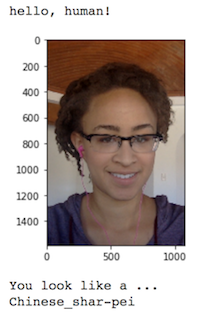
\includegraphics{images/sample_human_output.png}
\caption{Sample Human Output}
\end{figure}

\hypertarget{implementation-write-your-algorithm}{%
\subsubsection{(IMPLEMENTATION) Write your
Algorithm}\label{implementation-write-your-algorithm}}

    \hypertarget{method-1}{%
\subsubsection{method 1}\label{method-1}}

    \begin{Verbatim}[commandchars=\\\{\}]
{\color{incolor}In [{\color{incolor}130}]:} \PY{k}{def} \PY{n+nf}{dog\PYZus{}human\PYZus{}detector}\PY{p}{(}\PY{n}{img\PYZus{}path}\PY{p}{)}\PY{p}{:}
              \PY{c+c1}{\PYZsh{}\PYZsh{}\PYZsh{}}
              \PY{k}{if} \PY{n}{dog\PYZus{}detector\PYZus{}net50}\PY{p}{(}\PY{n}{img\PYZus{}path}\PY{p}{)} \PY{o}{\PYZgt{}} \PY{l+m+mi}{0}\PY{p}{:} 
                  \PY{n}{is\PYZus{}human} \PY{o}{=} \PY{k+kc}{False}
                  \PY{n}{dog\PYZus{}breed} \PY{o}{=} \PY{n}{predict\PYZus{}breed\PYZus{}transfer}\PY{p}{(}\PY{n}{img\PYZus{}path}\PY{p}{)}        
              \PY{c+c1}{\PYZsh{} use Haarscascade model to detect whether a human or not}
              \PY{k}{elif} \PY{n}{face\PYZus{}detector}\PY{p}{(}\PY{n}{img\PYZus{}path}\PY{p}{)} \PY{o}{\PYZgt{}} \PY{l+m+mi}{0}\PY{p}{:} 
                  \PY{n}{is\PYZus{}human} \PY{o}{=} \PY{k+kc}{True} 
                  \PY{n}{dog\PYZus{}breed} \PY{o}{=} \PY{n}{predict\PYZus{}breed\PYZus{}transfer}\PY{p}{(}\PY{n}{img\PYZus{}path}\PY{p}{)}
              \PY{k}{else} \PY{p}{:} 
                   \PY{k}{return} \PY{o}{\PYZhy{}}\PY{l+m+mi}{1}
              \PY{k}{return} \PY{n}{is\PYZus{}human}\PY{p}{,} \PY{n}{dog\PYZus{}breed}
\end{Verbatim}


    \begin{Verbatim}[commandchars=\\\{\}]
{\color{incolor}In [{\color{incolor}131}]:} \PY{c+c1}{\PYZsh{}\PYZsh{}\PYZsh{} TODO: Write your algorithm.}
          \PY{c+c1}{\PYZsh{}\PYZsh{}\PYZsh{} Feel free to use as many code cells as needed.}
          
          \PY{k}{def} \PY{n+nf}{run\PYZus{}app}\PY{p}{(}\PY{n}{img\PYZus{}path}\PY{p}{)}\PY{p}{:}
              \PY{c+c1}{\PYZsh{}\PYZsh{} handle cases for a human face, dog, and neither}
              \PY{n}{is\PYZus{}human}\PY{p}{,} \PY{n}{dog\PYZus{}breed} \PY{o}{=} \PY{n}{dog\PYZus{}human\PYZus{}detector}\PY{p}{(}\PY{n}{img\PYZus{}path}\PY{p}{)}
              \PY{n+nb}{print}\PY{p}{(}\PY{l+s+s2}{\PYZdq{}}\PY{l+s+s2}{the path of the file:}\PY{l+s+s2}{\PYZdq{}}\PY{p}{,} \PY{n}{img\PYZus{}path}\PY{p}{)}
              \PY{c+c1}{\PYZsh{}\PYZsh{} display the image}
              \PY{n}{img} \PY{o}{=} \PY{n}{cv2}\PY{o}{.}\PY{n}{imread}\PY{p}{(}\PY{n}{img\PYZus{}path}\PY{p}{)}
              \PY{n}{cv\PYZus{}rgb} \PY{o}{=} \PY{n}{cv2}\PY{o}{.}\PY{n}{cvtColor}\PY{p}{(}\PY{n}{img}\PY{p}{,} \PY{n}{cv2}\PY{o}{.}\PY{n}{COLOR\PYZus{}BGR2RGB}\PY{p}{)}
              \PY{n}{imgplot} \PY{o}{=} \PY{n}{plt}\PY{o}{.}\PY{n}{imshow}\PY{p}{(}\PY{n}{cv\PYZus{}rgb}\PY{p}{)}
              \PY{n}{plt}\PY{o}{.}\PY{n}{show}\PY{p}{(}\PY{p}{)}    
              \PY{k}{if}\PY{p}{(}\PY{n}{is\PYZus{}human} \PY{o}{==} \PY{k+kc}{True}\PY{p}{)}\PY{p}{:}
                  \PY{n+nb}{print}\PY{p}{(}\PY{l+s+s2}{\PYZdq{}}\PY{l+s+s2}{Hello human, You look like a ... }\PY{l+s+s2}{\PYZdq{}}\PY{p}{,}\PY{n}{dog\PYZus{}breed}\PY{p}{)}
              \PY{k}{else}\PY{p}{:}
                  \PY{n+nb}{print}\PY{p}{(}\PY{l+s+s2}{\PYZdq{}}\PY{l+s+s2}{the breed of dog is:}\PY{l+s+s2}{\PYZdq{}}\PY{p}{,} \PY{n}{dog\PYZus{}breed}\PY{p}{)}
\end{Verbatim}


    \hypertarget{method-2}{%
\subsubsection{method 2}\label{method-2}}

    \begin{Verbatim}[commandchars=\\\{\}]
{\color{incolor}In [{\color{incolor}132}]:} \PY{c+c1}{\PYZsh{}\PYZsh{}\PYZsh{} TODO: Write your algorithm.}
          \PY{c+c1}{\PYZsh{}\PYZsh{}\PYZsh{} Feel free to use as many code cells as needed.}
          \PY{k}{if} \PY{n}{use\PYZus{}cuda}\PY{p}{:}
              \PY{n}{model\PYZus{}transfer}\PY{o}{.}\PY{n}{load\PYZus{}state\PYZus{}dict}\PY{p}{(}\PY{n}{torch}\PY{o}{.}\PY{n}{load}\PY{p}{(}\PY{l+s+s1}{\PYZsq{}}\PY{l+s+s1}{model\PYZus{}transfer.pt}\PY{l+s+s1}{\PYZsq{}}\PY{p}{)}\PY{p}{)}
          \PY{k}{else} \PY{p}{:}
              \PY{n}{model\PYZus{}transfer}\PY{o}{.}\PY{n}{load\PYZus{}state\PYZus{}dict}\PY{p}{(}\PY{n}{torch}\PY{o}{.}\PY{n}{load}\PY{p}{(}\PY{l+s+s1}{\PYZsq{}}\PY{l+s+s1}{model\PYZus{}transfer.pt}\PY{l+s+s1}{\PYZsq{}}\PY{p}{,} \PY{n}{map\PYZus{}location}\PY{o}{=}\PY{l+s+s1}{\PYZsq{}}\PY{l+s+s1}{cpu}\PY{l+s+s1}{\PYZsq{}}\PY{p}{)}\PY{p}{)}
          
          \PY{k}{def} \PY{n+nf}{run\PYZus{}app}\PY{p}{(}\PY{n}{img\PYZus{}path}\PY{p}{)}\PY{p}{:}
              \PY{n}{dog\PYZus{}breed} \PY{o}{=} \PY{n}{predict\PYZus{}breed\PYZus{}transfer}\PY{p}{(}\PY{n}{img\PYZus{}path}\PY{p}{)} 
              
              \PY{n+nb}{print}\PY{p}{(}\PY{l+s+s2}{\PYZdq{}}\PY{l+s+s2}{the path of the file:}\PY{l+s+s2}{\PYZdq{}}\PY{p}{,} \PY{n}{img\PYZus{}path}\PY{p}{)}
              \PY{c+c1}{\PYZsh{}\PYZsh{} Display the image}
              \PY{n}{img} \PY{o}{=} \PY{n}{cv2}\PY{o}{.}\PY{n}{imread}\PY{p}{(}\PY{n}{img\PYZus{}path}\PY{p}{)}
              \PY{n}{cv\PYZus{}rgb} \PY{o}{=} \PY{n}{cv2}\PY{o}{.}\PY{n}{cvtColor}\PY{p}{(}\PY{n}{img}\PY{p}{,} \PY{n}{cv2}\PY{o}{.}\PY{n}{COLOR\PYZus{}BGR2RGB}\PY{p}{)}
              \PY{n}{plt}\PY{o}{.}\PY{n}{imshow}\PY{p}{(}\PY{n}{cv\PYZus{}rgb}\PY{p}{)}
              \PY{n}{plt}\PY{o}{.}\PY{n}{show}\PY{p}{(}\PY{p}{)}
              
              \PY{c+c1}{\PYZsh{}\PYZsh{} handle cases for a human face, dog, and neither}
              \PY{k}{if} \PY{n}{dog\PYZus{}detector\PYZus{}net50}\PY{p}{(}\PY{n}{img\PYZus{}path}\PY{p}{)}\PY{p}{:}
                  \PY{n+nb}{print}\PY{p}{(}\PY{l+s+s2}{\PYZdq{}}\PY{l+s+s2}{Hello! The predicted dog breed is: }\PY{l+s+si}{\PYZob{}\PYZcb{}}\PY{l+s+s2}{\PYZdq{}}\PY{o}{.}\PY{n}{format}\PY{p}{(}\PY{n}{dog\PYZus{}breed}\PY{p}{)}\PY{p}{)}
              \PY{k}{elif} \PY{n}{face\PYZus{}detector}\PY{p}{(}\PY{n}{img\PYZus{}path}\PY{p}{)}\PY{p}{:}
                  \PY{n+nb}{print}\PY{p}{(}\PY{l+s+s2}{\PYZdq{}}\PY{l+s+s2}{Hello human, You look like a ...:}\PY{l+s+si}{\PYZob{}\PYZcb{}}\PY{l+s+s2}{\PYZdq{}}\PY{o}{.}\PY{n}{format}\PY{p}{(}\PY{n}{dog\PYZus{}breed}\PY{p}{)}\PY{p}{)}
              \PY{k}{else}\PY{p}{:}
                  \PY{n+nb}{print}\PY{p}{(}\PY{l+s+s2}{\PYZdq{}}\PY{l+s+s2}{Error, Alien}\PY{l+s+s2}{\PYZdq{}}\PY{p}{)}
                  \PY{c+c1}{\PYZsh{}\PYZsh{} return error message and break function}
\end{Verbatim}


    \begin{center}\rule{0.5\linewidth}{\linethickness}\end{center}

 \#\# Step 6: Test Your Algorithm

In this section, you will take your new algorithm for a spin! What kind
of dog does the algorithm think that \emph{you} look like? If you have a
dog, does it predict your dog's breed accurately? If you have a cat,
does it mistakenly think that your cat is a dog?

\hypertarget{implementation-test-your-algorithm-on-sample-images}{%
\subsubsection{(IMPLEMENTATION) Test Your Algorithm on Sample
Images!}\label{implementation-test-your-algorithm-on-sample-images}}

Test your algorithm at least six images on your computer. Feel free to
use any images you like. Use at least two human and two dog images.

\textbf{Question 6:} Is the output better than you expected :) ? Or
worse :( ? Provide at least three possible points of improvement for
your algorithm.

    \textbf{Answer:} The output is better than I expected, the test accuracy
increased from approximately 21\% to 84\%. The transfer learning with
Resnet-50 together provides a pretty satisfied result when compared to
the original CNN I created in section 3. I am especially surprised by
the predicted label American eskimo dog, my dog summer is in fact a
Samoyed, it is very close. * The improvements can start with data
argumentation, to make the model more generalized to fit different type
of dogs. We can change the data agumentation parameters to test the
accuracy. * The second way is to train the current model on a larger
data sets. * The third, we can modify the hyper-parameters
(e.g.~learning rate) until we have an optimal choices of
hyper-parameters. However, this approach is very time consuming, hundres
of hours of calculation are expected, alternative solution would be
parallel computing. * We can add more dense layers to the pretrained
networks, for example, an additional dense layer before the final linear
layer would slightly increase the accuracy.

    \begin{Verbatim}[commandchars=\\\{\}]
{\color{incolor}In [{\color{incolor}140}]:} \PY{c+c1}{\PYZsh{}\PYZsh{} TODO: Execute your algorithm from Step 6 on}
          \PY{c+c1}{\PYZsh{}\PYZsh{} at least 6 images on your computer.}
          \PY{c+c1}{\PYZsh{}\PYZsh{} Feel free to use as many code cells as needed.}
          
          \PY{c+c1}{\PYZsh{}\PYZsh{} in online notebook I use existing files instead of my own images}
          \PY{c+c1}{\PYZsh{}\PYZsh{} suggested code, below}
          \PY{n}{human\PYZus{}files\PYZus{}user} \PY{o}{=} \PY{n}{np}\PY{o}{.}\PY{n}{array}\PY{p}{(}\PY{n}{glob}\PY{p}{(}\PY{l+s+s2}{\PYZdq{}}\PY{l+s+s2}{lfw\PYZus{}user/*}\PY{l+s+s2}{\PYZdq{}}\PY{p}{)}\PY{p}{)}
          \PY{n}{dog\PYZus{}files\PYZus{}user} \PY{o}{=} \PY{n}{np}\PY{o}{.}\PY{n}{array}\PY{p}{(}\PY{n}{glob}\PY{p}{(}\PY{l+s+s2}{\PYZdq{}}\PY{l+s+s2}{dogImages\PYZus{}user/*}\PY{l+s+s2}{\PYZdq{}}\PY{p}{)}\PY{p}{)}
          
          \PY{k}{for} \PY{n}{file} \PY{o+ow}{in} \PY{n}{np}\PY{o}{.}\PY{n}{hstack}\PY{p}{(}\PY{p}{(}\PY{n}{human\PYZus{}files\PYZus{}user}\PY{p}{[}\PY{p}{:}\PY{l+m+mi}{6}\PY{p}{]}\PY{p}{,} \PY{n}{dog\PYZus{}files\PYZus{}user}\PY{p}{[}\PY{p}{:}\PY{l+m+mi}{9}\PY{p}{]}\PY{p}{)}\PY{p}{)}\PY{p}{:}
          \PY{c+c1}{\PYZsh{}for file in np.hstack((human\PYZus{}files[:3], dog\PYZus{}files[:3])):}
              \PY{n}{run\PYZus{}app}\PY{p}{(}\PY{n}{file}\PY{p}{)}
\end{Verbatim}


    \begin{Verbatim}[commandchars=\\\{\}]
torch.Size([1, 3, 224, 224])
the path of the file: lfw\_user/Abdel\_Aziz\_Al-Hakim\_0001.jpg

    \end{Verbatim}

    \begin{center}
    \adjustimage{max size={0.9\linewidth}{0.9\paperheight}}{output_75_1.png}
    \end{center}
    { \hspace*{\fill} \\}
    
    \begin{Verbatim}[commandchars=\\\{\}]
Hello human, You look like a {\ldots}:Portuguese water dog
torch.Size([1, 3, 224, 224])
the path of the file: lfw\_user/IMG\_1353.png

    \end{Verbatim}

    \begin{center}
    \adjustimage{max size={0.9\linewidth}{0.9\paperheight}}{output_75_3.png}
    \end{center}
    { \hspace*{\fill} \\}
    
    \begin{Verbatim}[commandchars=\\\{\}]
Error, Alien
torch.Size([1, 3, 224, 224])
the path of the file: lfw\_user/star.png

    \end{Verbatim}

    \begin{center}
    \adjustimage{max size={0.9\linewidth}{0.9\paperheight}}{output_75_5.png}
    \end{center}
    { \hspace*{\fill} \\}
    
    \begin{Verbatim}[commandchars=\\\{\}]
Hello human, You look like a {\ldots}:Chinese crested
torch.Size([1, 3, 224, 224])
the path of the file: lfw\_user/Vladimir.png

    \end{Verbatim}

    \begin{center}
    \adjustimage{max size={0.9\linewidth}{0.9\paperheight}}{output_75_7.png}
    \end{center}
    { \hspace*{\fill} \\}
    
    \begin{Verbatim}[commandchars=\\\{\}]
Hello human, You look like a {\ldots}:Parson russell terrier
torch.Size([1, 3, 224, 224])
the path of the file: lfw\_user/thomas.JPG

    \end{Verbatim}

    \begin{center}
    \adjustimage{max size={0.9\linewidth}{0.9\paperheight}}{output_75_9.png}
    \end{center}
    { \hspace*{\fill} \\}
    
    \begin{Verbatim}[commandchars=\\\{\}]
Hello human, You look like a {\ldots}:Plott
torch.Size([1, 3, 224, 224])
the path of the file: lfw\_user/rapper.png

    \end{Verbatim}

    \begin{center}
    \adjustimage{max size={0.9\linewidth}{0.9\paperheight}}{output_75_11.png}
    \end{center}
    { \hspace*{\fill} \\}
    
    \begin{Verbatim}[commandchars=\\\{\}]
Hello human, You look like a {\ldots}:Xoloitzcuintli
torch.Size([1, 3, 224, 224])
the path of the file: dogImages\_user/Lhasa\_apso\_06649.jpg

    \end{Verbatim}

    \begin{center}
    \adjustimage{max size={0.9\linewidth}{0.9\paperheight}}{output_75_13.png}
    \end{center}
    { \hspace*{\fill} \\}
    
    \begin{Verbatim}[commandchars=\\\{\}]
Hello! The predicted dog breed is: Havanese
torch.Size([1, 3, 224, 224])
the path of the file: dogImages\_user/IMG\_1627.jpg

    \end{Verbatim}

    \begin{center}
    \adjustimage{max size={0.9\linewidth}{0.9\paperheight}}{output_75_15.png}
    \end{center}
    { \hspace*{\fill} \\}
    
    \begin{Verbatim}[commandchars=\\\{\}]
Hello! The predicted dog breed is: American eskimo dog
torch.Size([1, 3, 224, 224])
the path of the file: dogImages\_user/Yorkshire\_terrier\_08348.jpg

    \end{Verbatim}

    \begin{center}
    \adjustimage{max size={0.9\linewidth}{0.9\paperheight}}{output_75_17.png}
    \end{center}
    { \hspace*{\fill} \\}
    
    \begin{Verbatim}[commandchars=\\\{\}]
Hello! The predicted dog breed is: Yorkshire terrier
torch.Size([1, 3, 224, 224])
the path of the file: dogImages\_user/german shepherd\_4.jpg

    \end{Verbatim}

    \begin{center}
    \adjustimage{max size={0.9\linewidth}{0.9\paperheight}}{output_75_19.png}
    \end{center}
    { \hspace*{\fill} \\}
    
    \begin{Verbatim}[commandchars=\\\{\}]
Hello! The predicted dog breed is: Keeshond
torch.Size([1, 3, 224, 224])
the path of the file: dogImages\_user/Black\_russian\_terrier\_01837.jpg

    \end{Verbatim}

    \begin{center}
    \adjustimage{max size={0.9\linewidth}{0.9\paperheight}}{output_75_21.png}
    \end{center}
    { \hspace*{\fill} \\}
    
    \begin{Verbatim}[commandchars=\\\{\}]
Hello! The predicted dog breed is: Black russian terrier
torch.Size([1, 3, 224, 224])
the path of the file: dogImages\_user/german shepherd\_5.jpg

    \end{Verbatim}

    \begin{center}
    \adjustimage{max size={0.9\linewidth}{0.9\paperheight}}{output_75_23.png}
    \end{center}
    { \hspace*{\fill} \\}
    
    \begin{Verbatim}[commandchars=\\\{\}]
Hello! The predicted dog breed is: Akita
torch.Size([1, 3, 224, 224])
the path of the file: dogImages\_user/german shepherd\_1.jpg

    \end{Verbatim}

    \begin{center}
    \adjustimage{max size={0.9\linewidth}{0.9\paperheight}}{output_75_25.png}
    \end{center}
    { \hspace*{\fill} \\}
    
    \begin{Verbatim}[commandchars=\\\{\}]
Hello! The predicted dog breed is: Alaskan malamute
torch.Size([1, 3, 224, 224])
the path of the file: dogImages\_user/german shepherd\_2.JPG

    \end{Verbatim}

    \begin{center}
    \adjustimage{max size={0.9\linewidth}{0.9\paperheight}}{output_75_27.png}
    \end{center}
    { \hspace*{\fill} \\}
    
    \begin{Verbatim}[commandchars=\\\{\}]
Hello! The predicted dog breed is: Icelandic sheepdog
torch.Size([1, 3, 224, 224])
the path of the file: dogImages\_user/german shepherd\_3.jpg

    \end{Verbatim}

    \begin{center}
    \adjustimage{max size={0.9\linewidth}{0.9\paperheight}}{output_75_29.png}
    \end{center}
    { \hspace*{\fill} \\}
    
    \begin{Verbatim}[commandchars=\\\{\}]
Hello! The predicted dog breed is: Keeshond

    \end{Verbatim}


    % Add a bibliography block to the postdoc
    
    
    
    \end{document}
